\documentclass{article}

  % packages
    % basic stuff for rendering math
    \usepackage[letterpaper, top=1in, bottom=1in, left=1in, right=1in]{geometry}
    \usepackage[utf8]{inputenc}
    \usepackage[english]{babel}
    \usepackage{amsmath} 
    \usepackage{amssymb}
    \usepackage{bookmark}

    % extra math symbols and utilities
    \usepackage{mathtools}        % for extra stuff like \coloneqq
    \usepackage{mathrsfs}         % for extra stuff like \mathsrc{}
    \usepackage{centernot}        % for the centernot arrow 
    \usepackage{bm}               % for better boldsymbol/mathbf 
    \usepackage{enumitem}         % better control over enumerate, itemize
    \usepackage{hyperref}         % for hypertext linking
    \usepackage{xr-hyper}
    \usepackage{fancyvrb}          % for better verbatim environments
    \usepackage{newverbs}         % for texttt{}
    \usepackage{xcolor}           % for colored text 
    \usepackage{listings}         % to include code
    \usepackage{lstautogobble}    % helper package for code
    \usepackage{parcolumns}       % for side by side columns for two column code
    \usepackage{algorithm}
    \usepackage{algpseudocode}
    \usepackage{bbm}
    \algblock{Class}{EndClass}

    % page layout
    \usepackage{fancyhdr}         % for headers and footers 
    \usepackage{uniquecounter}
    \usepackage{lastpage}         % to include last page number in footer 
    \usepackage{parskip}          % for no indentation and space between paragraphs   
    \usepackage[T1]{fontenc}      % to include \textbackslash
    \usepackage{footnote}
    \usepackage{etoolbox}

    % for custom environments
    \usepackage{tcolorbox}        % for better colored boxes in custom environments
    \tcbuselibrary{breakable}     % to allow tcolorboxes to break across pages

    % figures
    \usepackage{pgfplots}
    \pgfplotsset{compat=1.18}
    \usepackage{float}            % for [H] figure placement
    \usepackage{tikz}
    \usepackage{tikz-cd}
    \usepackage{circuitikz}
    \usetikzlibrary{arrows, arrows.meta}
    \usetikzlibrary{positioning}
    \usetikzlibrary{calc}
    \usepackage{graphicx}
    \usepackage{caption} 
    \usepackage{subcaption}
    \captionsetup{font=small} 

    % for tabular stuff 
    \usepackage{dcolumn}

    \usepackage[nottoc]{tocbibind}
    \pdfsuppresswarningpagegroup=1
    \hfuzz=5.002pt                % ignore overfull hbox badness warnings below this limit

  % New and replaced operators
    \DeclareMathOperator{\Tr}{Tr}
    \DeclareMathOperator{\Sym}{Sym}
    \DeclareMathOperator{\Span}{span}
    \DeclareMathOperator{\elbo}{ELBO}
    \DeclareMathOperator{\std}{std}
    \DeclareMathOperator{\Cov}{Cov}
    \DeclareMathOperator{\Var}{Var}
    \DeclareMathOperator{\Corr}{Corr}
    \DeclareMathOperator{\pos}{pos}
    \DeclareMathOperator*{\argmin}{\arg\!\min}
    \DeclareMathOperator*{\argmax}{\arg\!\max}
    \newcommand{\qed}{\hfill$\blacksquare$}     % I like QED squares to be black

  % Custom Environments
    \newtcolorbox[auto counter, number within=section]{question}[1][]
    {
      colframe = orange!25,
      colback  = orange!10,
      coltitle = orange!20!black,  
      breakable, 
      title = \textbf{Question \thetcbcounter ~(#1)}
    }

    \newtcolorbox[auto counter, number within=section]{exercise}[1][]
    {
      colframe = teal!25,
      colback  = teal!10,
      coltitle = teal!20!black,  
      breakable, 
      title = \textbf{Exercise \thetcbcounter ~(#1)}
    }
    \newtcolorbox[auto counter, number within=section]{solution}[1][]
    {
      colframe = violet!25,
      colback  = violet!10,
      coltitle = violet!20!black,  
      breakable, 
      title = \textbf{Solution \thetcbcounter}
    }
    \newtcolorbox[auto counter, number within=section]{lemma}[1][]
    {
      colframe = red!25,
      colback  = red!10,
      coltitle = red!20!black,  
      breakable, 
      title = \textbf{Lemma \thetcbcounter ~(#1)}
    }
    \newtcolorbox[auto counter, number within=section]{theorem}[1][]
    {
      colframe = red!25,
      colback  = red!10,
      coltitle = red!20!black,  
      breakable, 
      title = \textbf{Theorem \thetcbcounter ~(#1)}
    } 
    \newtcolorbox[auto counter, number within=section]{corollary}[1][]
    {
      colframe = red!25,
      colback  = red!10,
      coltitle = red!20!black,  
      breakable, 
      title = \textbf{Corollary \thetcbcounter ~(#1)}
    } 
    \newtcolorbox[auto counter, number within=section]{proof}[1][]
    {
      colframe = orange!25,
      colback  = orange!10,
      coltitle = orange!20!black,  
      breakable, 
      title = \textbf{Proof. }
    } 
    \newtcolorbox[auto counter, number within=section]{definition}[1][]
    {
      colframe = yellow!25,
      colback  = yellow!10,
      coltitle = yellow!20!black,  
      breakable, 
      title = \textbf{Definition \thetcbcounter ~(#1)}
    } 
    \newtcolorbox[auto counter, number within=section]{example}[1][]
    {
      colframe = blue!25,
      colback  = blue!10,
      coltitle = blue!20!black,  
      breakable, 
      title = \textbf{Example \thetcbcounter ~(#1)}
    } 
    \newtcolorbox[auto counter, number within=section]{code}[1][]
    {
      colframe = green!25,
      colback  = green!10,
      coltitle = green!20!black,  
      breakable, 
      title = \textbf{Code \thetcbcounter ~(#1)}
    } 
    \newtcolorbox[auto counter, number within=section]{algo}[1][]
    {
      colframe = green!25,
      colback  = green!10,
      coltitle = green!20!black,  
      breakable, 
      title = \textbf{Algorithm \thetcbcounter ~(#1)}
    } 
    \definecolor{cverbbg}{gray}{0.93}
    \newenvironment{cverbatim}
      {\SaveVerbatim{cverb}}
      {\endSaveVerbatim
        \flushleft\fboxrule=0pt\fboxsep=.5em
        \colorbox{cverbbg}{%
          \makebox[\dimexpr\linewidth-2\fboxsep][l]{\BUseVerbatim{cverb}}%
        }
        \endflushleft
    }

    \definecolor{dkgreen}{rgb}{0,0.6,0}
    \definecolor{gray}{rgb}{0.5,0.5,0.5}
    \definecolor{mauve}{rgb}{0.58,0,0.82}
    \definecolor{lightgray}{gray}{0.93}
    \renewcommand{\algorithmiccomment}[1]{\hfill$\triangleright$\textcolor{blue}{#1}}

    % default options for listings (for code)
    \lstset{
      autogobble,
      frame=ltbr,
      language=Python,                           % the language of the code
      aboveskip=3mm,
      belowskip=3mm,
      showstringspaces=false,
      columns=fullflexible,
      keepspaces=true,
      basicstyle={\small\ttfamily},
      numbers=left,
      firstnumber=1,                        % start line number at 1
      numberstyle=\tiny\color{gray},
      keywordstyle=\color{blue},
      commentstyle=\color{dkgreen},
      stringstyle=\color{mauve},
      backgroundcolor=\color{lightgray}, 
      breaklines=true,                      % break lines
      breakatwhitespace=true,
      tabsize=3, 
      xleftmargin=2em, 
      framexleftmargin=1.5em, 
      stepnumber=1
    }

  % Page style
    \pagestyle{fancy}
    \fancyhead[L]{}
    \fancyhead[C]{Muchang Bahng}
    \fancyhead[R]{Spring 2023} 
    \fancyfoot[C]{\thepage / \pageref{LastPage}}
    \renewcommand{\footrulewidth}{0.4pt}          % the footer line should be 0.4pt wide
    \renewcommand{\thispagestyle}[1]{}  % needed to include headers in title page
%    \renewcommand{\thefootnote}{\arabic{footnote}}

  % external documents 
    \externaldocument[algo-]{../../Computer_Science/DSA/paper}[../../Computer_Science/DSA/paper.pdf]

\begin{document}

\tikzset{every picture/.style={line width=0.75pt}} 

\title{}
\author{Muchang Bahng}
\date{Spring 2023}

\maketitle
\tableofcontents
\pagebreak 


This covers computability theory, complexity theory, and automata theory. 
Alphabet. Boolean logic


\section{Multi-Layered Perceptrons} 

  We build upon what we already know: generalized linear models. In simple regression, we transform the inputs into the relevant features $\mathbf{x}_n \mapsto \boldsymbol{\phi} (\mathbf{x}_n) = \boldsymbol{\phi}_n$ and then, when we construct a generalized linear model, we assume that the conditional distribution $Y \mid X = x$ is in the canonical exponential family, with some natural parameter $\eta(x)$ and expected mean $\mu(x) = \mathbb{E}[Y \mid X = x]$. Then, to choose the link function $g$ that related $g(\mu(x)) = x^T \beta$, we can set it to be the canonical link $g$ that maps $\mu$ to $\eta$. That is, we have $g(\mu(x)) = x^T \beta = \eta (x)$ such that the natural parameter is linearly dependent on the input. The inverse $g^{-1}$ of the link function is called the \textbf{activation function}, which connects the expected mean to a linear function of $x$. 
  \begin{equation}
    h_\beta (x) = g^{-1} (x^T \beta) = \mu(x) = \mathbb{E}[Y \mid X = x]
  \end{equation}
  Now, note that for a classification problem, the decision boundary defined in the $\boldsymbol{\phi}$ feature space is linear, but it may not be linear in the input space $\mathcal{X}$. We would like to extend this model by making the basis functions $\boldsymbol{\phi}_n$ depend on the parameters $\mathbf{w}$ and then allow these parameters to be adjusted during training. 

  \begin{figure}[H]
    \centering
    \begin{subfigure}[t]{0.24\textwidth}
      \centering
      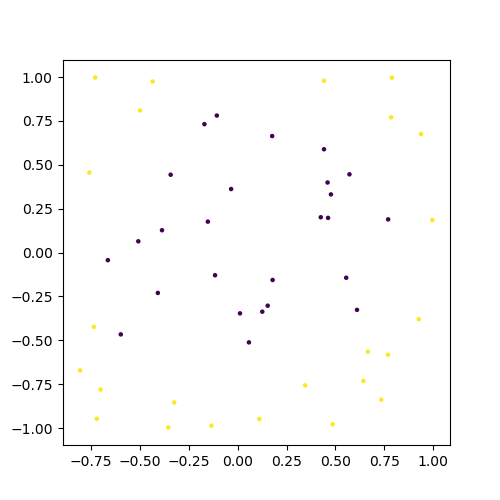
\includegraphics[width=\textwidth]{img/untrans_data.png}
      \caption{Data in space $\mathcal{X} = \mathbb{R}^2$.}
      \label{fig:raw_points}
    \end{subfigure}
    \hfill
    \begin{subfigure}[t]{0.24\textwidth}
      \centering
      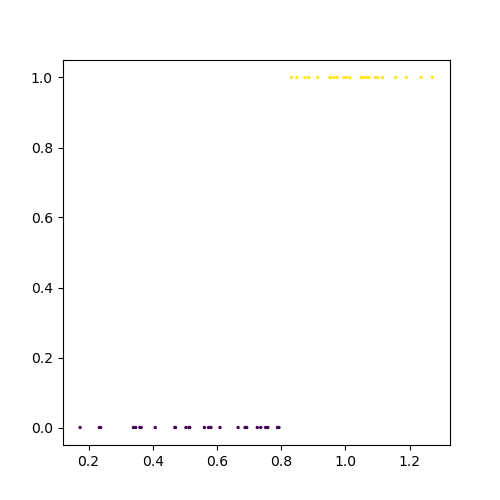
\includegraphics[width=\textwidth]{img/trans_data.png}
      \caption{Transformed data $\phi(\mathbf{x}) = \|\mathbf{x}\|$.}
      \label{fig:transformed_points}
    \end{subfigure}
    \hfill
    \begin{subfigure}[t]{0.24\textwidth}
      \centering
      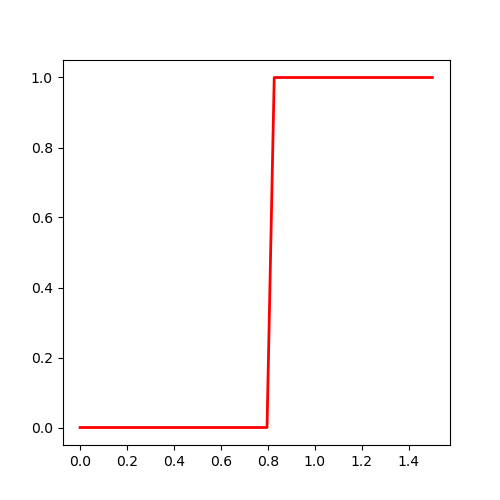
\includegraphics[width=\textwidth]{img/trans_fit.png}
      \caption{Logistic fit in transformed space.}
      \label{fig:transformed_trained}
    \end{subfigure}
    \hfill
    \begin{subfigure}[t]{0.24\textwidth}
      \centering
      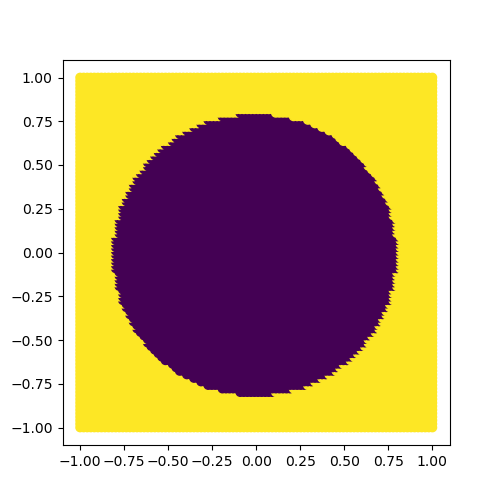
\includegraphics[width=\textwidth]{img/untrans_fit.png}
      \caption{Logistic fit to data in input space.}
      \label{fig:raw_trained}
    \end{subfigure}
    \caption{Consider the set of points in $\mathbb{R}^2$ with the corresponding class. We transform the features to $\boldsymbol{\phi}(x_1, x_2) = x_1^2 + x_2^2$, which gives us a new space to work with. Fitting logistic regression onto this gives a linear decision boundary in the space $\boldsymbol{\phi}$, but the boundary is circular in $\mathcal{X} = \mathbb{R}^2$.}
    \label{fig:logistic_transformed}
  \end{figure}

\subsection{Feedforward Fully-Connected Networks}

  So how should we construct parametric nonlinear basis functions? One way is to have a similar architecture as GLMs by having a linear map followed by an activation function $f(x) = \sigma(w^T x + b)$. The simplest such function with the activation function as the step function 
  \begin{equation}
    f(z) = \begin{cases} 1 & \text{ if } z \geq 0 \\ 0 & \text{ if } z < 0 \end{cases}
  \end{equation}
  is the perceptron algorithm. It divides $\mathbb{R}^d$ using a hyperplane $\boldsymbol{\omega}^T \mathbf{x} + b = 0$ and linearly classifies all points on one side to value $1$ and the other side to value $0$. This is similar to a neuron, which takes in a value and outputs a ``signal" if the function evaluated gets past a threshold. However, for reasons regarding training these networks, we would like to use smooth activation functions for this, so we would use different activations. Hence we have a neuron. 

  \begin{definition}[Neuron]
    A \textbf{neuron} is a function of form 
    \begin{equation}
      y = \sigma(\mathbf{w}^T x  + b)
    \end{equation}
    where $\sigma: \mathbb{R} \rightarrow \mathbb{R}$ is any nonlinear function, called an \textbf{activation functions}. 
  \end{definition}
  
  Ultimately, a neural net is really just a generalized linear model with some trained feature extractors, which is why in practice, if researchers want to predict a smaller dataset, they take a pretrained model on a related larger dataset and simply tune the final layer, since the second last layer most likely encodes all the relevant features. This is called \textit{transfer learning}. But historically, it was called a \textit{multilayer perceptron} and the name stuck. 

  \begin{definition}[Feedforward, Fully-Connected Multilayer Perceptron]
    A $L$-layer \textbf{multilayer perceptron (MLP)} $f_\theta : \mathbb{R}^D \rightarrow \mathbb{R}^M$, with parameters $\theta$, is a function of form 
    \begin{equation}
      h_\theta (\mathbf{x}) \coloneqq \sigma^{[L]} \circ W^{[L]} \circ \sigma^{[L-1]} \circ W^{[L-1]} \circ \cdots \circ \sigma^{[1]} \circ W^{[1]} (\mathbf{x})
    \end{equation}
    where $\sigma^{[l]}: \mathbb{R}^{N^{[l]}} \rightarrow \mathbb{R}^{N^{[l]}}$ is an activation function and $W^{[l]}: \mathbb{R}^{N^{[l-1]}} \rightarrow \mathbb{R}^{N^{[l]}}$ is an affine map. We will use the following notation. 
    \begin{enumerate}
      \item The inputs will be labeled $\mathbf{x} = a^{[0]}$ which is in $\mathbb{R}^{N^{[0]}} = \mathbb{R}^D$. 
      
      \item We map $a^{[l]} \in \mathbb{R}^{N^{[l]}} \mapsto W^{[l+1]} a^{[l]} + b^{[l+1]}= z^{[l+1]} \in \mathbb{R}^{N^{[l+1]}}$, where $z$ denotes a vector after an affine transformation. 

      \item We map $z^{[l+1]} \in \mathbb{R}^{N^{[l+1]}} \mapsto \sigma(z^{[l+1]}) = a^{[l+1]} \in \mathbb{R}^{N^{[l+1]}}$, where $a$ denotes a vector after an activation function. 

      \item We keep doing this until we reach the second last layer with vector $a^{[L-1]}$. Note that in the last layer we do \textit{not} apply an activation function. 
    \end{enumerate}

    \begin{figure}[H]
      \centering 
      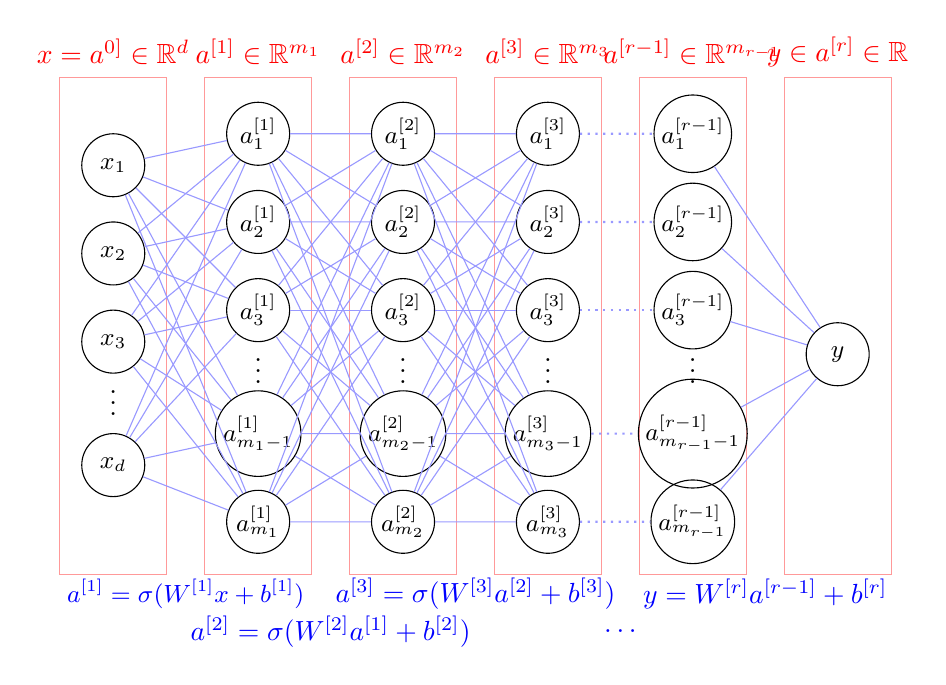
\begin{tikzpicture}[
        scale=0.8, 
        node distance=2cm,
        neuron/.style={circle, draw, minimum size=0.8cm, inner sep=1pt, font=\small},
        annotation/.style={text width=3cm},
        >=latex
      ]
        % Define some variables for consistent spacing
        \def\layersep{2.3}
        \def\neuronsep{1.4}
        \def\boxwidth{1.7}
        \def\boxheight{8}
        
        % Add dimension annotations above boxes in red
        \node[red] at (0, \boxheight/2 + 0.8) {$x = a^{0]} \in \mathbb{R}^d$};
        \node[red] at (\layersep, \boxheight/2 + 0.8) {$a^{[1]} \in \mathbb{R}^{m_1}$};
        \node[red] at (2*\layersep, \boxheight/2 + 0.8) {$a^{[2]} \in \mathbb{R}^{m_2}$};
        \node[red] at (3*\layersep, \boxheight/2 + 0.8) {$a^{[3]} \in \mathbb{R}^{m_3}$};
        \node[red] at (4*\layersep, \boxheight/2 + 0.8) {$a^{[r-1]} \in \mathbb{R}^{m_{r-1}}$};
        \node[red] at (5*\layersep, \boxheight/2 + 0.8) {$y \in a^{[r]} \in \mathbb{R}$};
        
        % Draw boxes
        \foreach \x in {0,1,2,3,4,5} {
            \draw[red!40] (\x*\layersep-\boxwidth/2, -\boxheight/2 + 0.5) rectangle (\x*\layersep+\boxwidth/2, \boxheight/2 + 0.4);
        }
        
        % Input layer (x) with adjusted vertical spacing
        \node[neuron] (x1) at (0, 3) {$x_1$};
        \node[neuron] (x2) at (0, {3-\neuronsep}) {$x_2$};
        \node[neuron] (x3) at (0, {3-2*\neuronsep}) {$x_3$};
        \node at (0, {3-2.6*\neuronsep}) {$\vdots$};
        \node[neuron] (xd) at (0, {3-3.4*\neuronsep}) {$x_d$};
        
        % Hidden layers with matching spacing pattern
        \foreach \l in {1,2,3} {
            \node[neuron] (a\l1) at (\l*\layersep, 3.5) {$a^{[\l]}_1$};
            \node[neuron] (a\l2) at (\l*\layersep, {3.5-\neuronsep}) {$a^{[\l]}_2$};
            \node[neuron] (a\l3) at (\l*\layersep, {3.5-2*\neuronsep}) {$a^{[\l]}_3$};
            \node at (\l*\layersep, {3.5-2.6*\neuronsep}) {$\vdots$};
            \node[neuron] (a\l m1) at (\l*\layersep, {3.5-3.4*\neuronsep}) {$a^{[\l]}_{m_{\l}-1}$};
            \node[neuron] (a\l m) at (\l*\layersep, {3.5-4.4*\neuronsep}) {$a^{[\l]}_{m_{\l}}$};
        }
        
        % Second-to-last layer (r-1)
        \node[neuron] (ar1) at (4*\layersep, 3.5) {$a^{[r-1]}_1$};
        \node[neuron] (ar2) at (4*\layersep, {3.5-\neuronsep}) {$a^{[r-1]}_2$};
        \node[neuron] (ar3) at (4*\layersep, {3.5-2*\neuronsep}) {$a^{[r-1]}_3$};
        \node at (4*\layersep, {3.5-2.6*\neuronsep}) {$\vdots$};
        \node[neuron] (arm1) at (4*\layersep, {3.5-3.4*\neuronsep}) {$a^{[r-1]}_{m_{r-1}-1}$};
        \node[neuron] (arm) at (4*\layersep, {3.5-4.4*\neuronsep}) {$a^{[r-1]}_{m_{r-1}}$};
        
        % Output layer
        \node[neuron] (y) at (5*\layersep, 0) {$y$};
        
        % Add σ annotations below connections
        \node[blue] at (0.5*\layersep, -3.8) {\small $a^{[1]} = \sigma(W^{[1]} x + b^{[1]})$};
        \node[blue] at (1.5*\layersep, -4.4) {$a^{[2]} = \sigma(W^{[2]} a^{[1]} + b^{[2]})$};
        \node[blue] at (2.5*\layersep, -3.8) {$a^{[3]} = \sigma(W^{[3]} a^{[2]} + b^{[3]})$};
        \node[blue] at (3.5*\layersep, -4.4) {$\ldots$};
        \node[blue] at (4.5*\layersep, -3.8) {$y = W^{[r]} a^{[r-1]} + b^{[r]}$};
        
        % Draw connections with thinner lines
        \begin{scope}[blue!40, thin]
            % From input to first hidden layer
            \foreach \i in {1,2,3,d} {
                \foreach \j in {1,2,3} {
                    \draw (x\i) -- (a1\j);
                }
                \draw (x\i) -- (a1m1);
                \draw (x\i) -- (a1m);
            }
            
            % Between visible hidden layers
            \foreach \l [remember=\l as \lastl (initially 1)] in {2,3} {
                \foreach \i in {1,2,3} {
                    \foreach \j in {1,2,3} {
                        \draw (a\lastl\i) -- (a\l\j);
                    }
                    \draw (a\lastl\i) -- (a\l m1);
                    \draw (a\lastl\i) -- (a\l m);
                }
                \draw (a\lastl m1) -- (a\l m);
                \draw (a\lastl m1) -- (a\l m1);
                \foreach \j in {1,2,3} {
                    \draw (a\lastl m1) -- (a\l\j);
                }
                \draw (a\lastl m) -- (a\l m);
                \draw (a\lastl m) -- (a\l m1);
                \foreach \j in {1,2,3} {
                    \draw (a\lastl m) -- (a\l\j);
                }
            }
            
            % Dotted connections between layer 3 and r-1
            \foreach \i/\j in {1/1,2/2,3/3} {
                \draw[dotted, thick] (a3\i) -- (ar\j);
            }
            \draw[dotted, thick] (a3m1) -- (arm1);
            \draw[dotted, thick] (a3m) -- (arm);
            
            % From second-to-last to output
            \foreach \i in {1,2,3} {
                \draw (ar\i) -- (y);
            }
            \draw (arm1) -- (y);
            \draw (arm) -- (y);
        \end{scope}
      \end{tikzpicture}
      \caption{If there does not exist any edge from a potential input $x$ to an output $y$, then this means that $x$ is not relevant in calculating $y$, i.e. the weight is $0$. However, we usually work with \textbf{fully-connected neural networks}, which means that every input is relevant to calculating every output, since we usually cannot make assumptions about which variables are relevant or not. }
      \label{fig:multilayer_neural_net}
    \end{figure}
  \end{definition}

  Note that each layer corresponds to how close a neuron is to the output. But really any neuron can be a function of any other neuron. For example, we can connect a neuron from layer $4$ back to a neuron of layer $1$. For now, we will consider networks that are restricted to a \textbf{feed-forward} architecture, in other words having no closed directed cycles. 

  \begin{code}[Parameters and Neural Nets in PyTorch] 
    At this point, you have learned the theory of MLPs. To actually implement them in PyTorch, look at this module \href{code/parameters.ipynb}{here}, which will tell you on how to construct linear maps and activations functions, and more importantly see how you can look at the weights, modify them, and see how they are initialized. You can then learn how to explore the weights and biases of a neural network. 
  \end{code}

\subsection{Forward and Back Propagation}

  Back in the supervised learning notes, we have gone through the derivation for linear, logistic, and softmax regression. It turns out that despite them having very different architectures, with a identity, sigmoid, and softmax activation function, our choice of loss to be the mean squared loss, the binary cross-entropy, and the cross-entropy loss, had given very cute formulas in computing the gradient of the loss. Unfortunately, the formulas do not get cute when we differentiate neural networks, but they do come in a very structured way. To gain intuition, I would recommend to go over the exercises at the end of the chapter labeled ECE 689 Fall 2021 Midterm. If you just use chain rule to do the calculations, you can see that they require us to compute all the intermediate $z^{(i)}$'s and the $a^{(i)}$'s, a process called \textit{forward propagation}, before we compute the gradients. 

  \begin{definition}[Forward Propagation]
    Given an MLP $f$ and an input $x$, the process of sequentially evaluating 
    \begin{equation}
      x = a^{[0]} \mapsto z^{[1]} \mapsto a^{[1]} \mapsto \ldots \mapsto z^{[L]} \mapsto a^{[L]} = f(x)
    \end{equation}
    is called \textbf{forward propagation}. 
  \end{definition} 

  When we want to compute the derivative of $f$. we can see that the intermediate partial derivatives in the chain rule are repeatedly used. That is, if we have layer $0 \leq l \leq L$, then to compute the derivative with respect to the $l$th layer we use the chain rule 
  \begin{equation}
    \frac{\partial f}{\partial z^{[l]}} = \frac{\partial f}{\partial z^{[l+1]}} \cdot \frac{z^{[l+1]}}{z^{[l]}}
  \end{equation}
  which requires us to know the derivative at the $(l+1)$th layer, along with the current values of $z^{[l]}, z^{[l+1]}$ to evaluate the derivatives at the current point. Therefore, we must complete forward propagation first and then compute \textit{backwards} from the result to the input to compute the gradients. 

  \begin{definition}[Backward Propagation]
    Given an MLP $f$ with input $x$ that has been forward propagated, the process of sequentially evaluating 
    \begin{equation}
      \frac{\partial f}{\partial a^{[L]}} \mapsto \frac{\partial f}{\partial z^{[L]}} \mapsto \ldots \mapsto \frac{\partial f}{\partial z^{[L]}}, 
    \end{equation}
    is called \textbf{backward propagation}, or \textbf{backprop}. 
  \end{definition}

  Backpropagation is not hard, but it is cumbersome notation-wise. What we really want to do is just compute a very long vector with all of its partials $\partial E / \partial \boldsymbol{\theta}$. 

  \begin{algo}[Backpropagation]
    To compute $\frac{\partial E_n}{\partial w_{ji}^{[l]}}$, it would be natural to split it up into a portion where $E_n$ is affected by the term before activation $\mathbf{z}^{[l]}$ and how that is affected by $w_{ji}^{[l]}$. The same goes for the bias terms. 
    \begin{equation}
      \frac{\partial E_n}{\partial w_{ji}^{[l]}} = \underbrace{\frac{\partial E_n}{\partial \mathbf{z}^{[l]}}}_{1 \times N^{[l]}} \cdot \underbrace{\frac{\partial \mathbf{z}^{[l]}}{\partial w_{ji}^{[l]}}}_{N^{[l]} \times 1} \text{ and } \frac{\partial E_n}{\partial b_{i}^{[l]}} = \underbrace{\frac{\partial E_n}{\partial \mathbf{z}^{[l]}}}_{1 \times N^{[l]}} \cdot \underbrace{\frac{\partial \mathbf{z}^{[l]}}{\partial b_{i}^{[l]}}}_{N^{[l]} \times 1}
    \end{equation}
    It helps to visualize that we are focusing on 
    \begin{equation}
      \mathbf{h}_{\boldsymbol{\theta}} (\mathbf{x}) = g\big( \ldots \sigma( \underbrace{\mathbf{W}^{[l]} \mathbf{a}^{[l-1]} + \mathbf{b}^{[l]}}_{\mathbf{z}^{[l]}} )  \ldots \big)
    \end{equation}
    We can expand $\mathbf{z}^{[l]}$ to get 
    \begin{equation}
      \mathbf{z}^{[l]} = \begin{pmatrix} w_{11}^{[l]} & \ldots & w_{1 N^{[l-1]}}^{[l]} \\ \vdots & \ddots & \vdots \\ w_{N^{[l]} 1}^{[l]} & \ldots & w_{N^{[l]} N^{[l-1]}}^{[l]} \end{pmatrix} 
      \begin{pmatrix} a^{[l-1]}_1 \\ \vdots \\ a^{[l-1]}_{N^{[l-1]}} \end{pmatrix} + \begin{pmatrix} b_1^{[l]} \\ \vdots \\ b_{N^{[l]}_{[l]}} \end{pmatrix}
    \end{equation}
    $w_{ji}^{[l]}$ will only show up in the $j$th term of $\mathbf{z}^{[l]}$, and so the rest of the terms in $\frac{\partial \mathbf{z}^{[l]}}{\partial w_{ji}^{[l]}}$ will vanish. The same logic applies to $\frac{\partial \mathbf{z}^{[l]}}{\partial b_{i}^{[l]}}$, and so we really just have to compute 
    \begin{equation}
      \frac{\partial E_n}{\partial w_{ji}^{[l]}} = \underbrace{\frac{\partial E_n}{\partial z^{[l]}_j}}_{1 \times 1} \cdot \underbrace{\frac{\partial z^{[l]}_j}{\partial w_{ji}^{[l]}}}_{1 \times 1} = \delta^{[l]}_j \cdot \frac{\partial z^{[l]}_j}{\partial w_{ji}^{[l]}} \text{ and } \frac{\partial E_n}{\partial b_{i}^{[l]}} = \underbrace{\frac{\partial E_n}{\partial z^{[l]}_j}}_{1 \times 1} \cdot \underbrace{\frac{\partial z^{[l]}_j}{\partial b_{i}^{[l]}}}_{1 \times 1} = \delta^{[l]}_j \cdot \frac{\partial z^{[l]}_j}{\partial b_{i}^{[l]}}
    \end{equation}
    where the $\delta_j^{[l]}$ is called the $j$th \textbf{error term} of layer $l$. If we look at the evaluated $j$th row, 
    \begin{equation}
      z_j^{[l]} = w_{j1}^{[l]} a_1^{[l-1]} + \ldots w_{j N^{[l-1]}} a^{[l-1]}_{N^{[l-1]}} + b_j^{[l]}
    \end{equation}
    We can clearly see that $\frac{\partial z^{[l]}_j}{\partial w_{ji}^{[l]}} = a_i^{[l-1]}$ and $\frac{\partial z^{[l]}_j}{\partial b_{i}^{[l]}} = 1$, which means that our derivatives are now reduced to 
    \begin{equation}
      \frac{\partial E_n}{\partial w_{ji}^{[l]}} = \delta_j^{[l]} a_i^{[l-1]}, \;\;\;\;\; \frac{\partial E_n}{\partial b_{i}^{[l]}} = \delta_j^{[l]}
    \end{equation}
    What this means is that we must know the intermediate values $\mathbf{a}^{[l-1]}$ beforehand, which is possible since we would compute them using forward propagation and store them in memory. Now note that the partial derivatives at this point have been calculated without any consideration of a particular error function or activation function. To calculate $\boldsymbol{\delta}^{[L]}$, we can simply use the chain rule to get 
    \begin{equation}
      \delta_j^{[L]} = \frac{\partial E_n}{\partial z_j^{[L]}} = \frac{\partial E_n}{\partial \mathbf{a}^{[L]}} \cdot \frac{\partial \mathbf{a}^{[L]}}{\partial z_j^{[L]}} = \sum_k \frac{\partial E_n}{\partial a_k^{[L]}} \cdot \frac{\partial a_k^{[L]}}{\partial z_j^{[L]}}
    \end{equation}
    which can be rewritten in the matrix notation
    \begin{equation}
      \boldsymbol{\delta}^{[L]} = \bigg( \frac{\partial \mathbf{g}}{\partial \mathbf{z}^{[L]}} \bigg)^T \bigg( \frac{\partial E_n}{\partial \mathbf{a}^{[L]}} \bigg) = \underbrace{\begin{bmatrix} \frac{\partial g_1}{\partial z_1^{[L]}} & \ldots & \frac{\partial g_{N^{[L]}}}{\partial z^{[L]}_1} \\ \vdots & \ddots & \vdots \\ \frac{\partial g_1}{\partial z^{[L]}_{N^{[L]}}} & \ldots & \frac{\partial g_{N^{[L]}}}{\partial z^{[L]}_{N^{[L]}}} \end{bmatrix}}_{N^{[L]} \times N^{[L]}} \begin{bmatrix} \frac{\partial E_n}{\partial a_1^{[L]}} \\ \vdots \\ \frac{\partial E_n}{\partial a_{N^{[L]}}^{[L]}} \end{bmatrix}
    \end{equation}
    Note that as soon as we make a model assumption on the form of the conditional distribution $Y \mid X = x$ (e.g. it is Gaussian), with it being in the exponential family, we immediately get two things: the loss function $E_n$ (e.g. sum of squares loss), and the canonical link function $\mathbf{g}$
    \begin{enumerate}
      \item If we assume that $Y \mid X = x$ is Gaussian in a regression (of scalar output) setting, then our canonical link would be $g(x) = x$, which gives the sum of squares loss function. Note that since the output is a real-valued scalar, $\mathbf{a}^{[L]}$ will be a scalar (i.e. the final layer is one node, $N^{[L]} = 1$). 
      \begin{equation}
        E_n = \frac{1}{2} (y^{(n)} - a^{[L]} )^2
      \end{equation}
      To calculate $\boldsymbol{\delta}^{[L]}$, we can simply use the chain rule to get 
      \begin{equation}
        \delta^{[L]} = \frac{\partial E_n}{\partial z^{[L]}} = \frac{\partial E_n}{\partial a^{[L]}} \cdot \frac{\partial a^{[L]}}{\partial z^{[L]}} = a^{[L]} - y^{(n)}
      \end{equation}

      \item For classification (of $M$ classes), we would use the softmax activation function (with its derivative next to it for convenience) 
      \begin{equation}
        \mathbf{g}(\mathbf{z}) = \mathbf{g} \bigg( \begin{bmatrix} z_1 \\ \vdots \\ z_M \end{bmatrix} \bigg) = \begin{bmatrix} e^{z_1} / \sum_k e^{z_k} \\ \vdots \\ e^{z_M} / \sum_k e^{z_k} \end{bmatrix}, \;\;\; \frac{\partial g_k}{\partial z_j} = \begin{cases} g_j (1 - g_j) & \text{ if } k = j \\ - g_j g_k & \text{ if } k \neq j \end{cases}
      \end{equation}
      which gives the cross entropy error 
      \begin{equation}
        E_n = - \mathbf{y}^{(n)} \cdot \ln \big( \mathbf{h}_{\boldsymbol{\theta}} (\mathbf{x}^{(n)}) \big) = -\sum_i y^{(n)}_i \, \ln(a_i^{[L]})
      \end{equation}
      where the $\mathbf{y}$ has been one-hot encoded into a standard unit vector in $\mathbb{R}^M$. To calculate $\boldsymbol{\delta}^{[L]}$, we can again use the chain rule again 
      \begin{align}
        \delta_j^{[L]} & = \sum_k \frac{\partial E_n}{\partial a_k^{[L]}} \cdot \frac{\partial a_k^{[L]}}{\partial z_j^{[L]}} \\
        & = - \sum_k \frac{y_k^{(n)}}{a_k^{{[L]}}} \cdot \frac{\partial a_k^{[L]}}{\partial z_j^{[L]}} \\
        & = \bigg( - \sum_{k \neq j} \frac{y_k^{(n)}}{a_k^{{[L]}}} \cdot \frac{\partial a_k^{[L]}}{\partial z_j^{[L]}} \bigg) - \frac{y_j^{(n)}}{a_j^{{[L]}}} \cdot \frac{a_j^{[L]}}{\partial z_j^{[L]}} \\ 
        & = \bigg( - \sum_{k \neq j} \frac{y_k^{(n)}}{a_k^{{[L]}}} \cdot - a_k^{[L]} a_j^{[L]} \bigg) - \frac{y_j^{(n)}}{a_j^{{[L]}}} \cdot a_j^{[L]} (1 - a_j^{[L]}) \\ 
        & = a_j^{[L]} \underbrace{\sum_{k} y_k^{(n)}}_{1} - y_j^{(n)} = a_j^{[L]} - y_j^{(n)}
      \end{align}
      giving us 
      \begin{equation}
        \boldsymbol{\delta}^{[L]} = \mathbf{a}_j^{[L]} - \mathbf{y}^{[L]}
      \end{equation}
    \end{enumerate}

    Now that we have found the error for the last layer, we can continue for the hidden layers. We can again expand by chain rule that 
    \begin{equation} 
      \delta_j^{[l]} = \frac{\partial E_n}{\partial z_j^{[l]}} = \frac{\partial E_n}{\partial \mathbf{z}^{[l+1]}} \cdot \frac{\partial \mathbf{z}^{[l+1]}}{\partial z_j^{[l]}} = \sum_{k=1}^{N^{[l+1]}} \frac{\partial E_n}{\partial z_k^{[l+1]}} \cdot \frac{\partial z_k^{[l+1]}}{\partial z_j^{[l]}} = \sum_{k=1}^{N^{[l+1]}} \delta_k^{[l+1]} \cdot \frac{\partial z_k^{[l+1]}}{\partial z_j^{[l]}}
    \end{equation} 
    By going backwards from the last layer, we should already have the values of $\delta_k^{[l+1]}$, and to compute the second partial, we recall the way $a$ was calculated 
    \begin{equation}
      z_k^{[l+1]} = b_k^{[l+1]} + \sum_{j=1}^{N^{[l]}} w_{kj}^{[l+1]} \sigma(z_j^{[l]}) \implies \frac{\partial z_k^{[l+1]}}{\partial z_j^{[l]}} = w_{kj}^{[l+1]} \cdot \sigma^\prime(z_j^{[l]})
    \end{equation}
    Now this is where the ``back" in backpropagation comes from. Plugging this into the equation yields a final equation for the error term in hidden layers, called the \textbf{backpropagation formula}: 
    \begin{equation}
      \delta_j^{[l]} = \sigma^\prime(z_j^{[l]}) \sum_{k=1}^{N^{[l+1]}} \delta_k^{[l+1]} \cdot w_{kj}^{[l+1]}
    \end{equation}
    which gives the matrix form 
    \begin{equation}
      \boldsymbol{\delta}^{[l]} = \boldsymbol{\sigma}^\prime (\mathbf{z}^{[l]}) \odot (\mathbf{W}^{[l+1]})^T \boldsymbol{\delta}^{[l+1]} = \begin{bmatrix} \sigma^\prime (z_1^{[l]}) \\ \vdots \\ \sigma^\prime (z_{N^{[L]}}^{[l]})\end{bmatrix} \odot \begin{bmatrix} w_{11}^{[l+1]} & \ldots & w^{[l+1]}_{N^{[l+1]} 1} \\ \vdots & \ddots & \vdots \\ w^{[l+1]}_{1 N^{[l]}} & \ldots & w^{[l+1]}_{N^{[l+1]} N^{[l]}} \end{bmatrix} \begin{bmatrix} \delta_1^{[l+1]} \\ \vdots \\ \delta_{N^{[l+1]}}^{[l+1]} \end{bmatrix} 
    \end{equation}
    and putting it all together, the partial derivative of the error function $E_n$ with respect to the weight in the hidden layers for $1 \leq l < L$ is 
    \begin{equation}
      \frac{\partial E_n}{\partial w_{ji}^{[l]}} = a_i^{[l-1]} \sigma^\prime(z_j^{[l]}) \sum_{k=1}^{N^{[l+1]}} \delta_k^{[l+1]} \cdot w_{kj}^{[l+1]} 
    \end{equation}
  \end{algo}

  A little fact is that the time complexity of both forward prop and back prop should be the same, so if you ever notice that the time to compute these two functions scales differently, you're probably making some repeated calculations somewhere. 

  \begin{algo}[Epoch of Training]
    Before training, we initialize all the parameters to be 
    \begin{equation}
      \boldsymbol{\theta} = (\mathbf{W}^{[1]}, \mathbf{b}^{[1]}, \mathbf{W}^{[2]}, \ldots, \mathbf{W}^{[L]}, \mathbf{b}^{[L]})
    \end{equation} 
    Then, we repeat the following for one epoch of training. 
    \begin{enumerate}
      \item \textit{Choose Batch}: We choose an arbitrary data point $(\mathbf{x}^{(n)}, \mathbf{y}^{(n)})$, an minibatch, or the entire batch to compute the gradients on. 
      
      \item \textit{Forward Propagation}: Apply input vector $\mathbf{x}^{(n)}$ and use forward propagation to compute the values of all the hidden and activation units 
      \begin{equation}
        \mathbf{a}^{[0]} = \mathbf{x}^{(n)}, \mathbf{z}^{[1]}, \mathbf{a}^{[1]}, \ldots, \mathbf{z}^{[L]}, \mathbf{a}^{[L]} = h_{\boldsymbol{\theta}} (\mathbf{x}^{(n)})
      \end{equation}
      
      \item \textit{Back Propagation}: 
      \begin{enumerate}
        \item Evaluate the $\boldsymbol{\delta}^{[l]}$'s starting from the back with the formula 
        \begin{align}
          \boldsymbol{\delta}^{[L]} & = \bigg( \frac{\partial \mathbf{g}}{\partial \mathbf{z}^{[L]}} \bigg)^T \bigg( \frac{\partial E_n}{\partial \mathbf{a}^{[L]}} \bigg) \\
          \boldsymbol{\delta}^{[l]} & = \boldsymbol{\sigma}^\prime (\mathbf{z}^{[l]}) \odot (\mathbf{W}^{[l+1]})^T \boldsymbol{\delta}^{[l+1]} \;\;\;\;\; l = 1, \ldots, L-1
        \end{align}
        where $\frac{\partial \mathbf{g}}{\partial \mathbf{z}^{[L]}}$ can be found by taking the derivative of the known link function, and the rest of the terms are found by forward propagation (these are all functions which have been fixed in value by inputting $\mathbf{x}^{(n)}$).  

        \item Calculate the derivatives of the error as 
        \begin{equation}
          \frac{\partial E_n}{\partial \mathbf{W}^{[l]}} = \boldsymbol{\delta}^{[l]} (\mathbf{a}^{[l-1]})^T, \;\;\;\;\; \frac{\partial E_n}{\partial \mathbf{b}^{[l]}} = \boldsymbol{\delta}^{[l]}
        \end{equation}
      \end{enumerate}
      
      \item \textit{Gradient Descent}: Subtract the derivatives with step size $\alpha$. That is, for $l = 1, \ldots, L$, 
      \begin{equation}
        \mathbf{W}^{[l]} = \mathbf{W}^{[l]} - \alpha \frac{\partial E_n}{\partial \mathbf{W}^{[l]}} , \;\;\;\;\; \mathbf{b}^{[l]} = \mathbf{b}^{[l]} - \alpha \frac{\partial E_n}{\partial \mathbf{b}^{[l]}}
      \end{equation}
      The specific optimizer can differ, e.g. Adam, SGD, BFGS, etc., but the specific algorithm won't be covered here. It is common to use Adam, since it usually works better. If we can afford to iterate over the entire batch, L-BFGS may also be useful. 
    \end{enumerate}
  \end{algo}

  \begin{code}[Neural Net from Scratch]
    Now it's time to implement what most newcomers fear most: a neural net from scratch using only numpy. Doing this will get you to understand the inner workings of a neural net, and you can find the relevant code \href{code/mlp_from_scratch.ipynb}{here}.  
  \end{code} 

  \begin{code}[Pytorch Implementation of Forward and Backward Propagation]
    Once you have finished implementing from scratch, you can now use the PyTorch API to access the same model weights. The code \href{code/forward_backward.ipynb}{here} shows how to look at the forward propagation and backpropagation steps in PyTorch in intermediate layers and shows the backend behind storing gradients. 
  \end{code}


\section{Theoretical Properties} 

\subsection{Universal Approximation}

  Great, so we have defined our architecture, but how do we know that this class of functions is expressive? Neural networks have been mathematically studied back in the 1980s, and the reason that they are so powerful is that we can theoretically prove the limits on what they can learn. For very specific classes of functions, the results are easier, but for more general ones, it becomes much harder. We prove one of the theorems below. 

  Let us think about how one would construct approximations for such functions. Like in measure theory, we can think of every measurable function as a linear combination of a set of bump functions, and so we can get a neural network to do the same.

  \begin{example}[Bump Functions in $\mathbb{R}$] 
    Assuming the sigmoid activation function is used, the bump function 
    \begin{equation}
      f(x) = \begin{cases} 1 & \text{ if } a < x < b \\ 0 & \text{ if else} \end{cases}
    \end{equation}
    can be approximated by taking a linear combination of a sigmoid function stepping up and one stepping down. That is, 
    \begin{equation}
      f(x) \approx \frac{1}{2} \sigma \big( k( x - a)\big) - \frac{1}{2} \sigma \big( k (x - b) \big)
    \end{equation}
    where $k$ is a scaling constant that determines how steep the steps are for each function. Therefore, as $k \rightarrow \infty$, the function begins to look more like a step function. 
    \begin{figure}[H]
      \centering 
      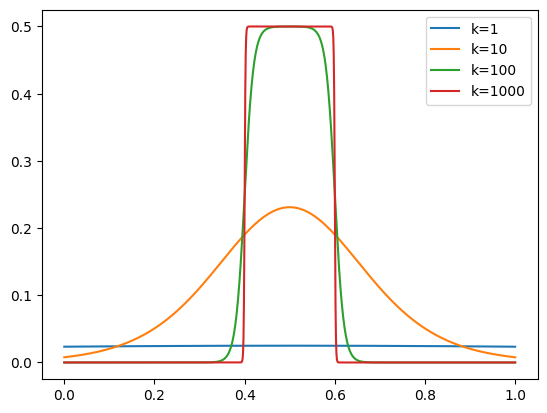
\includegraphics[scale=0.6]{img/bump_functions_1d.png}
      \caption{Bump function approximated with $a = 0.4, b = 0.6$, with differing values of $k$. } 
      \label{fig:bump_functions_1d}
    \end{figure}
  \end{example}

  \begin{example}[Bump Functions in $\mathbb{R}^2$]
    To do this for a 2-D step function, of the form 
    \begin{equation}
      f(x_1, x_2) = \begin{cases} 1 \text{ if } a < x_1 < b \\ 0 & \text{ if else} \end{cases}
    \end{equation}
    this is a simple extension of the first one. We just don't need to make our linear combination dependent on $x_2$ and we're done.
    \begin{equation}
      f(x) \approx \frac{1}{2} \sigma \big( k( x_1 - a)\big) - \frac{1}{2} \sigma \big( k (x_1 - b) \big)
    \end{equation}
  \end{example} 

  \begin{example}[Tower Functions in $\mathbb{R}^2$] 
    Now to construct a tower function of the form 
    \begin{equation}
      f(x_1, x_2) = \begin{cases} 1 & \text{ if } a_1 < x_1 < b_1, a_2 < x_2 < b_2 \\ 0 & \text{ if else} \end{cases}
    \end{equation}
    we need slightly more creativity. Now we can approximate it by doing 
    \begin{equation}
      f(x) \approx \sigma \bigg( k_2 \big[ \sigma\big( k_1 (x_1 - a_1)\big) - \sigma\big( k_1 (x_1 -b_1)\big) + \sigma \big( k_1 (x_2 - a_2)\big) - \sigma\big(k_1 (x_2 - b_2)\big)  big] - b_2\bigg)
    \end{equation}
  \end{example} 

  At this point, we can see how this would extend to $\mathbb{R}^n$, and by isolating parts of the network we can have it approximate tower functions that are completely separate from each other, at any height, and then finally take a linear combination of them to approximate the original function of interest.  

  \begin{theorem}[CS671 Fall 2023 PS5]
    Suppose you have a 2D, $L$-lipschitz function $f(x_1, x_2)$ defined on a unit square ($x_1, x_2 \in \left [0,1 \right ]$). You want to approximate this with an arbitrary neural net $\Tilde{f}$ such that
    \begin{equation}
      \sup_{x \in [0, 1]^2} |f(x) - \Tilde{f}(x)| \leq \epsilon
    \end{equation}
    If we divide the square into a checkerboard of $K \times K$ nonoverlapping squares, approximate the restriction of $f$ to each subsquare with a tower function, what is the least $K$ we would need to ensure that the error is less than $\epsilon$? 
  \end{theorem} 

\subsection{Parameter Symmetry}

  Early in the development of the theory of neural nets, An Mei Chen, (currently VP of engineering in Qualcomm) showed in \cite{symmetry} that for certain neural networks, there are multiple parameters $\theta$ that map to the same function $f$. 

  \begin{theorem}[Parameter Symmetry]
    Consider a 2-layer feedforward network of form 
    \begin{equation}
      f = W^{[2]} \circ \sigma \circ W^{[1]}
    \end{equation} 
    where $\sigma = \tanh$. Let $z$ be the hidden vector. We can see that by changing the signs of the $i$th row of $W^{[1]}$, $z_i$'s sign will be flipped. From the properties that $\tanh$ is an odd function (i.e. $\tanh(-x) = - \tanh(x)$), therefore the activation will be also sign-flipped, but this effect can be negated by flipping the $i$th column of the $W^{[2]}$. Therefore, given that $z \in R^{N}$, i.e there are $N$ hidden units, we can choose any set of row-column pairs of the weight matrices to invert, leading to a total of $2^N$ different weightings that produce the same function $f$. 

    Similarly, imagine that we permute the columns of $W^{[2]}$ and rows of $W^{[1]}$ in the same way. Then this will also lead to an invariance in $f$, and so this leads to $N! 2^N$ different weight vectors that lead to the same function! 
  \end{theorem}

\subsection{Smoothness} 

  Given that the input dimension is $D$, say that all the hidden layers are of dimension $D$ and we have $L$ layers. Then, we are storing a matrix (plus bias vector) at each layer, resulting in a scaling of $O(D^2 L)$. This quadratic scaling leads to overparameterized models, which should raise a red flag. This naturally leads to overfitting, but a strange phenomenon occurs.\footnote{I found this from Lex Fridman's podcast with Ilya Sutskever.}  
  \begin{enumerate}
    \item In the beginning, the training loss goes down along with the validation loss. 
    \item Soon the validation loss starts to go up while the training loss goes down, leading to overfitting. 
    \item The overfitting is worst when the training loss is $0$. 
    \item At this point, the training loss remains at $0$, but generalization starts to improve, and mysteriously the validation loss starts going down. 
  \end{enumerate}

  There are many theories of why the last step ever happens. To interpret this, let's revisit what overfitting means. It means that small perturbations of the inputs will result in large variances in the outputs. If we generalize well, $x + \epsilon$ should also result in $f(x) + O(\epsilon)$. Therefore, this means that the more parameters it has, the better this stability is and therefore the more robust the model. How should we measure this sense of stability? In analysis, a metric to assess the robustness of a deep neural net $f_\theta: \mathbb{R}^n \longrightarrow \mathbb{R}^m$ is its Lipshitz constant, which effectively bounds how much $f$ can change given some change in $x$. 

  \begin{definition}[Lipshitz Continuity]
    A function $f: \mathbb{R}^n \longrightarrow \mathbb{R}^m$ is called \textbf{Lipshitz continuous} if there exists a constant $L$ such that for all $x, y \in \mathbb{R}^n$
    \begin{equation}
      ||f(x) - f(y)||_2 \leq L ||x - y||_2
    \end{equation}
    and the smallest $L$ for which the inequality is true is called the \textbf{Lipshitz constant}, denoted $\mathrm{Lip}(f)$. 
  \end{definition}

  \begin{theorem}[Lipschitz Upper Bound with Operator Norm of Total Derivative]
    If $f: \mathbb{R}^n \longrightarrow \mathbb{R}^m$ is Lipschitz continuous, then 
    \begin{equation}
      \mathrm{Lip}(f) = \sup_{x \in \mathbb{R}^n} ||D_x f||_{\mathrm{op}}
    \end{equation}
    where $||\cdot ||_{\mathrm{op}}$ is the operator norm of a matrix. In particular, if $f$ is scalar-valued, then its Lipschitz constant is the maximum norm of its gradient on its domain 
    \begin{equation}
      \mathrm{Lip}(f) = \sup_{x \in \mathbb{R}^n} ||\nabla f(x)||_2
    \end{equation}
  \end{theorem}

  The above theorem makes sense, since indeed the stability of the function should be equal to the stability of its "maximum" linear approximation $D_x f$. 

  \begin{theorem}[Lipschitz Upper Bound for MLPs]
    It has already been shown that for a $K$-layer MLP
    \begin{equation}
      h_\theta (\mathbf{x}) \coloneqq \mathbf{T}_K \circ \boldsymbol{\rho}_{K-1} \circ \mathbf{T}_{K-1} \circ \cdots \circ \boldsymbol{\rho}_1 \circ \mathbf{T}_1 (\mathbf{x})
    \end{equation}
    the Lipshitz constant for an affine map $\mathbf{T}_k (\mathbf{x}) = M_k \mathbf{x} + b_k$ is simply the operator norm (largest singular value) of $M_k$, while that of an activation function is always bounded by some well-known constant, usually $1$. So, the Lipshitz constant of the entire composition $h$ is simply the product of all operator norms of $M_k$. 
  \end{theorem}

  What about $K$-computable functions in general? That is, given a function $f: \mathbb{R}^n \longrightarrow \mathbb{R}^m$ with 
  \begin{align}
    v_0 (\mathbf{x}) & = \mathbf{x} \\ 
    v_1 (\mathbf{x}) & = g_1 \big(v_0(\mathbf{x}) \big) \\
    v_2 (\mathbf{x}) & = g_2 \big(v_0(\mathbf{x}), v_1 (\mathbf{x}) \big) \\ 
    \ldots & = \ldots \\
    v_k (\mathbf{x}) & = g_k \big(v_0 (\mathbf{x}), v_1(\mathbf{x}), \ldots, v_{k-1} (\mathbf{x}) \big) \\
    \ldots & = \ldots \\
    v_K (\mathbf{x}) & = g_K \big(v_0(\mathbf{x}), v_1 (\mathbf{x}), \ldots, v_{K-2}(\mathbf{x}), v_{K-1}(\mathbf{x}) \big)
  \end{align}
  where $v_k: \mathbb{R}^n \longrightarrow \mathbb{R}^{n_k}$, with $n_0 = n$ and $n_K = m$, and 
  \begin{equation}
    g_k : \prod_{i=0}^{k-1} \mathbb{R}^{n_i} \longrightarrow \mathbb{R}^{n_k}
  \end{equation}
  To differentiate $v_k$ w.r.t. $\mathbf{x}$, we can use the chain rule, resulting in the total derivative 
  \begin{equation}
    \underbrace{\frac{\partial v_k}{\partial \mathbf{x}}}_{n_k \times n} = \sum_{i=1}^{k-1} \underbrace{\frac{\partial g_k}{\partial v_i}}_{n_k \times n_i} \, \underbrace{\frac{\partial v_i}{\partial \mathbf{x}}}_{n_i \times n}
  \end{equation}

  Therefore, it is this Lipschitz property that might entail how stable an MLP is. We have seen from the universal approximation theorems that for a data set of any size, we can always fit a one-layer perceptron that perfectly fits through all of them, given that the layer is large enough. In these cases, we are interested in fitting the data \textit{smoothly}, and theoretical research in bounding the Lipschitz constant is popular.

  In practice this behavior is reflected in \textit{most} cases, but they may be very sensitive in some cases, which we call \textit{adversarial examples}. Adversarial examples take advantage of this weakness by adding carefully chosen perturbations that drastically change the output of the network. Adversarial machine learning attempts to study these weaknesses and hopefully use them to create more robust models. It is natural to expect that the precise configuration of the minimal necessary perturbations is a random artifact of the normal variability that arises in different runs of backpropagation learning. Yet, it has been found that adversarial examples are relatively robust, and are shared by neural networks with varied number of layers, activations or trained on different subsets of the training data. This suggest that the deep neural networks that are learned by backpropagation have \textit{intrinsic} blind spots, whose structure is connected to the data distribution in a non-obvious way. 


\section{Autograd Engines}

  In numerical computing packages like \texttt{numpy} in Python and \texttt{eigen} in C++, we often work with scalars, vectors, and matrices. From linear algebra, the generalization of these objects is a tensor, which is an element of a tensor product space.\footnote{For a refresher, look at my linear algebra notes.} The full mathematical abstraction is rarely needed in practice, and so developers call tensors by their realization as \textit{multidimensional arrays}. 
  
  \begin{definition}[Tensor]
    A \textbf{tensor} is an element of a tensor product space $\bigotimes_i V_i$. It is represented as a \textbf{multidimensional array} of shape $(\dim(V_1), \ldots, \dim(V_n))$. 
  \end{definition}

  If we were trying to build a \texttt{Tensor} class from scratch, what attributes should it have? Well obviously we need the actual data in the tensor, which we will call \texttt{storage}, plus some metadata about the \texttt{shape} (in math, known as the tensor \textit{rank}). Usually, these packages optimize as much as possible for efficiency, and so these are implemented as C-style arrays, which then requires knowledge of the type of each element of the Tensor, called the \texttt{dtype}. Great, with these three attributes, we can do almost every type of arithmetic manipulation. Let's first introduce the most basic math tensor operations, which includes the normal operations supported in an algebra, plus some other ones. We will denote the shapes as well. 
  \begin{enumerate}
    \item \textit{Tensor Addition}. 
    \item \textit{Tensor Additive Inverse}. 
    \item \textit{Scalar Multiplication}. 
    \item \textit{Matrix Multiplication}. 
    \item \textit{Elementwise Multiplication}. 
    \item \textit{Elementwise Multiplicative Inverse}.  
    \item \textit{Transpose}. 
  \end{enumerate} 

  We would probably like some constructors that allows you to directly initialize tensors filled with $0$s (\texttt{zeros}), $1$s (\texttt{ones}), a multiplicative identity (\texttt{eye}\footnote{homophone for $I$, used to denoted the identity matrix.}) Some random initializers would be good, such as sampling from uniforms (\texttt{uniform}), \texttt{gaussians} (\texttt{gaussian}, \texttt{randn}). 

  Finally, we would like some very fundamental operations, such as typecasting, comparison, and indexing as well. 

  \begin{algorithm}[H]
    \caption{Tensor Class Implementation}
    \begin{algorithmic}[1]
    \State \textbf{class} Tensor:
        \State \textbf{Attributes:}
        \State \hspace{1em}storage: array  \Comment{Underlying data storage}
        \State \hspace{1em}shape: tuple    \Comment{Dimensions of tensor}
        \State \hspace{1em}dtype: type     \Comment{Data type of elements}

        \State \textbf{Constructors:}
        \State \texttt{def \_\_init\_\_(data, shape, dtype):}
            \State \hspace{2em}Initialize tensor with given data, shape, and dtype

        \State \textbf{Static Constructors:}
        \State \texttt{@staticmethod}
        \State \texttt{def zeros(shape, dtype):}
            \State \hspace{2em}\Return tensor filled with zeros
        \State \texttt{@staticmethod}
        \State \texttt{def ones(shape, dtype):}
            \State \hspace{2em}\Return tensor filled with ones
        \State \texttt{@staticmethod}
        \State \texttt{def eye(n, dtype):}
            \State \hspace{2em}\Return n×n identity matrix
        \State \texttt{@staticmethod}
        \State \texttt{def uniform(shape, low, high, dtype):}
            \State \hspace{2em}\Return tensor with uniform random values
        \State \texttt{@staticmethod}
        \State \texttt{def gaussian(shape, mean, std, dtype):}
            \State \hspace{2em}\Return tensor with gaussian random values

        \State \textbf{Arithmetic Operations:}
        \State \texttt{def \_\_add\_\_(self, other):}
            \State \hspace{2em}\Return element-wise addition
        \State \texttt{def \_\_neg\_\_(self):}
            \State \hspace{2em}\Return additive inverse
        \State \texttt{def \_\_mul\_\_(self, other):}
            \State \hspace{2em}\Return scalar or element-wise multiplication
        \State \texttt{def matmul(self, other):}
            \State \hspace{2em}\Return matrix multiplication
        \State \texttt{def \_\_truediv\_\_(self, other):}
            \State \hspace{2em}\Return element-wise division
        \State \texttt{def transpose(self):}
            \State \hspace{2em}\Return transposed tensor

        \State \textbf{Utility Operations:}
        \State \texttt{def \_\_repr\_\_(self):}
            \State \hspace{2em}\Return string representation
        \State \texttt{def \_\_str\_\_(self):}
            \State \hspace{2em}\Return human-readable string
        \State \texttt{def \_\_getitem\_\_(self, index):}
            \State \hspace{2em}\Return indexed value(s)
        \State \texttt{def \_\_eq\_\_(self, other):}
            \State \hspace{2em}\Return element-wise equality comparison
    \end{algorithmic}
  \end{algorithm}

  Note that there are other operations, such as concatenation, splitting, and stacking that would be a good idea to implement.  

\subsection{Strides} 

  A specific property of PyTorch is that they use strides as another source of metadata in storing tensors, which greatly speeds up operations. Consider that we want to transpose the first two dimensions of a tensor. Then, we would have to create a new tensor and fill it in with all the elements, which may be too computationally expensive for such a small operation. 

  \begin{definition}[Stride] 
    Given a tensor $T$ of size $(N_1, \ldots N_M)$, it is stored as a contiguous array of $\prod_m T_m$ elements, and we can index it as 
    \begin{equation}
      T[n_1, n_2, \ldots, n_M], \;\;\; 1 \leq n_i \leq N_i
    \end{equation} 
    To counteract this, the \textbf{stride} is a array $S$ of $M$ elements, 
    \begin{equation}
      S = (S_1, \ldots, S_M)
    \end{equation} 
    where indexing with some $I = (n_1, \ldots, n_M)$ is equivalent to computing $S \cdot I$ and taking that index in the array in memory. It defines a mapping. 
  \end{definition}

  If we do some calculation, the default stride of such a vector is defined 
  \begin{equation}
    S_m = \prod_{m < j} N_j, \;\;\; S_M = 1
  \end{equation}

  \begin{example}[Transposing]
    If we want to transpose the tensor above, then we change the stride from 
    \begin{equation}
      S = \bigg( \prod_{1 < j} N_j , \prod_{2 < j} N_j, \ldots, 1 \bigg)
    \end{equation} 
    to 
    \begin{equation}
      S = \bigg( \prod_{2 < j} N_j , \prod_{1 < j} N_j, \ldots, 1 \bigg)
    \end{equation} 
  \end{example}

\subsection{Automatic Differentiation} 

  \begin{lemma}[Derivative of $+/-$]
    Given two tensors $X, Y$ and $Z_+ = X + Y, Z_{-} = X - Y$, we have 
    \begin{align}
      \frac{\partial Z_+}{\partial X} = +1 && \frac{\partial Z_+}{\partial Y} = +1 \\ 
      \frac{\partial Z_-}{\partial X} = +1 && \frac{\partial Z_-}{\partial Y} = -1 
    \end{align}
    where $\pm1$ are tensors of $1$ or $-1$s of the same shape as $X, Y$. 
  \end{lemma}

  \begin{lemma}[Derivative of Element-wise Multiplication]
    Given two tensors $X, Y$ and $Z = X \odot Y$, we have 
    \begin{align}
      \frac{\partial Z}{\partial X} = Y && \frac{\partial Z}{\partial Y} = X
    \end{align}
  \end{lemma} 

  \begin{lemma}[Derivative of Matrix Multiplication]
    Given $X \in (N, M)$ and $Y \in (M, P)$, with $Z = XY \in (N, P)$, the derivative of matrix multiplication is 
    \begin{align}
      \frac{\partial Z}{\partial X} \in (N, P, N, M) && \bigg( \frac{\partial Z}{\partial X} \bigg)_{i, j, k, l} \coloneqq \frac{\partial Z_{i, j}}{\partial X_{k, l}} \\
      \frac{\partial Z}{\partial Y} \in (N, P, M, P) && \bigg( \frac{\partial Z}{\partial Y} \bigg)_{i, j, k, l} \coloneqq \frac{\partial Z_{i, j}}{\partial Y_{k, l}} 
    \end{align} 
  \end{lemma} 


\section{Weight Initialization}

  The way that we initialize our weights can have a huge impact on our training performance. Imagine that you are creating the first neural network and you want to decide how to initialize it. You may consider many different cases. 

  \begin{example}[Constant Initialization]
    You may first think of initializing everything to $0$ or $1$, which is the simplest. Let's run this, but we can already see by epoch 15 that we have some problems. 
    \begin{center}
      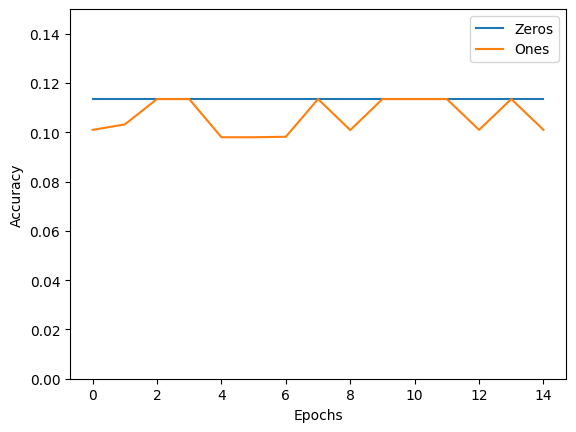
\includegraphics[scale=0.5]{img/first_initialize.png}
    \end{center}
    Clearly, this is not good, and theoretically this makes sense since it means all our activations are going to be the same, and thus all our gradients will be the same, meaning that are updates will be the same for every weight, which is not good mixing. We can see this below: 
  \end{example}

  \begin{example}[Random Initialization with High Variance]
    Okay, this didn't work, so perhaps you think it would be a good idea have more randomness to the initialization so that all the weights aren't exactly one number. You could think of initializing everything with three distinct schemes: 
    \begin{enumerate}[itemsep=0mm] 
      \item Randomly initialize everything to be $-1$ or $1$ with equal probability. 
      \item Randomly initialize everything to be a Gaussian random variable with standard deviation $1$. 
      \item Randomly initialize everything to be a uniform random variable between $-1$ and $1$. 
    \end{enumerate}
    Running the experiments give the following. 
    \begin{center} 
      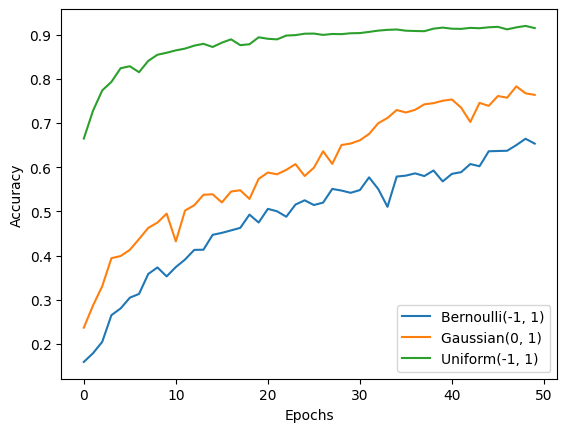
\includegraphics[scale=0.5]{img/second_initialization.png}
    \end{center}
    However, this is also not good since it means that the activations will be very large, and thus the gradients will be very large, and so the updates will be very large. This is not good since it means that the weights will be jumping around a lot, and we won't be able to converge. Furthermore, depending on what activations we choose, e.g. tanh or sigmoid, very large activations may saturate the gradients and kill the learning. 
  \end{example}

  \begin{example}[Random Initialization with Low Variance]
    This improves the next problem but now you want to fix the situation of the gradients being too big. Therefore, you should initialize the parameters to be smaller values, but not so small that they are zeros and we have the same problem as before. We use improved schemes: 
    \begin{enumerate}[itemsep=0mm] 
      \item Randomly initialize everything to be $-0.1$ or $0.1$ with equal probability. 
      \item Randomly initialize everything to be a Gaussian random variable with standard deviation $0.1$. 
      \item Randomly initialize everything to be a uniform random variable between $-0.1$ and $0.1$.
    \end{enumerate}
    \begin{center}
      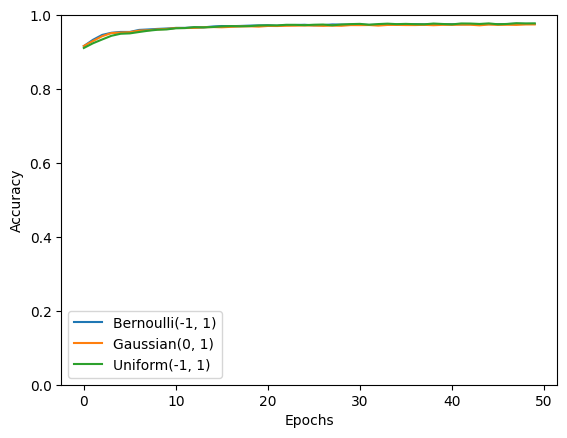
\includegraphics[scale=0.5]{img/third_initialize.png}
    \end{center}
  \end{example}

  Through out experiments, we have learned that a good rule of thumb for initializing weights is to make them small and uniformly random without being too small. While it is harder to get better than this for MNIST, a slightly better approach is Xavier initialization, which builds upon our same ideas. 

  \begin{definition}[Xavier Initialization]
    The \textbf{Xavier initialization} simply initializes each weight as a uniform distribution, with its range dependent on the size of the input. 
    \begin{equation}
      w_{ij}^{[l]} \sim U \bigg( -\frac{1}{\sqrt{N^{[l-1]}}}, \frac{1}{\sqrt{N^{[l-1]}}} \bigg)
    \end{equation}
    where $N^{[l-1]}$ is the number of neurons in the previous layer. This is a good rule of thumb for the weights, but the biases can be initialized to $0$ (though they are also initialized uniformly by default).
  \end{definition}

  \begin{code}[Experimenting with Weight Initializations] 
    The code used for generating the figures can be found \href{code/initialization.ipynb}{here}. 
  \end{code}


\section{Activation Functions} 

  The choice of the activation function can have a significant impact on your training, and we will describe a few examples below. The first thing to note is that we must ensure that there is a nonzero gradient almost everywhere. If, for example, we had a piecewise constant activation function, the gradient is $0$ almost everywhere, and it would kill the gradient of the entire network. In the early days of deep learning, researchers used the probability-inspired sigmoid and tanh functions as the main source of nonlinearity. Let's go over them below. 

  \begin{definition}[Sigmoid]
    Sigmoid activations are historically popular since they have a nice interpretation as a saturating ``fire rate" of a neuron. However, there are 3 problems: 
    \begin{enumerate}
      \item The saturated neurons ``kill" the gradients, since if the input at any one point in the layers is too positive or negative, the gradient will vanish, making very small updates. This is known as the \textbf{vanishing gradient problem}. Therefore, the more layers a neural network has, the more likely we are to see this vanishing gradient problem. 
      \item Sigmoid functions are not zero centered (i.e. its graph doesn't cross the point $(0, 0)$ ). Consider what happens when the input $x$ to a neuron is always positive. Then, the sigmoid $f$ will have a gradient of 
      \begin{equation}
        f \bigg( \sum_i w_i x_i + b \bigg) \implies \frac{\partial f}{\partial w_i} = f^\prime \bigg( \sum_i w_i x_i + b \bigg)\, x_i
      \end{equation}
      which means that the gradients $\nabla_\mathbf{w} f$ will always have all positive elements or all negative elements, meaning that we will be restricted to moving in certain nonoptimal directions when updating our parameters. 
    \end{enumerate}
  \end{definition} 

  \begin{definition}[Hyperbolic Tangent]
    The hyperbolic tangent is zero centered, which is nice, but it still squashes numbers to range $[-1, 1]$ and therefore kills the gradients when saturated. 
  \end{definition}

  It turns out that these two activations were ineffective in deep learning due to saturation. A less probability inspired activation was the ReLU, which showed better generalization an speed of convergence. 

  \begin{definition}[Rectified Linear Unit]
    The ReLU function has the following properties: 
    \begin{enumerate}
        \item It does not saturate in the positive region. 
        \item It is very computationally efficient (and the fact that it is nondifferentiable at one point doesn't really affect computations). 
        \item It converges much faster than sigmoid/tanh in practice. 
        \item However, note that if the input is less than $0$, then the gradient of the ReLU is $0$. Therefore, if we input a vector that happens to have all negative values, then the gradient would vanish and we wouldn't make any updates. These ReLU ``dead zones" can be a problem since it will never activate and never update, which can happen if we have bad initialization. A more common case is when your learning rate is too high, and the weights will jump off the data manifold. 
    \end{enumerate}
  \end{definition}

  Unfortunately, the ReLU had some weaknesses, mainly being the \textit{dying ReLU}, which is when the ReLU is stuck in the negative region and never activates. This is a problem since the gradient is $0$ in the negative region, and so the weights will never update. Therefore, some researchers have proposed some modifications to the ReLU. 

  \begin{definition}[Leaky ReLU]
    The leaky ReLU 
    \begin{equation}
      \sigma(x) = \max\{0.01 x, x\}
    \end{equation}
    does not saturate (i.e. gradient will not die), is computationally efficient, and converges much faster than sigmoid/tanh in practice. We can also parameterize it with $\alpha$ and have the neural net optimize $\alpha$ along with the weights. 
    \begin{equation}
      \sigma(x) = \max\{\alpha x, x\}
    \end{equation}
  \end{definition}

  \begin{definition}[ELU]
    The exponential linear unit has all the benefits of ReLU, with closer to mean outputs. It has a negative saturation regime compared with leaky ReLU, but it adds some robustness to noise. 
    \begin{equation}
      \sigma(x) = \begin{cases} x & \text{ if } x > 0 \\ \alpha \big(\exp{x} - 1 \big) & \text{ if } x \leq 0 \end{cases}
    \end{equation}
  \end{definition}

  \begin{definition}[SELU]
    The scaled exponential linear unit is a self-normalizing activation function, which means that it preserves the mean and variance of the input. This is useful for deep networks, since the mean and variance of the input will be preserved through the layers. Its formula is 
    \begin{equation}
      \sigma(x) = \lambda \begin{cases} x & \text{ if } x > 0 \\ \alpha \big(\exp{x} - 1 \big) & \text{ if } x \leq 0 \end{cases}
    \end{equation}
    where $\lambda$ and $\alpha$ are constants.
  \end{definition}
  
  Later on, some further modifications were made, such as the \textbf{Swish} and the \textbf{Mish} \cite{mish} activation functions. These functions have a distinctive negative concavity, unlike ReLU, which accounts for preservation of small negative weights.  

  \begin{definition}[Swish]
    The Swish activation function is defined as 
    \begin{equation}
      \sigma(x) = x \cdot \sigma(\beta x) 
    \end{equation}
    where $\beta$ is a parameter that can be learned. 
  \end{definition}

  \begin{definition}[Mish]
    The Mish activation function is defined as 
    \begin{equation}
      \sigma(x) = x \cdot \tanh(\ln(1 + \exp(x))) 
    \end{equation}
  \end{definition}

  \begin{code}[Generating Graphs] 
    Code used to generate these graphs are \href{code/activation_functions.ipynb}{here}.
  \end{code} 


\section{Popular Benchmark Datasets} 

  For here, we will go over some of the main datasets that are used in deep learning. 

  \begin{definition}[MNIST and Fashion MNIST]
    The MNIST dataset consists of 60k training images and 10k test images of handwritten digits. The Fashion MNIST dataset consists of 60k training images and 10k test images of clothing items. These are considered quite easy with the basic benchmarks: 
    \begin{enumerate} 
      \item Linear classifiers can reach past 90\% accuracy. 
      \item A 2 layer MLP can reach up to 97\% accuracy. 
      \item A CNN can reach up to 99\% accuracy. 
    \end{enumerate}
  \end{definition}

  \begin{definition}[CIFAR10 and CIFAR 100]
    The CIFAR10 dataset consists of 60k 32x32 color images in 10 classes, with 6k images per class. The CIFAR100 dataset consists of 60k 32x32 color images in 100 classes, with 600 images per class. These are considered quite hard with the basic benchmarks: 
    \begin{enumerate} 
      \item Linear classifiers can reach past 40\% accuracy. 
      \item A 2 layer MLP can reach up to 60\% accuracy. 
      \item A CNN can reach up to 80\% accuracy. 
    \end{enumerate}
  \end{definition}

  \begin{definition}[ImageNet]
    The ImageNet dataset, created at Stanford by Fei-Fei Li \cite{ImageNet}, consists of 1.2 million training images and 50k validation images in 1000 classes. This is considered very hard with the basic benchmarks. 
  \end{definition}

  Creating your own custom dataset with spreadsheets or images is easy.\footnote{https://pytorch.org/tutorials/beginner/data\_loading\_tutorial.html} Loading it to a dataloader that shuffles and outputs minibatches of data is trivial. However, when doing so, you should pay attention to a couple things. 
  \begin{enumerate} 
    \item Batch size: The dataloader stores the dataset (which can be several hundred GBs) in the drive, and extracts batches into memory for processing. You should set your batch sizes so that they can fit into the GPU memory, which is often smaller than the CPU memory. 
  \end{enumerate}


\section{Regularization} 

  Given a dataset with $D$ binary features, let $g(H, D)$ be the number of binary trees with depth at most $H$ (including root node), with the restriction that the trees may not split on some variable multiple times within a path to a leaf node. Then, $g$ can be defined recursively. 
  \begin{enumerate}
      \item First, if $H = 1$, then $g(H, D) = 1$ always since we are just creating the trivial binary tree of one node. 
      \item If $D = 0$, then there are no features to split on and therefore we just have the single node $g(H, D) = 1$. 
      \item If $H > 1$ and $D > 0$, then say that we start with a node. We can either make this a leaf node by not performing any splitting at all, or split on one of the $D$ variables. Then for each of the 2 nodes created on the split, we are now working with $D-1$ features and a maximum height of $H-1$ for each of the subtrees generated from the 2 nodes. 
  \end{enumerate}
  All this can be expressed as 
  \[g(H, D) = \begin{cases} 1 + D \, \big[ g(H - 1, D - 1) \big]^2 & \text{ if } H > 1, D > 0 \\ 1 & \text{ if } H = 1 \text{ or } D = 0 \end{cases} \]
  which is extremely large (in fact, NP hard). Therefore, some tricks like regularization must be implemented to limit our search space. 

  By defining the complexity of our decision tree $\Omega(h)$ as the number of nodes within the tree, we can modify our objective function to 
  \[L(h; \mathcal{D}) = \frac{1}{N} \sum_{i=1}^N 1_{\{y^{(i)} \neq h(x^{(i)})\}} + \lambda \Omega(h)\]
  We can impose this constraint directly on the training algorithm, or we can calculate the regularized loss after the tree has been constructed, which is a method called \textbf{tree pruning}. 

  Given a large enough $\lambda$, we can in fact greatly reduce our search space by not considering any trees further than a certain point. 

  \begin{theorem}
  We describe a tree as a set of leaves, where leaf $k$ is a tuple containing the logical preposition satisfied by the path to leaf $k$, denoted $p_k $, and the class label predicted by the leaf, denoted $\hat{y}_k$. For a dataset with $d$ binary features, $p_k: \{0, 1\}^d \to \{0, 1\}$ is a function that returns $1$ if a sample $x_i$ satisfies the preposition, and $0$ otherwise. That is, leaf $k$ is $(p_k, \hat{y}_k),$ and a tree $f$ with $K$ leaves is described as a set $f = \{(p_1, \hat{y}_1), \hdots, (p_K, \hat{y}_K)\}$. Assume that the label predicted by $\hat{y}_k$ is always the label for the majority of samples satisfying $p_k$. Finally, let $m_k = \sum_{i=1}^n p_k(x_i)$ denote the number of training samples ``captured'' by leaf $k$.

  Given a (potentially optimal) tree 

    \[f = \{(p_1, \hat{y}_1), \hdots, (p_{\kappa}, \hat{y}_{\kappa}), \hdots, (p_K, \hat{y}_K)\}, \]

  the tree $f' = \{(p_1, \hat{y}_1), \hdots, (p_{\kappa_1}, \hat{y}_{\kappa_1}), (p_{\kappa_2}, \hat{y}_{\kappa_2}), \hdots, (p_K, \hat{y}_K)\}$ produced by splitting leaf $(p_{\kappa}, \hat{y}_{\kappa})$ into two leaves $(p_{\kappa_1}, \hat{y}_{\kappa_1})$ and $(p_{\kappa_2}, \hat{y}_{\kappa_2})$ and any tree produced by further splitting $(p_{\kappa_1}, \hat{y}_{\kappa_1})$ or $(p_{\kappa_2}, \hat{y}_{\kappa_2})$ cannot  be optimal if $m_{\kappa} < 2n\lambda$.
  \end{theorem}
  \begin{proof}
  Let $c$ be the number of misclassifications in leaf $(p_{\kappa}, \hat{y}_{\kappa})$. Since a leaf classifies according to the majority of $m_{\kappa}$, we must have 

    \[c \leq \frac{m_\kappa}{2} < n \lambda\]

  By splitting leaf $(p_\kappa, \hat{y}_\kappa)$ into leaves $(p_{\kappa_1}, \hat{y}_{\kappa_1})$ and $(p_{\kappa_2}, \hat{y}_{\kappa_2})$, assume that we have reduced the number of misclassifications by $b \leq c$. Then, we have 

    \[\ell(f^\prime, \mathbf{X}, \mathbf{y}) = \ell(f, \mathbf{X}, \mathbf{y}) - \frac{b}{n}\]

  However, we have increased the number of leaves by $1$, and so 

    \[\lambda s(f^\prime) = \lambda s(f) + \lambda\]

  Combining the last two equations, we have obtained 

    \[R (f^\prime, \mathbf{X}, \mathbf{y}) = R(f, \mathbf{X}, \mathbf{y}) + \lambda - \frac{b}{n}\]

  However, we know that 

  \begin{align*}
    b \leq c & \implies \frac{b}{n} \leq \frac{c}{n} < \frac{n \lambda}{n} = \lambda \\
    & \implies - \frac{b}{n} > - \lambda \\
    & \implies \lambda - \frac{b}{n} > \lambda - \lambda = 0
  \end{align*}

  and so $R (f^\prime, \mathbf{X}, \mathbf{y}) > R(f, \mathbf{X}, \mathbf{y})$. This means that $f^\prime$ cannot be optimal according to our regularized objective. We have also proved that further splitting $(p_{\kappa_1}, \hat{y}_{\kappa_1})$ or $(p_{\kappa_2}, \hat{y}_{\kappa_2})$ cannot  be optimal since we can just set $f = f^\prime$, and apply the same argument. 
  \end{proof}

\subsection{Pruning} 

\subsection{Splitting} 

\section{Compression}

\subsection{Pruning}

  It can be computationally and memory intensive to train and utilize neural networks. This is where network pruning comes in, which attempts to identify a subnetwork that performs as well as the original. Given a neural net $f(\mathbf{x}, \boldsymbol{\theta})$ where $\boldsymbol{\theta} \in \mathbb{R}^M$, a pruned neural network can be thought of as a subnetwork $f(\mathbf{x}, \mathbf{m} \odot \boldsymbol{\theta})$, where $\mathbf{m}$ is a \textbf{mask}, i.e. a vector in $\{0, 1\}^M$ that, when multiplied component-wise to $\boldsymbol{\theta}$, essentially ``deletes" a portion of the parameters. 

  \begin{center}
    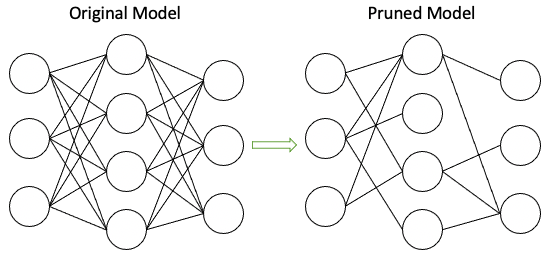
\includegraphics[scale=0.4]{img/pruned_network.png}
  \end{center}

  This idea has been around for a long time, and the general method of pruning is as such: 
  \begin{enumerate}
      \item We initialize the neural network $f(\mathbf{x}, \boldsymbol{\theta}_0)$ and train it until we have $f(\mathbf{x}, \boldsymbol{\theta})$. 
      \item We now prune the network. The most basic pruning scheme is to keep the top $k\%$ largest weights, since smaller weights do not contribute much to the forward prop, and thus can be ignored. 
  \end{enumerate}
  These pruned networks have been shown to reach accuracies as high as the original network, with equal training progress. Now, if we were to take only this pruned network and train it from the beginning, it will perform as well as the original network, \textit{only under} the condition that we start from the same initialization $\mathbf{m} \odot \boldsymbol{\theta}$. If we take this subnetwork and initialize it differently at $\boldsymbol{\theta}_0^\prime$, then this subnetwork would not train well. Therefore, the performance of the pruned network is dependent on the initialization! 

  If we had initialized the full network differently, trained it, and then pruned again, we may have a different subnetwork that will only train well on its own given this new initialization. Therefore, a good initialization is extremely important for training subnetworks. This fact doesn't help much since we can't just take some arbitrary subnetwork and train it since we don't know the good initialization. We must always train the full network, then find the subnetwork, and then find its initialization. 

  This is essentially the \textbf{lottery ticket hypothesis} \cite{lottery}, which states that a randomly-initialized, dense neural network contains a subnetwork that is initialized such that, when trained in isolation, it can match the test accuracy of the original network after training for at must the same number of iterations. 

  This paper hints at why neural networks work at all. It first states that only a very small subnetwork is responsible for the vast majority of its performance, but it must be initialized at the right position. But by overparameterizing these neural nets so much (by a certain margin), they have so many different combinations of subnetworks such that whatever initialization you throw at it, it is guaranteed that some subnetwork within it will train well with this initialization. This subnetwork is called the \textit{winning ticket}. 

\subsection{Quantization}


\section{Exercises} 

\subsection{Group Like Structures}

  \begin{exercise}[Math 401 Spring 2025 Midterm 2]
    Listed. 
    \begin{enumerate}
      \item Let $G$ be a finite group with an even number of elements. Show that $G$ contains an element of order $2$. 
      \item Prove that a group of order $10$ contains an element of order $5$. 
    \end{enumerate}
  \end{exercise}
  \begin{solution}
    Listed. 
    \begin{enumerate}
      \item We know that $e^{-1} = e$, and so remove it from $G$. Then $G$ has an odd number of elements. Now as long as $G$ is nonempty, we can remove $a, a^{-1}$, resulting in an odd cardinality. Since $G$ is finite, this must terminate, and so there must be a case where $a = a^{-1} \implies \ord(a) = 2$. 
      \item Assume that there is no element of order $5$. Then from above it must contain an element of order $2$, and let us call it $a \in G$. $\ord(e) = 1$ obviously. If any $b \in G$ had order 10, then $G = Z_{10}$, which would mean that $\ord(b^5) = 2$. Therefore every element other than the identity must have order $2$. But then given $a, b, ab \in G$, $ab \neq a, b$ since $ab = a \implies b = e$, and this is precisely the Klein 4 group. This subgroup has an order that doesn't divide 10, contradicting Lagrange's theorem. 
    \end{enumerate}
  \end{solution}

  \begin{exercise}[Shifrin 6.1.1]
    Which of the following are groups?
    \begin{enumerate}
      \item[(a)] $\{1,3,7,9\} \subset \mathbb{Z}_{10}$, with operation multiplication
      \item[(b)] $\{0,2,4,6\} \subset \mathbb{Z}_{10}$, with operation addition
      \item[(c)] $\{x \in \mathbb{Q} : 0 < x \leq 1\}$, with operation multiplication
      \item[(d)] the set of all positive irrational real numbers, with operation multiplication
      \item[(e)] the set of imaginary numbers $ix, x \in \mathbb{R}$, with operation addition
      \item[(f)] the set of complex numbers of modulus 1, with operation multiplication
      \item[(g)] $\mathbb{Z}$ with operation $a \bullet b = a + b + 1$
      \item[(h)] $\mathbb{Z}$ with operation $a \bullet b = a - b$
      \item[(i)] $\mathbb{Q} - \{1\}$ with operation $a \bullet b = a + b - ab$
    \end{enumerate}
  \end{exercise}
  \begin{solution}
    Listed. We will denote the sets in question to be $G$. 
    \begin{enumerate}
      \item[(a)] Is a group since product of 2 odds is odd, so is closed. Also we have $1$ as the identity with $3^{-1} = 7, 7^{-1} = 3, 9^{-1} = 9$. It is associative since multiplication on $\mathbb{Z}_{10}$ is associative. 
      \item[(b)] Not a group since $4 + 4 = 8 \not\in G$. 
      \item[(c)] Not a group since $1/2 \in G$ but $(1/2)^{-1} = 2 \not\in G$. 
      \item[(d)] Not a group since $\sqrt{2} \times \sqrt{2} 2  \not\in G$. 
      \item[(e)] Is a group since identity is $0 = 0i$, $ix + iy = i (x + y)$ with $x + y \in \mathbb{R}$, and $-(ix) = i (-x)$ where $-x \in \mathbb{R}$. 
      \item[(f)] Is a group since this is a representation of $O(2)$. 
      \item[(g)] Is a group since this is obviously closed under $\mathbb{Z}$ since $+_{\mathbb{Z}}$ is closed. Now assume that $i$ is the identity. Then $a \bullet i = a + i + 1 = a \implies i = -1$. Therefore $a \bullet a^{-1} = a + a^{-1} + 1 = -1 \implies a^{-1} = -a - 2$. This is associative since 
      \begin{equation}
        (a \bullet b) \bullet c = (a + b + 1) \bullet c = a + b + c + 2 = a \bullet (b + c + 1) = a \bullet (b \bullet c)
      \end{equation}
      \item[(h)] Not a group since it is not associative. Note $(a \bullet b) \bullet c = (a - b) \bullet c = a - b - c$, while $a \bullet (b \bullet c) = a \bullet (b - c) = a - b + c$. 
      \item[(i)] Is a group. We claim that it is closed. Assume not; given $a, b \neq 1$, 
        \begin{equation}
          a \bullet b = a + b - ab = 1 \implies 0 = ab - a - b + 1 = (a - 1)(b-1) 
        \end{equation}
        which means $a = 1$ or $b = 1$, which is a contradiction. As for the identity, $a \bullet i = a + i - ai = a \implies 0 = i - ai = i (1 - a) \implies i = 0$ since $a \neq 1$. We can define the inverse by solving 
        \begin{equation}
          0 = a \bullet a^{-1} = a + a^{-1} - a a^{-1} \implies a^{-1} (1 - a) = -a \implies a^{-1} = \frac{a}{a-1}
        \end{equation}
        which is well-defined since $a \neq 1$. Finally, it is associative since 
        \begin{align}
          (a \bullet b) \bullet c & = (a + b - ab) \bullet c \\
                                  & = a + b - ab + c - ac - bc - abc \\
                                  & = a + b + c - bc - ab - ac - abc \\
                                  & = a \bullet (b + c - bc) \\
                                  & = a \bullet (b \bullet c)
        \end{align}
    \end{enumerate}
  \end{solution}

  \begin{exercise}[Shifrin 6.1.10]
    \begin{enumerate}
      \item[(a)] Let $G$ be a group. Prove that $(ab)^2 = a^2b^2$ for all $a,b \in G$ if and only if $G$ is abelian.
      \item[(b)] Prove that if every element (other than the identity element) of a group $G$ has order 2, then $G$ is abelian.
    \end{enumerate}
  \end{exercise}
  \begin{solution}
    For (a), if $G$ is abelian, then 
    \begin{equation}
      (ab)^2 = (ab) (ab) = a (ba) b = a (ab) b = (aa) (bb) = a^2 b^2
    \end{equation}
    If the identity holds, then 
    \begin{equation}
      (ab)^2 = a^2 b^2 \implies (a^{-1} a) (ba) (b b^{-1}) = a^{-1} (ab)(ab) b^{-1} = a^{-1} a^2 b^2 b^{-1} \implies ba = ab
    \end{equation} 
    For (b), since we have $a^2 = e, b^2 = e$, and $(ab)^2 = e$, from (a) $G$ is abelian. 
  \end{solution}

  \begin{exercise}[Shifrin 6.1.17]
    \begin{enumerate}
      \item[(a)] A group has four elements $a$, $b$, $c$, and $d$, subject to the rules $ca = a$ and $d^2 = a$. Fill in the entire multiplication table at the left below.
      
      \begin{tabular}{c|cccc}
        $\cdot$ & $a$ & $b$ & $c$ & $d$ \\
        \hline
        $a$ & & & & \\
        $b$ & & & & \\
        $c$ & $a$ & & & \\
        $d$ & & & & $a$ \\
      \end{tabular}
      
      \item[(b)] A group has six elements $a$, $b$, $c$, $d$, $e$, and $f$, subject to the rules $ae = a$, $bd = a$, $c^2 = a$, and $df = a$. Fill in the entire multiplication table at the right above.
      
      \begin{tabular}{c|cccccc}
        $\cdot$ & $a$ & $b$ & $c$ & $d$ & $e$ & $f$ \\
        \hline
        $a$ & & & & & $a$ & \\
        $b$ & & & & $a$ & & \\
        $c$ & & & $a$ & & & \\
        $d$ & & & & & & $a$ \\
        $e$ & & & & & & \\
        $f$ & & & & & & \\
      \end{tabular}
    \end{enumerate}
  \end{exercise}
  \begin{solution}
    We can see that $ca = a \implies c = ca a^{-1} = a a^{-1} = i$, so $c$ is the identity. We can fill in the row and column of $c$. Then, we can figure out what $bd$ is. It cannot be $b$ or $d$ since $c$ is the unique identity, so it must be either $a$ or $c$. It cannot be $a$ since then $bd = a = d^2$, and so $b = d$. So it must be $c$. By the same logic we can fill out the rest of the rows and columns. 

    \begin{tabular}{c|cccc}
      $\cdot$ & $a$ & $b$ & $c$ & $d$ \\
      \hline
      $a$ & $c$ & $d$ & $a$ & $b$ \\
      $b$ & $d$ & $a$ & $b$ & $c$ \\
      $c$ & $a$ & $b$ & $c$ & $d$ \\
      $d$ & $b$ & $c$ & $d$ & $a$ \\
    \end{tabular}

    By the same logic as the previous, we can immediately see that $ae = a \implies e$ is the identity. The formal logic above can be simplified down to saying that there can be no two of the same elements in the same row or column, since if it were, then we are saying that $xy = xz \implies y = z$, which cannot be the case since $y$ and $z$ are distinct. So $fb = a$. We can also deduce that $da = ab$ and $ba = af$. At this point, we can recognize that this is the Dihedral group of order $6$, and so we fill in the rest of the multiplication table. 

    \begin{tabular}{c|cccccc}
      $\cdot$ & $a$ & $b$ & $c$ & $d$ & $e$ & $f$ \\
      \hline
      $a$ & c & f & e & b & a & d \\
      $b$ & d & e & f & a & b & c \\
      $c$ & e & d & a & f & c & b \\
      $d$ & f & c & b & e & d & a \\
      $e$ & a & b & c & d & e & f \\
      $f$ & b & a & d & c & f & e
    \end{tabular}
  \end{solution}

\subsection{Subgroups and Quotient Groups}

  \begin{exercise}[Shifrin 6.2.2]
    Prove that $\mathbb{Z}_7^{\times} \cong \mathbb{Z}_6$. (It is crucial to remember that we multiply in $\mathbb{Z}_7^{\times}$ and add in $\mathbb{Z}_6$.)
  \end{exercise}
  \begin{solution}
    Both groups are of order 6, and so $\mathbb{Z}_7^\times$---which is indeed a group (since it is the group of units of the ring $(\mathbb{Z}_7, +, \times)$)---must be isomorphic to either $\mathbb{Z}_6$ or $S_3$. However, $S_3$ is not abelian, while $\mathbb{Z}^\times_7$ is, so it must be the case that it is isomorphic to $\mathbb{Z}_6$. 
  \end{solution}

  \begin{exercise}[Shifrin 6.2.15.a/b]
    The \textbf{dihedral group} of order $2n$, denoted $\mathcal{D}_n$, is given by $\{\rho^i\psi^j : 0 \leq i < n, 0 \leq j \leq 1\}$ subject to the rules $\rho^n = e$, $\psi^2 = e$, and $\psi\rho\psi^{-1} = \rho^{-1}$.
    \begin{enumerate}
      \item Check this is really a group. That is, what is $(\rho^i\psi^j)^{-1}$, and what is the product $(\rho^i\psi^j)(\rho^k\psi^\ell)$?
      \item Check that $\mathcal{T} \cong \mathcal{D}_3$ and $S_q \cong \mathcal{D}_4$.
    \end{enumerate}
  \end{exercise}
  \begin{solution}
    We check the properties of a group. The following identity is useful: 
    \begin{equation}
      (\psi \rho \psi^{-1})^{n-i} = (\rho^{-1})^{n-i} \implies \psi \rho^{n-i} \psi^{-1} = \rho^i \implies \psi \rho^{n-i} = \rho^i \psi
    \end{equation}
    \begin{enumerate}
      \item \textit{Closure}. From simplifying according to the first two rules, we will automatically adjust the exponents to be $i, k < n$ (by subtracting out multiples of $n$) and $j \in \{0, 1\}$ (by subtracting out multiples of $2$). Going case by case, 
      \begin{enumerate}
        \item $j = 0, l = 0$. $\rho^i \rho^k = \rho^{i+k}$. 
        \item $j = 0, l = 1$. $\rho^i \rho^k \psi = \rho^{i+k} \psi$. 
        \item $j = 1, l = 0$. $\rho^i \psi \rho^k = \rho^i \rho^{n-k} \psi = \rho^{n-k+i} \psi$. 
        \item $j = 1, l = 1$. $\rho^i \psi \rho^k \psi = \rho^i \psi \psi \rho^{n-k} = \rho^i \rho^{n-k} = \rho^{n-k+i}$. 
      \end{enumerate}
      \item \textit{Identity}. The identity is $e = \rho^0 \psi^0$. We can see that $e \rho^i \psi^j = \rho^i \psi^j e = \rho^{i+0} \psi^j$. 
      \item \textit{Inverse}. We have $\psi \rho \psi^{-1} = \psi \rho \psi = \rho^{-1} \implies \psi \rho = \rho^{-1} \psi^{-1} = (\psi \rho)^{-1}$. Therefore, 
      \begin{equation}
        (\rho^i \psi^j)^{-1} = \begin{cases} 
          \rho^{n - i} & \text{ if } j = 0  \\
          \rho^{i} \psi & \text{ if } j = 1
        \end{cases}
      \end{equation}
      which are both of the correct form and therefore in $\mathcal{D}_n$. To verify, we see that $\rho^i \rho^{n-i} = \rho^n = e$, and $(\rho^i \psi) (\rho^i \psi) = \rho^i \psi \psi \rho^{n-i} = \rho^i \rho^{n-i} = e$.  
      \item \textit{Associativity}. Can also be proven tediously but problem only asked to state the product and inverse.  
    \end{enumerate} 

    For (b) for $\mathcal{T}$, we can explicitly look at the multiplication tables and see that they are isomorphic. We denote $r_1, r_2$ as the 120 and 240 degree rotations, and $f_1, f_2, f_3$ as the flips across each axis. 

    \begin{figure}[H]
      \centering
      \begin{subfigure}[b]{0.48\textwidth}
        \centering
        \begin{tabular}{c|cccccc}
          & $e$ & $\rho$ & $\rho^2$ & $\psi$ & $\rho\psi$ & $\rho^2\psi$ \\
          \hline
          $e$ & $e$ & $\rho$ & $\rho^2$ & $\psi$ & $\rho\psi$ & $\rho^2\psi$ \\
          $\rho$ & $\rho$ & $\rho^2$ & $e$ & $\rho^2\psi$ & $\psi$ & $\rho\psi$ \\
          $\rho^2$ & $\rho^2$ & $e$ & $\rho$ & $\rho\psi$ & $\rho^2\psi$ & $\psi$ \\
          $\psi$ & $\psi$ & $\rho^2\psi$ & $\rho\psi$ & $e$ & $\rho^2$ & $\rho$ \\
          $\rho\psi$ & $\rho\psi$ & $\psi$ & $\rho^2\psi$ & $\rho$ & $e$ & $\rho^2$ \\
          $\rho^2\psi$ & $\rho^2\psi$ & $\rho\psi$ & $\psi$ & $\rho^2$ & $\rho$ & $e$
        \end{tabular}
        \caption{$\mathcal{D}_3$}
      \end{subfigure}
      \hfill 
      \begin{subfigure}[b]{0.48\textwidth}
        \centering
        \begin{tabular}{c|cccccc}
          & $e$ & $r_1$ & $r_2$ & $f_1$ & $f_2$ & $f_3$ \\
          \hline
          $e$ & $e$ & $r_1$ & $r_2$ & $f_1$ & $f_2$ & $f_3$ \\
          $r_1$ & $r_1$ & $r_2$ & $e$ & $f_3$ & $f_1$ & $f_2$ \\
          $r_2$ & $r_2$ & $e$ & $r_1$ & $f_2$ & $f_3$ & $f_1$ \\
          $f_1$ & $f_1$ & $f_2$ & $f_3$ & $e$ & $r_2$ & $r_1$ \\
          $f_2$ & $f_2$ & $f_3$ & $f_1$ & $r_1$ & $e$ & $r_2$ \\
          $f_3$ & $f_3$ & $f_1$ & $f_2$ & $r_2$ & $r_1$ & $e$
        \end{tabular}
        \caption{$\mathcal{T}$}
      \end{subfigure}
    \end{figure}

    For $S_q$, it is tedious to write the full table, so we construct the isormorphisms using the generators. For $S_q$, the symmetry group of the square consists of 8 elements: the 4 rotations $r_1, r_2, r_3, r_4$ (of 90, 180, 270, and 360=0 degrees), and the flips $f_1, f_2, f_3, f_4$ (across each axis). Now we construct the function $g: \mathcal{D}_3 \rightarrow \mathcal{T}$ such that $f(\rho) = r_1$ and $f(\psi) = f_1$. Then we can see that 
    \begin{equation}
      g(\rho^4) = g(e) = e = r_1^4 = g(\rho^4), \qquad g(\psi^2) = g(e) = e = f_1^2 = g(\psi)^2
    \end{equation}
    since 90 degrees rotated 4 times is $0$ degrees, the identity, and two flips across the same axis is also the identity. Finally, we have 
    \begin{equation}
      g(\psi \rho \psi) = g(\rho^{-1}) = r_1^{-1} = r_3 = f_1 r_1 f_1 = g(\psi) g(\rho) g(\psi)
    \end{equation}
    Where $r_1^{-1} = r_3$ since a rotation of 270 after a 90 is the same as rotation by 360=0, and $r_3 = f_1 r_1 f_1$ is the change of basis symmetry observed in Shifrin Example 6.1.5. Therefore the rules match, making it a homomorphism, and since the order is the same ($\mathcal{D}_3$ has $4 \times 2 = 8$ elements from looking at the indices), this is an isomorphism. 
  \end{solution}

  \begin{exercise}[Shifrin 6.3.8]
    Let $H \subset G$ be a subgroup, and let $a \in G$ be given. Prove that $aHa^{-1} \subset G$ is a subgroup (called a \textbf{conjugate subgroup} of $H$). Prove, moreover, that it is isomorphic to $H$ (cf. Exercise 6.2.12).
  \end{exercise}
  \begin{solution}
    Let $x, y \in aHa^{-1}$. Then $x = a h_x a^{-1}, y = a h_y a^{-1}$ for some $h_x, h_y \in H$. Therefore, 
    \begin{enumerate}
      \item It is closed. $xy = (a h_x a^{-1}) (a h_y a^{-1}) = a h_x (a^{-1} a) h_y a^{-1} = a h_x h_y a^{-1} \in aHa^{-1}$ since $h_x h_y \in H$ by closure. 
      \item It has an identity since $e \in H \implies a e a^{-1} = a a^{-1} = e \in aHa^{-1}$. 
      \item It has inverses since given $x \in H$ as above with inverses $x^{-1}$, we see that $(a x a^{-1})^{-1} = (a^{-1})^{-1} x^{-1} a^{-1} = a x^{-1} a^{-1} \in a H a^{-1}$ since $x^{-1} \in H$ by $H$ being a group. 
      \item Associativity is inherited from $G$. 
    \end{enumerate} 
    It suffices to show that this is injective, since the map $\iota : H \rightarrow a H a^{-1}$ is surjective by definition. Given $x, y \in a H a^{-1}$ with $x = y$, we have $a h_x a^{-1} = a h_y a^{-1}$, and multiplying by $a$ on the right and then $a^{-1}$ on the left, we get $h_x = h_y$.
  \end{solution}

  \begin{exercise}[Shifrin 6.3.11]
    Prove that a group of order $n$ has a proper subgroup if and only if $n$ is composite.
  \end{exercise}
  \begin{solution}
    We prove bidirectionally. Call the group $G$ and subgroup $H$. 
    \begin{enumerate}
      \item $(\rightarrow)$. Assume $n$ is prime. Then by Lagrange's theorem $|H|$ must divide $n$, and so $|H| = 1$ or $n$, neither of which results in a proper subgroup. 
      \item $(\leftarrow)$. Assume $G$ has a proper subgroup $H$. Since it is proper, $|H| \neq 1, n$. Then by Lagrange's theorem, $|H|$ divides $n$, which implies that $n$ is composite. 
    \end{enumerate}
  \end{solution}

  \begin{exercise}[Shifrin 6.3.13]
    Suppose $H, K \subset G$ are subgroups of orders $5$ and $8$, respectively. Prove that $H \cap K = \{e\}$.
  \end{exercise}
  \begin{solution}
    Let us take an arbitrary element in $x \in H \cap K$ and consider the cyclic group $\langle x \rangle$. By Lagrange's Theorem, the order $|x|$ in $H$ must be either $1$ or $5$, while the order in $K$ must be $1, 2, 4, 8$. Therefore, $|x| = 1$ and so $x = e$. 
  \end{solution}

  \begin{exercise}[Shifrin 6.3.17]
    \begin{enumerate}
      \item Prove that a group $G$ of even order has an element of order $2$. (Hint: If $a \neq e$, $a$ has order $2$ if and only if $a = a^{-1}$.)
      \item Suppose $m$ is odd, $|G| = 2m$, and $G$ is abelian. Prove $G$ has precisely one element of order $2$. (Hint: If there were two, they would provide a Klein four-group.)
      \item Prove that if $G$ has exactly one element of order $2$, then it must be in the center of $G$.
    \end{enumerate}
  \end{exercise}
  \begin{solution}
    Listed. 
    \begin{enumerate}
      \item Assume the contrary and take $H = G \setminus \{e\}$. Then $|H|$ is odd, and since no element has order $2$, every element must be associated with a unique inverse $a, a^{-1}$. But this cannot happen since $|H|$ is odd. Therefore there must be at least one element of order $2$. 

      \item It has at least 1 element of order 2 from (1). Now assume that there are two, call them $a, b$. Then $ab \neq a, b$ and $ab$ also has order $2$ since $(ab)(ab) = abba = aa = e$. Therefore, calling $c = ab$, we have $ac = ca = aab = b$ and $bc = cb = abb = a$. This fully defines the multiplication table for the Klein 4 group $K$ of order $4$. Therefore, by Lagrange's theorem, we have found a subgroup $K$ and so $|K|$ must divide $G$. However, this would mean that $m$ must be even, a contradiction. Therefore there is only one such unique $a$. 

      \item Given $a \in G$ with $|a| = 2$, we wish to show that it is an element of $Z = \{ b \in G \mid bx = xb \forall x \in G\}$.\footnote{I am using the definition of center defined in Shifrin 6.3.7.} Consider $z = x^{-1} a x$. We have 
      \begin{equation}
        z^2 = (x^{-1} a x)^2 = x^{-1} a x x^{-1} a x = x^{-1} a^2 x = x^{-1} x = e
      \end{equation}
      which means that $z$ also has order $2$. But since this is unique, it must be that $z = a$. Therefore, by multiplying $x$ on the left, we get 
      \begin{equation}
        x^{-1} a x = a \implies ax = xa
      \end{equation}
    \end{enumerate}
  \end{solution}
  
  \begin{exercise}[Assigned]
    Find all group homomorphisms $\mathbb{Z}_n \to \mathbb{Z}_m$. (Your answer will depend on $n$ and $m$.) 
  \end{exercise}
  \begin{solution}
    Given a homomorphism, $f$, we must have $f(0) = 0$. Let $f(1) = k$. Note that the value of $f(1) = k$ completely determines the homomorphism since the image of every other $l \in \mathbb{Z}_n$ is defined by 
    \begin{equation}
      f(l) = f(\underbrace{1 + \ldots + 1}_{l \text{ times}}) = \underbrace{k + \ldots + k}_{l \text{ times}}
    \end{equation}
    Since the image of $f$ must be a cyclic subgroup of $\mathbb{Z}_m$, we must satisfy 
    \begin{align}
      0 = f(0) & = f(\underbrace{1 + \ldots + 1}_{n \text{ times}}) \\
               & = \underbrace{k + \ldots + k}_{n \text{ times}} 
    \end{align}
    and so $m \mid nk$. Therefore, $k$ must be a multiple of $m/\gcd(n, m)$. So all homomorphisms are determined by the set 
    \begin{equation}
      \bigg\{ k = \frac{a m}{\gcd(n, m)} \; \bigg| \; a \in \mathbb{N}, 0 \leq k \leq m-1 \bigg\}
    \end{equation}
    which we can see ranges from $0 \leq a < \gcd(n, m)$, and so the total number of homomorphisms is $\gcd(n, m)$. Note that there is always the trivial homomorphism when $a = 0$, i.e. everything maps to $0$. For example, if we have $f: \mathbb{Z}_{14} \to \mathbb{Z}_{21}$, we have $k = 0, 3, 6, 9, 12, 15, 18$. 
  \end{solution}

\subsection{Group Actions}

\subsection{Product Groups}

\subsection{Ring Like Structures}

  \begin{exercise}[Shifrin 1.2.1]
    For each of the following pairs of numbers $a$ and $b$, find $d = \gcd(a,b)$ and express $d$ in the form $ma+nb$ for suitable integers $m$ and $n$.
    \begin{enumerate}
      \item[(a)] $14, 35$
      \item[(b)] $56, 77$
      \item[(c)] $618, 336$
      \item[(d)] $2873, 6643$
      \item[(e)] $512, 360$
      \item[(f)] $4432, 1080$
    \end{enumerate}
  \end{exercise}
  \begin{solution}
    Listed. 
    \begin{enumerate}
      \item $d = 7 = (-2) \cdot 14 + (1) \cdot 35$. 
      \item $d = 7 = (-4) \cdot 56 + 3 \cdot 77$. 
      \item $d = 6 = -25 \cdot 618 + 46 \cdot 336$ 
      \item $d = 13 = 37 \cdot 2873 + (-16) \cdot 6643$. 
      \item $d = 8 = 19 \cdot 512 + (-27) \cdot 360$. 
      \item $d = 8 = 29 \cdot 4432 + (-119) \cdot 1080$. 
    \end{enumerate}
  \end{solution}

  \begin{exercise}[Shifrin 1.2.2]
    You have at your disposal arbitrarily many 4-cent stamps and 7-cent stamps. What are the postages you can pay? Show in particular that you can pay all postages greater than 17 cents.
  \end{exercise}

  \begin{exercise}[Shifrin 1.2.3]
    Prove that whenever $m \neq 0$, $\gcd(0, m) = |m|$.
  \end{exercise}

  \begin{exercise}[Shifrin 1.2.4]
    \begin{enumerate}
      \item[(a)] Prove that if $a|x$ and $b|y$, then $ab|xy$.
      \item[(b)] Prove that if $d = \gcd(a, b)$, then $\gcd(\frac{a}{d}, \frac{b}{d}) = 1$.
    \end{enumerate}
  \end{exercise}

  \begin{exercise}[Shifrin 1.2.5]
    Prove or give a counterexample: the integers $q$ and $r$ guaranteed by the division algorithm, Theorem 2.2, are unique.
  \end{exercise}

  \begin{exercise}[Shifrin 1.2.6]
     Prove or give a counterexample. Let $a, b \in \mathbb{Z}$. If there are integers $m$ and $n$ so that $d = am + bn$, then $d = \gcd(a, b)$.
  \end{exercise}

  \begin{exercise}[Shifrin 1.2.7]
    Generalize Proposition 2.5: if $\gcd(m, c) = 1$ and $m|cz$, then prove $m|z$.
  \end{exercise}
  \begin{solution}
    Let $\mathrm{gcd}(m, c) = 1$ and $m | cz$. Then there exists $a, b \in \mathbb{Z}$ such that $am + bc = 1$. Multiply both sides of the equation by $z$ to get by the distributive property 
    \begin{equation}
      (am + bc) z = amz + bcz = z
    \end{equation} 
    $m | amz$ and $m | cz \implies m | bcz$. Therefore, the sum of the two, which is equal to $z$, must be divisible by $m$. Therefore $m | z$. 
  \end{solution}

  \begin{exercise}[Shifrin 1.2.8]
    Suppose $a, b, n \in \mathbb{N}$, $\gcd(a, n) = 1$, and $\gcd(b, n) = 1$. Prove or give a counterexample: $\gcd(ab, n) = 1$.
  \end{exercise}

  \begin{exercise}[Shifrin 1.2.9]
    Prove that if $p$ is prime and $p|(a_1 a_2 \ldots a_n)$, then $p|a_j$ for some $j$, $1 \leq j \leq n$. (Hint: Use Proposition 2.5 and induction.)
  \end{exercise}

  \begin{exercise}[Shifrin 1.2.10]
    Given a positive integer $n$, find $n$ consecutive composite numbers.
  \end{exercise}

  \begin{exercise}[Shifrin 1.2.11]
    Prove that there are no integers $m, n$ so that $(\frac{m}{n})^2 = 2$. (Hint: You may start by assuming $m$ and $n$ are relatively prime. Why? Then use Exercise 1.1.3.)
  \end{exercise}

  \begin{exercise}[Shifrin 1.2.12]
    Find all rectangles whose sides have integral lengths and whose area and perimeter are equal.
  \end{exercise}

  \begin{exercise}[Shifrin 1.2.13]
    Given two nonzero integers $a, b$, in analogy with the definition of $\gcd(a, b)$, we define the \textbf{least common multiple} $\operatorname{lcm}(a, b)$ to be the positive number $\mu$ with the properties:
    \begin{enumerate}
      \item[(i)] $a|\mu$ and $b|\mu$, and
      \item[(ii)] if $s \in \mathbb{Z}$, $a|s$ and $b|s \Rightarrow \mu|s$.
    \end{enumerate}
    Prove that
    \begin{enumerate}
      \item[(a)] if $\gcd(a, b) = 1$, then $\mu = ab$. (Hint: If $\gcd(a, b) = 1$, then there are integers $m$ and $n$ so that $1 = ma + nb$; therefore, $s = mas + nbs$.)
      \item[(b)] more generally, if $\gcd(a, b) = d$, then $\mu = ab/d$.
    \end{enumerate}
  \end{exercise}
  \begin{solution}
    Listed. 
    \begin{enumerate}
      \item We can simply verify the two properties. Since $\mu = ab$, $a | \mu$ and $b | \mu$ trivially by the existence of $b$ and $a$, respectively. As for the second property, let $s \in \mathbb{Z}$ exist such that $a | s$ and $b | s$. Since $a | s$, $s = xa$ for some $x \in \mathbb{Z}$. But since $b | s$, $b | xa$. Since $\mathrm{gcd}(a, b) = 1$ by assumption, the result in [Shifrin 1.2.7] tells us that $b | x$, i.e. there exists some $k \in \mathbb{Z}$ such that $x = kb$. Therefore $s = xa = kba = kab = k \mu$. By existence of $k$, $\mu | s$, and we are done. 
      \item Given $a, b$ with $\mathrm{gcd}(a, b) = d$, there exists some $a^\prime, b^\prime \in \mathbb{Z}$ s.t. $a = da^\prime, b = db^\prime$. We claim that $\mu = ab/d \coloneqq d a^\prime b^\prime$ is the lcm.\footnote{Since division isn't generally closed in the integers, I prefer to define $ab/d$ this way.} It is clear that $a | \mu$ and $b | \mu$ by the existence of integers $b^\prime$ and $a^\prime$, respectively. To prove the second property, let $s \in \mathbb{Z}$ with $a | s$ and $b | s$. Since $a | s \iff d a^\prime | s$, there must exist some $x \in \mathbb{Z}$ s.t. $s = d a^\prime x$. But since $b | s$, this means that $d b^\prime | s \iff d b^\prime | d a^\prime x \iff b^\prime | a^\prime x$. But $\mathrm{gcd}(a^\prime, b^\prime) = 1$ which follows from the definition of gcd, and so by [Shifrin 1.2.7] it must be the case that $b^\prime | x$, i.e. there exists some $k \in \mathbb{Z}$ s.t. $x = b^\prime k$. Substituting this back we have $s = d a^\prime b^\prime k = \mu k$, and by existence of $k$ it follows that $\mu | s$. Since it satisfies these 2 properties $\mu$ is the lcm. 
    \end{enumerate}
  \end{solution} 

  \begin{exercise}[Shifrin 1.2.14]
    See Exercise 13 for the definition of $\operatorname{lcm}(a, b)$. Given prime factorizations $a = p_1^{\mu_1} \cdots p_m^{\mu_m}$ and $b = p_1^{\nu_1} \cdots p_m^{\nu_m}$, with $\mu_i, \nu_i \geq 0$, express $\gcd(a, b)$ and $\operatorname{lcm}(a, b)$ in terms of $p_1,\ldots,p_m$. Prove that your answers are correct.
  \end{exercise}

  \begin{exercise}[Shifrin 1.3.8] 
    We see that in $\bmod{10}$, 
    \begin{align}
      3^{400} \equiv 9^{200} \equiv (-1)^{200} \equiv 1^{100} \equiv 1
    \end{align} 
    so the last digit is $1$. To get the last 2 digits, we use the binomial expansion and focus on the last 2 terms. 
    \begin{equation}
      3^{400} = 9^{200} = (10 - 1)^{200} = \ldots + \binom{200}{199} 10^1 (-1)^{199} + \binom{200}{200} (-1)^{200} 
    \end{equation}
    since every combination of the form $\binom{n}{k}$ is an integer and all the other terms have a factor of $10^2$, the expansion $\bmod{100}$ becomes 
    \begin{equation}
      3^{400} \equiv \binom{200}{199} 10^1 (-1)^{199} + \binom{200}{200} (-1)^{200} = 200 \cdot 10 \cdot (-1)^{199} + 1 \equiv 1 \pmod{100}
    \end{equation}
    and so the last two digits is $01$. To get the last digit of $7^{99}$, we see that in $\bmod{10}$, 
    \begin{equation}
      7^{99} \equiv 7^{96} \cdot 7^3 \equiv (7^4)^{24} \cdot 343 \equiv 2401^{24} \cdot 343 \equiv 1^{24} \cdot 3 \equiv 3
    \end{equation}
  \end{exercise}

  \begin{exercise}[Shifrin 1.3.10]
    We must show that 
    \begin{equation}
      n \equiv 0 \pmod{13} \iff n^\prime = \sum_{i=1}^k a_i 10^{i-1} + 4a_0 \equiv 0 \pmod{13}
    \end{equation} 
    We see that $n \equiv n + 39 a_0 \equiv 0 \pmod{13}$, and 
    \begin{align}
      n + 39 a_0 & = \sum_{i=0}^k 10^i a_i + 39 a_0 \\
                 & = \sum_{i=1}^k 10^i a_i + 40 a_0 \\
                 & = 10 \bigg( \sum_{i=1}^k 10^{i-1} a_i + 4 a_0 \bigg) \\
                 & = 10 n^\prime
    \end{align} 
    and so we have $n \equiv 10 n^\prime \pmod{13}$, and so $n^\prime \equiv 0 \pmod{13} \implies n \equiv 0 \pmod{13}$. Conversely, if $n \equiv 0 \pmod{13}$, then $4n \equiv 0 \pmod{13}$, but $4n \equiv 40 n^\prime$ and so $n^\prime \equiv 40 n^\prime \equiv 4n \equiv 0 \pmod{13}$. Therefore both implications are proven. 
  \end{exercise}

  \begin{exercise}[Shifrin 1.3.12]
    Suppose that $p$ is prime. Prove that if $a^2 \equiv b^2 \pmod{p}$, then $a \equiv b \pmod{p}$ or $a \equiv -b \pmod{p}$. 
  \end{exercise}
  \begin{solution}
    We have 
    \begin{align}
      a^2 \equiv b^2 \pmod{p} & \implies a^2 - b^2 \equiv 0 \pmod{p} \\
                              & \implies (a + b) (a - b) \equiv 0 \pmod{p}
    \end{align} 
    We claim that there are no zero divisors in $\mathbb{Z}_p$. If $mn \equiv 0 \pmod{p}$, then by definition this means $p | mn$, which implies that in the integers this must mean that $p | m$ or $p | n$.\footnote{Proposition 2.5} But since $m, n \not\equiv 0$, $p \not| n$ and $p \not| m$, arriving at a contradiction. Going back to our main argument, it must be the case that $a + b \equiv 0 \implies a \equiv -b$ or $a - b \equiv 0 \implies a \equiv b$.  
  \end{solution}

  \begin{exercise}[Shifrin 1.3.15]
    Let us assume that $n = a^2 + b^2 + c^2$ for some $a, b, c \in \mathbb{Z}$. Let us consider for each integer $z$, all the possible values of $z^2 \pmod{8}$. 
    \begin{align}
      z \equiv 0 & \implies z^2 \equiv 0 \pmod{8} \\
      z \equiv 1 & \implies z^2 \equiv 1 \pmod{8} \\
      z \equiv 2 & \implies z^2 \equiv 4 \pmod{8} \\
      z \equiv 3 & \implies z^2 \equiv 1 \pmod{8} \\
      z \equiv 4 & \implies z^2 \equiv 0 \pmod{8} \\
      z \equiv 5 & \implies z^2 \equiv 1 \pmod{8} \\
      z \equiv 6 & \implies z^2 \equiv 4 \pmod{8} \\
      z \equiv 7 & \implies z^2 \equiv 1 \pmod{8} 
    \end{align}
    Therefore, $a^2 + b^2 + c^2 \pmod{8}$ can take any values of the form 
    \begin{equation}
      x + y + z \pmod{8} \text{ for } x, y, z \in \{0, 1, 4\}
    \end{equation}
    Since addition is commutative, WLOG let $x \leq y \leq z$. We can just brute force search this. 
    \begin{enumerate}
      \item If $z = 0$, then $x = y = z = 0$ and $x + y + z = 0 \not\equiv 7$. 
      \item If $z = 1$, then we see 
      \begin{align}
        0 + 0 + 1 \equiv 1 \\ 
        0 + 1 + 1 \equiv 2 \\ 
        1 + 0 + 1 \equiv 2 \\ 
        1 + 1 + 1 \equiv 3 
      \end{align}
      \item If $z = 4$, then we see that 
        \begin{align}
          0 + 0 + 4 & \equiv 4 \\
          0 + 1 + 4 & \equiv 5 \\
          0 + 4 + 4 & \equiv 0 \\
          1 + 1 + 4 & \equiv 6 \\
          1 + 4 + 4 & \equiv 1 \\
          4 + 4 + 4 & \equiv 4
        \end{align}
    \end{enumerate}
    And so $a^2 + b^2 + c^2 \not\equiv 7 \pmod{8}$ for any $a, b, c \in \mathbb{Z}$. 
  \end{exercise}

  \begin{exercise}[Shifrin 1.3.20.a/b/g]
    For (a), 
    \begin{equation}
      3x \equiv 2 \pmod{5} \implies 6x \equiv 4 \pmod{5} \implies x \equiv 4 \pmod{5} 
    \end{equation}
    For (b), 
    \begin{align}
      6x + 3 \equiv 1 \pmod{10} & \implies 6x \equiv -2 \equiv 8 \pmod{10} \\
                                & \implies 10 | (6x - 8) \\
                                & \implies 5 | (3x - 4) \\
                                & \implies 3x \equiv 4 \pmod{5} \\
                                & \implies 3x \equiv 9 \pmod{5} \\
                                & \implies x \equiv 3 \pmod{5}
    \end{align}
    For (g), 
    \begin{align}
      15x \equiv 25 \pmod{35} & \implies 35 | (15x - 25) \\
                              & \implies 7 | (3x - 5) \\
                              & \implies 3x \equiv 5 \pmod{7} \\
                              & \implies 3x \equiv 12 \pmod{7} \\ 
                              & \implies x \equiv 4 \pmod{7}
    \end{align}
  \end{exercise}

  \begin{exercise}[Shifrin 1.3.21.b/c]
    For (b), we see that $4$ and $13$ are coprime with $-3 \cdot 4 + 1 \cdot 13 = 1$. Therefore, by the Chinese remainder theorem 
    \begin{equation}
      x \equiv 1 \cdot 1 \cdot 12 + (-3) \cdot 7 \cdot 4 \pmod{52} \implies x \equiv 33 \pmod{52}
    \end{equation}
    For (c), we solve the first two congruences $x \equiv 3 \pmod{4}$ and $x \equiv 4 \pmod{5}$. $4$ and $5$ are coprime with $-1 \cdot 4 + 1 \cdot 5 = 1$. Therefore, by CRT 
    \begin{equation}
      x \equiv -1 \cdot 4 \cdot 4 + 1 \cdot 5 \cdot 3 \pmod{20} \implies x \equiv -1 \pmod{20}
    \end{equation}
    Then we solve $x \equiv -1 \pmod{20}$ with the final congruence $x \equiv 3 \pmod{7}$. We see that $20$ and $7$ are coprime with $-1 \cdot 20 + 3 \cdot 7 = 1$. Therefore by CRT 
    \begin{equation}
      x \equiv -1 \cdot 20 \cdot 3 + 3 \cdot 7 \cdot -1 \pmod{140} \implies x \equiv 59 \pmod{140}
    \end{equation}
  \end{exercise}

  \begin{exercise}[Shifrin 1.3.25]
    We prove bidirectionally. 
    \begin{enumerate}
      \item Assume a solution exists for $cx \equiv b \pmod{m}$. Then $m | (cx - b)$, which means that there exists a $y \in \mathbb{Z}$ s.t. $my = cx - b \iff b = cx - my$. Since $d = \mathrm{gcd}(c, m)$, there exists $c^\prime, m^\prime \in \mathbb{Z}$ s.t. $c = d c^\prime$ and $m = d m^\prime$. So 
      \begin{equation}
        b = cx - my = d (c^\prime x - m^\prime y) \implies d | b
      \end{equation} 

    \item Assume that $d | b$. Then there exists a $b^\prime \in \mathbb{Z}$ s.t. $b = d b^\prime$, and we have 
    \begin{align}
      cx \equiv b \pmod{m} & \iff m | (cx - b) \\
                           & \iff d m^\prime | d (c^\prime x - b^\prime) \\
                           & \iff m^\prime | (c^\prime x - b^\prime) \\
                           & \iff c^\prime x \equiv b^\prime \pmod{m^\prime} 
    \end{align}
    Since $\mathrm{gcd}(c^\prime, m^\prime) = 1$\footnote{Since $\mathrm{gcd}(c, m) = d \implies$ that there exists a $y, z \in \mathbb{Z}$ s.t. $c y + m z = d$, and dividing both sides by $d$ guarantees the existence of $y, z$ satisfying $c^\prime y + m^\prime z = 1$, meaning that $\mathrm{gcd}(c^\prime, m^\prime) = 1$.}, by Shifrin Proposition 3.5 the equation $c^\prime x \equiv b^\prime \pmod{m^\prime}$ is guaranteed to have a solution, and working backwards in the iff statements gives us the solution for $cx \equiv b \pmod{m}$. 
    \end{enumerate}

    We have proved existence of a solution in $\bmod{(m/d) = m^\prime}$. Now we show uniqueness. Assume that there are two solutions $x \equiv \alpha$, $x \equiv \beta \pmod{m^\prime}$ with $\alpha \not\equiv \beta \pmod{m^\prime}$. Then, $x$ can be written as $x = k_\alpha m^\prime + \alpha$ and $x = k_\beta m^\prime + \beta$. But we see that 
    \begin{align}
      0 = x - x & = (k_\alpha m^\prime + \alpha) - (k_\beta m^\prime + \beta) \\
                & = m^\prime (k_\alpha - k_\beta) + (\alpha - \beta) \\
                & \equiv \alpha - \beta \pmod{m^\prime}
    \end{align}
    which implies that $\alpha \equiv \beta \pmod{m^\prime}$, contradicting our assumption that they are different in modulo. Therefore the solution must be unique. 
  \end{exercise}

  \begin{exercise}[Shifrin 1.4.1]
    For $\mathbb{Z}_7$. There are no zero divisors and the units are all elements. 
    \begin{equation}
      \begin{array}{c|ccccccc}
        \times & 0 & 1 & 2 & 3 & 4 & 5 & 6 \\
        \hline
        0 & 0 & 0 & 0 & 0 & 0 & 0 & 0 \\
        1 & 0 & 1 & 2 & 3 & 4 & 5 & 6 \\
        2 & 0 & 2 & 4 & 6 & 1 & 3 & 5 \\
        3 & 0 & 3 & 6 & 2 & 5 & 1 & 4 \\
        4 & 0 & 4 & 1 & 5 & 2 & 6 & 3 \\
        5 & 0 & 5 & 3 & 1 & 6 & 4 & 2 \\
        6 & 0 & 6 & 5 & 4 & 3 & 2 & 1
      \end{array}
    \end{equation}
    For $\mathbb{Z}_8$. The zero divisors are $2, 4, 6$. The units are $1, 3, 5, 7$. 
    \begin{equation}
      \begin{array}{c|cccccccc}
        \times & 0 & 1 & 2 & 3 & 4 & 5 & 6 & 7 \\
        \hline
        0 & 0 & 0 & 0 & 0 & 0 & 0 & 0 & 0 \\
        1 & 0 & 1 & 2 & 3 & 4 & 5 & 6 & 7 \\
        2 & 0 & 2 & 4 & 6 & 0 & 2 & 4 & 6 \\
        3 & 0 & 3 & 6 & 1 & 4 & 7 & 2 & 5 \\
        4 & 0 & 4 & 0 & 4 & 0 & 4 & 0 & 4 \\
        5 & 0 & 5 & 2 & 7 & 4 & 1 & 6 & 3 \\
        6 & 0 & 6 & 4 & 2 & 0 & 6 & 4 & 2 \\
        7 & 0 & 7 & 6 & 5 & 4 & 3 & 2 & 1
      \end{array} 
    \end{equation}
    For $\mathbb{Z}_{12}$. The zero divisors are $2, 3, 4, 6, 8, 9, 10$. The units are $1, 5, 7, 11$. 
    \begin{equation}
      \begin{array}{c|cccccccccccc}
        \times & 0 & 1 & 2 & 3 & 4 & 5 & 6 & 7 & 8 & 9 & 10 & 11 \\
        \hline
        0 & 0 & 0 & 0 & 0 & 0 & 0 & 0 & 0 & 0 & 0 & 0 & 0 \\
        1 & 0 & 1 & 2 & 3 & 4 & 5 & 6 & 7 & 8 & 9 & 10 & 11 \\
        2 & 0 & 2 & 4 & 6 & 8 & 10 & 0 & 2 & 4 & 6 & 8 & 10 \\
        3 & 0 & 3 & 6 & 9 & 0 & 3 & 6 & 9 & 0 & 3 & 6 & 9 \\
        4 & 0 & 4 & 8 & 0 & 4 & 8 & 0 & 4 & 8 & 0 & 4 & 8 \\
        5 & 0 & 5 & 10 & 3 & 8 & 1 & 6 & 11 & 4 & 9 & 2 & 7 \\
        6 & 0 & 6 & 0 & 6 & 0 & 6 & 0 & 6 & 0 & 6 & 0 & 6 \\
        7 & 0 & 7 & 2 & 9 & 4 & 11 & 6 & 1 & 8 & 3 & 10 & 5 \\
        8 & 0 & 8 & 4 & 0 & 8 & 4 & 0 & 8 & 4 & 0 & 8 & 4 \\
        9 & 0 & 9 & 6 & 3 & 0 & 9 & 6 & 3 & 0 & 9 & 6 & 3 \\
        10 & 0 & 10 & 8 & 6 & 4 & 2 & 0 & 10 & 8 & 6 & 4 & 2 \\
        11 & 0 & 11 & 10 & 9 & 8 & 7 & 6 & 5 & 4 & 3 & 2 & 1
      \end{array} 
    \end{equation}
  \end{exercise}

  \begin{exercise}[Shifrin 1.4.5.a/b/c]
    \begin{enumerate}
      \item Prove that $\gcd(a, m) = 1 \iff \bar{a} \in \mathbb{Z}_m$ is a unit.
      \item Prove that if $\bar{a} \in \mathbb{Z}_m$ is a zero-divisor, then $\gcd(a, m) > 1$, and conversely, provided $m \nmid a$.
      \item Prove that every nonzero element of $\mathbb{Z}_m$ is either a unit or a zero-divisor.
      \item Prove that in any commutative ring $R$, a zero-divisor cannot be a unit, and a unit cannot be a zero-divisor. Do you think c.\ holds in general?
    \end{enumerate}
  \end{exercise}
  \begin{solution}
    For (a), 
    \begin{enumerate}
      \item $(\rightarrow)$. If $\mathrm{gcd}(a, m) = 1$, then there exists $x, y \in \mathbb{Z}$ such that $ax + my = 1$. Taking the modulo on both sides gives $ax \equiv 1 \pmod{m}$, and therefore we have established the existence of $x \in \mathbb{Z}$, which implies the existence of $\bar{x} \in \mathbb{Z}_m$. 

      \item $(\leftarrow)$. If we have $a \in \mathbb{Z}$ and $\bar{a}$ is a unit, then there exists a $\bar{x} \in \mathbb{Z}_m$ s.t. $\bar{a} \bar{x} = \bar{1} \iff ax \equiv 1 \pmod{m}$, which means that $m | (1 - ax)$. So there exists an integer $y \in \mathbb{Z}$ s.t. $my = 1 - ax \iff ax + my = 1$. By Shifrin corollary 2.4 $a, m$ must be coprime. 
    \end{enumerate}

    For (b), 
    \begin{enumerate}
      \item ($\rightarrow$) Let $\bar{a} \in \mathbb{Z}_m$ be a zero-divisor. Then there exists $\bar{x} \neq \bar{0}$ in $\mathbb{Z}_m$ such that $\bar{a}\bar{x} = \bar{0}$. This means: $ax \equiv 0 \pmod{m}$, so $m \mid ax$, and  $m \nmid x$ (since $\bar{x} \neq \bar{0}$). Since $m \mid ax$ but $m \nmid x$, some prime factor of $m$ must divide $a$. This prime factor is then a common divisor of $a$ and $m$ greater than 1, so $\gcd(a,m) > 1$.

      \item ($\leftarrow$) Let $a \in \mathbb{Z}$, $m \in \mathbb{N}$ where $\gcd(a, m) = d > 1$ and $m \nmid a$. Then $a = a'd$ and $m = m'd$ for some $a', m' \in \mathbb{Z}$. Therefore, 
      \begin{equation}
        \bar{a} \bar{m'} = \overline{am'} = \overline{a'd m'} = \overline{a'm} = \bar{0}
      \end{equation}
      Also since $m \nmid a$, we have $\bar{a} \neq \bar{0}$, and since $m = m'd$, we have $m \nmid m'$ (since $m \nmid a \implies d \neq m$), so $\bar{m'} \neq \bar{0}$. Therefore $\bar{a}$ is a zero-divisor in $\mathbb{Z}_m$.
    \end{enumerate}

    For (c), let $a \in \mathbb{Z}_m$ be a nonzero element. Then it must be the case that $\mathrm{gcd}(a, m) = 1$ or $\mathrm{gcd}(a, m)  > 1$. In the former case, $a$ is a unit by (a), and in the latter case, $a \not\equiv 0 \implies m \nmid a$\footnote{By contrapositive $m \mid a \implies a \equiv 0 \pmod{m}$ is trivial.}, and so by (b) $a$ is a zero divisor. 
  \end{solution}

  \begin{exercise}[Shifrin 1.4.6.b/c/d]
    Prove that in any ring $R$:
    \begin{enumerate}
      \item $0 \cdot a = 0$ for all $a \in R$ (cf.\ Lemma 1.1);
      \item $(-1)a = -a$ for all $a \in R$ (cf.\ Lemma 1.2);
      \item $(-a)(-b) = ab$ for all $a,b \in R$;
      \item the multiplicative identity $1 \in R$ is unique.
    \end{enumerate}
  \end{exercise}
  \begin{solution} 
    For (a), note that $0 a = (0 + 0) \cdot a = 0a + 0a$ and by subtracting $0a$ from both sides, we have $0 = 0a$. Similarly, $a0 = a (0 + 0) = a0 + a0 \implies 0 = a0$. 
    For (b), 
    \begin{align}
      a + (-1) \cdot a & = 1 \cdot a + (-1) \cdot a && \tag{definition of $1$} \\
                       & = (1 + -1) \cdot a && \tag{left distributivity} \\
                       & = 0 \cdot a && \tag{definition of add inverse}\\
                       & = 0 && \tag{From (a)}
    \end{align}
    For (c), note that by right distributivity, 
    \begin{align}
      (-1) \cdot a + a & = (-1) \cdot a + 1 \cdot a && \tag{definition of $1$} \\
                       & = (-1 + 1) \cdot a && \tag{right distributivity} \\
                       & = a \cdot 0 && \tag{definition of add inverse}\\
                       & = 0 && \tag{From (a)}
    \end{align}
    Therefore, 
    \begin{align}
      (-a)(-b) & = (-1 \cdot a) (-1 \cdot b) && \tag{from (b)}\\
               & = -1 \cdot (a \cdot -1) \cdot b && \tag{associativity} \\
               & = -1 \cdot -a \cdot b && \tag{from (b)} \\
               & = -1 \cdot -1 \cdot a \cdot b && \tag{from (b)} \\
               & = (-1 \cdot -1) \cdot ab && \tag{associativity} \\
               & = 1ab && \tag{shown below}\\
               & = ab && \tag{definition of identity}
    \end{align} 
    where $(-1)(-1) = 1$ since by (b), $(-1)(-1) = -(-1)$. We know that $-(-1)$ is an additive inverse for $-1$ and so is $1$. Since the multiplicative identity is unique in a ring, $-(-1) = 1$.  We show uniqueness for (d). Let us have $1 \neq 1^\prime$. Then by definition of identity, 
    \begin{equation}
      1 = 1 1^\prime = 1^\prime 1 = 1^\prime
    \end{equation}
    which is a contradiction. 
  \end{solution}

  \begin{exercise}[Shifrin 1.4.10]
    \begin{enumerate}
      \item Prove that the multiplicative inverse of a unit $a$ in a ring $R$ is unique. That is, if $ab = ba = 1$ and $ac = ca = 1$, then $b = c$. (You will need to use associativity of multiplication in $R$.)
      
      \item Indeed, more is true. If $a \in R$ and there exist $b,c \in R$ so that $ab = 1$ and $ca = 1$, prove that $b = c$ and thus that $a$ is a unit.
    \end{enumerate}
  \end{exercise}
  \begin{solution}
    For (a), we see that 
    \begin{equation}
      c = 1c = (ab)c = (ba)c = b(ac) = b(ca) = b1 = b
    \end{equation} 
    For (b), we have  
    \begin{equation}
      b = 1b = (ca)b = c(ab) = c1 = c
    \end{equation}
  \end{solution}

  \begin{exercise}[Shifrin 1.4.13]
    Let $p$ be a prime number. Use the fact that $\mathbb{Z}_p$ is a field to prove that $(p-1)! \equiv -1 \pmod{p}$. (Hint: Pair elements of $\mathbb{Z}_p$ with their multiplicative inverses; cf. Exercise 1.3.12.). 
  \end{exercise}
  \begin{solution}
    For $p = 2$, the result is trivial. Now let $p > 2$ be a prime. Then since $\mathbb{F}$ is a field, every element $a \in \mathbb{F}$ contains a multiplicative inverse $a^{-1}$. We claim that the only values for which $a = a^{-1}$ is $1, p-1$. Assume that $a = a^{-1}$. Then 
    \begin{equation}
      a^2 = 1 \implies p|(a^2 - 1) \implies p | (a+1)(a-1)
    \end{equation}
    and since $p$ is prime, it must be the case that $p|a+1 \iff a \equiv -1 \pmod{p}$ or $p|a-1 \iff a \equiv 1 \pmod{p}$. Therefore, we are left to consider the $(p-3)$ elements: $2, \ldots, p-2$. Since inverses are unique and the inverses of inverses is the original element, we can partition these $p-2$ elements into $(p-3)/2$ pairs.\footnote{Since $p \neq 2$, $p$ is odd and therefore $p-3$ is even.} Let's call the set of pairs $K = \{(a, b)\}$ where $b = a^{-1}$. Therefore, by commutativity and associativity we have 
    \begin{equation}
      (p-1)! \equiv (1)(p-1) \prod_{(a, b) \in K} ab \equiv -1 \cdot \prod_{(a, b) \in K} 1 \equiv -1 \pmod{p}. 
    \end{equation}
  \end{solution} 

  \begin{exercise}[Shifrin 2.3.2.a/b/c]
    Recall that the conjugate of the complex number $z = a + bi$ is defined to be $\bar{z} = a - bi$. Prove the following properties of the conjugate:
    \begin{enumerate}
      \item $\overline{z + w} = \bar{z} + \bar{w}$
      \item $\overline{zw} = \bar{z}\bar{w}$
      \item $\bar{z} = z \iff z \in \mathbb{R}$ and $\bar{z} = -z \iff iz \in \mathbb{R}$
      \item If $z = r(\cos\theta + i\sin\theta)$, then $\bar{z} = r(\cos\theta - i\sin\theta)$
    \end{enumerate}
  \end{exercise}
  \begin{solution}
    Let $z = a + bi, w = c + di$. For (a), 
    \begin{equation}
      \overline{z + w} = \overline{(a + c) + (b + d)i} = (a + c) - (b + d)i = a + c - bi - di = (a - bi) + (c - di) = \overline{z} + \overline{w}
    \end{equation} 
    For (b), 
    \begin{equation}
      \overline{zw} = \overline{(ac - bd) + (ad + bc)i} = (ac - bd) - (ad + bc)i = ac - bd - adi - bci = (a - bi)(c - di) = \bar{z}\bar{w}
    \end{equation}
    For (c), consider 
    \begin{align}
      \overline{z} = z & \iff a + bi = a - bi \\
                       & \iff bi = -bi \\
                       & \iff 2bi = 0 \\
                       & \iff b = 0 && \tag{field has no 0 divisors}
    \end{align}
    Therefore, $z = a \in \mathbb{R}$. 
    \begin{align}
      \overline{z} = -z & \iff a - bi = -a - bi \\
                        & \iff a = -a \\
                        & \iff 2a = 0 \\
                        & \iff a = 0 && \tag{field has no 0 divisors.}
    \end{align}
    Therefore, $z = bi \implies iz = -b \in \mathbb{R}$. 
  \end{solution}

  \begin{exercise}[Shifrin 2.3.3.a/b/c]
    Recall that the modulus of the complex number $z = a + bi$ is defined to be $|z| = \sqrt{a^2 + b^2}$. Prove the following properties of the modulus:
    \begin{enumerate}
      \item $|zw| = |z||w|$
      \item $|\bar{z}| = |z|$
      \item $|z|^2 = z\bar{z}$
      \item $|z + w| \leq |z| + |w|$ (This is called the triangle inequality; why?)
    \end{enumerate}
  \end{exercise}
  \begin{solution}
    Let $z = a + bi$ and $w = c + di$. For (a),
    \begin{align*}
      |zw| &= |(ac - bd) + (ad + bc)i| \\
      &= \sqrt{(ac - bd)^2 + (ad + bc)^2} \\
      &= \sqrt{a^2c^2 - 2abcd + b^2d^2 + a^2d^2 + 2abcd + b^2c^2} \\
      &= \sqrt{(a^2 + b^2)(c^2 + d^2)} \\
      &= \sqrt{a^2 + b^2}\sqrt{c^2 + d^2} \\
      &= |z||w|
    \end{align*}

    For (b), if $z = a + bi$, then $\bar{z} = a - bi$, so:
    \begin{equation}
      |\bar{z}| = \sqrt{a^2 + (-b)^2} = \sqrt{a^2 + b^2} = |z|
    \end{equation}

    For (c),
    \begin{align*}
      z\bar{z} &= (a + bi)(a - bi) \\
      &= a^2 + b^2 \\
      &= |z|^2
    \end{align*}
  \end{solution}

  \begin{exercise}[Shifrin 3.1.2.c/d]
    Find the greatest common divisors $d(x)$ of the following polynomials $f(x), g(x) \in F[x]$, and express $d(x)$ as $s(x)f(x) + t(x)g(x)$ for appropriate $s(x), t(x) \in F[x]$:
    \begin{enumerate}
      \item $f(x) = x^3 - 1$, $g(x) = x^4 + x^3 - x^2 - 2x - 2$, $F = \mathbb{Q}$
      \item $f(x) = x^2 + (1 - \sqrt{2})x - \sqrt{2}$, $g(x) = x^2 - 2$, $F = \mathbb{R}$
      \item $f(x) = x^2 + 1$, $g(x) = x^2 - i + 2$, $F = \mathbb{C}$
      \item $f(x) = x^2 + 2x + 2$, $g(x) = x^2 + 1$, $F = \mathbb{Q}$
      \item $f(x) = x^2 + 2x + 2$, $g(x) = x^2 + 1$, $F = \mathbb{C}$
    \end{enumerate}
  \end{exercise}
  \begin{solution}
    For (c), the gcd is $1$, with 
    \begin{equation} 
      -\frac{1}{1 - i} (x^2 + 1) + \frac{1}{1 - i} (x^2 - i + 2) = \frac{1}{1-i} (x^2 - i + 2 - x^2 - 1) = \frac{1}{1-i} (1 - i) = 1
    \end{equation}
    where $1/(1-i) = (1 + i)/2$. For (d), the gcd is $1$, with 
    \begin{align}
      \frac{1}{5} (2x + 3) (x^2 + 1) & + \frac{1}{5} (1 - 2x) (x^2 + 2x + 2) \\
                                          & = \frac{1}{5} (2x^3 + 3x^2 + 2x + 3) + \frac{1}{5} (-2x^3 - 3x^2 - 2x + 2) = 1
    \end{align}
  \end{solution}

  \begin{exercise}[Shifrin 3.1.6]
    Prove that if $F$ is a field, $f(x) \in F[x]$, and $\mathrm{deg}(f(x)) = n$, then $f(x)$ has at most $n$ roots in $F$. 
  \end{exercise}
  \begin{solution}
    We start when $n=1$. Then $f(x) = mx + b$ and we claim that the only root is $x = -b/m$ since we can solve for $0 = mx + b$ with the field operations, which leads to a unique solution. This implies by corr 1.5 that $(x + b/m)$ is the only factor of $f$. Now suppose this holds true for some degree $n-1$ and let us have a degree $n$ polynomial $f$. Assume that some $c$ is a root of $f$ (if there exists no $c$, then we are trivially done), which means $(x - c)$ is a factor of $f$, and we can write 
    \begin{equation}
      f(x) = (x - c) \, g(x)
    \end{equation}
    for some polynomial $g(x)$ of degree $n-1$. By our inductive hypothesis, $g(x)$ must have at most $n-1$ roots, and so $f$ has at most $n$ roots. 
  \end{solution}

  \begin{exercise}[Shifrin 3.1.8]
    Let $F$ be a field. Prove that if $f(x) \in F[x]$ is a polynomial of degree $2$ or $3$, then $f(x)$ is irreducible in $F[x]$ if and only if $f(x)$ has no root in $F$.
  \end{exercise}
  \begin{solution}
    We prove bidirectionally. 
    \begin{enumerate}
      \item $(\rightarrow)$. Let $f$ be irreducible. Then it cannot be factored into polynomials $p(x) q(x)$ where $\mathrm{deg}(p) + \mathrm{deg}(q) = n$. Note that two positive integers adding up to $2$ or $3$ means that at least one of the integers must be $1$, by the pigeonhole principle. This means that $f$ irreducible is equivalent to saying that $f$ does not have linear factors of form $(x-c)$, which by corollary 1.5 implies that there exists no root $c$ for $f(x)$. 
      \item $(\leftarrow)$. Let $f$ have no root in $F$. Then by corollary 1.5 there exists no linear factors $(x-c)$. By the same pigeonhole principle argument, we know that having a linear factor for degree 2 or 3 polynomials is equivalent to having (general) factors, and so $f$ has no factors. Therefore $f$ is irreducible. 
    \end{enumerate}
  \end{solution}

  \begin{exercise}[Shifrin 3.1.13]
    List all the irreducible polynomials in $\mathbb{Z}_2[x]$ of degree $\leq 4$. Factor $f(x) = x^7 + 1$ as a product of irreducible polynomials in $\mathbb{Z}_2[x]$.
  \end{exercise}
  \begin{solution}
    Listed by degree. 
    \begin{enumerate}
      \item $1$: $x, x + 1$. 
      \item $2$: $x^2 + x + 1$. 
      \item $3$: $x^3 + x^2 + 1, x^3 + x + 1$. 
      \item $4$: $x^4 + x + 1, x^4 + x^3 + 1, x^4 + x^3 + x^2 + x + 1$. 
    \end{enumerate}
    We have 
    \begin{align}
      x^7 + 1 & = (x + 1)(x^6 + x^5 + x^4 + x^3 + x^2 + x + 1) \\
              & = (x + 1) (x^3 + x + 1) (x^3 + x^2 + 1)
    \end{align}
  \end{solution}

  \begin{exercise}[Shifrin 3.2.2.b/c]
    Prove that
    \begin{enumerate}
      \item $\mathbb{Q}[\sqrt{2}, i] = \mathbb{Q}[\sqrt{2} + i]$, but $\mathbb{Q}[\sqrt{2}i] \subsetneq \mathbb{Q}[\sqrt{2}, i]$
      \item $\mathbb{Q}[\sqrt{2}, \sqrt{3}] = \mathbb{Q}[\sqrt{2} + \sqrt{3}]$, but $\mathbb{Q}[\sqrt{6}] \subsetneq \mathbb{Q}[\sqrt{2}, \sqrt{3}]$
      \item $\mathbb{Q}[\sqrt[3]{2} + i] = \mathbb{Q}[\sqrt[3]{2}, i]$; what about $\mathbb{Q}[\sqrt[3]{2}i] \subset \mathbb{Q}[\sqrt[3]{2}, i]$?
    \end{enumerate}
  \end{exercise}
  \begin{solution}[Shifrin 3.2.2.b]
    From Shifrin, I use the fact that $\mathbb{Q}[\sqrt{2}] = \{ a + b \sqrt{2} \mid a, b \in \mathbb{Q}\}$, and the same proof immediately shows that $\mathbb{Q}[\sqrt{3}] = \{ a + b \sqrt{3} \mid a, b \in \mathbb{Q}\}$ along with that for $\mathbb{Q}[\sqrt{6}]$. As for $\mathbb{Q}[\sqrt{2}, \sqrt{3}]$, I also follow the same logic to show 
    \begin{align}
      \mathbb{Q}[\sqrt{2}, \sqrt{3}] & = \mathbb{Q}[\sqrt{2}][\sqrt{3}] \\
                                     & = \{\alpha + \beta \sqrt{3} \mid a, b \in \mathbb{Q}[\sqrt{2}]\} \\
                                     & = \{ (a + b\sqrt{2}) + (c + d \sqrt{2}) \sqrt{3} \mid a, b, c, d \in \mathbb{Q} \} \\
                                     & = \{ a + b\sqrt{2} + c \sqrt{3} + d \sqrt{6} \mid a, b, c, d \in \mathbb{Q} \} 
    \end{align}
    Where $\sqrt{2} \times \sqrt{3} = \sqrt{2 \times 3} = \sqrt{6}$ follows from the definition of $n$th roots plus associativity on the reals. For (b), we prove bidirectionally.
    \begin{enumerate}
      \item $\mathbb{Q}[ \sqrt{2} + \sqrt{3}] \subset \mathbb{Q}[\sqrt{2}, \sqrt{3}]$. Consider $y \in \mathbb{Q}[\sqrt{2} + \sqrt{3}]$. Then there exists $p \in \mathbb{Q}[x]$ s.t. 
      \begin{equation}
        y = p(\sqrt{2} + \sqrt{3}) = a_n (\sqrt{2} + \sqrt{3})^n + \ldots + a_1 (\sqrt{2} + \sqrt{3}) + a_0
      \end{equation}
      where the terms can be expanded an rearranged to the form $a + b \sqrt{2} + c \sqrt{3} + d \sqrt{6} \in \mathbb{Q}[\sqrt{2}, \sqrt{3}]$. 

    \item $\mathbb{Q}[\sqrt{2}, \sqrt{3}] \subset \mathbb{Q}[ \sqrt{2} + \sqrt{3}]$. Consider $\sqrt{2} + \sqrt{3} \in \mathbb{Q}[\sqrt{2} + \sqrt{3}]$. Since it is a field and $\sqrt{2} + \sqrt{3}$ is a unit, by rationalizing the denominator, we can get 
      \begin{equation}
        (\sqrt{2} + \sqrt{3})^{-1} = \frac{\sqrt{2} - \sqrt{3}}{2 - 3} = \sqrt{3} - \sqrt{2} \in \mathbb{Q}[\sqrt{2} + \sqrt{3}]
      \end{equation}
      Therefore by adding and subtracting the two elements, we have $\sqrt{2}, \sqrt{3} \in \mathbb{Q}[\sqrt{2} + \sqrt{3}] \implies \sqrt{6} \in \mathbb{Q}[\sqrt{2} + \sqrt{3}]$. Since $\mathbb{Q} \subset \mathbb{Q}[\sqrt{2} + \sqrt{3}]$, from the ring properties all elements of the form $a + b \sqrt{2} + c \sqrt{3} + d \sqrt{6} \in \mathbb{Q}[\sqrt{2} + \sqrt{3}]$. 
    \end{enumerate}

    For the second part, I claim that $\sqrt{2} \not\in \mathbb{Q}[\sqrt{6}]$. Assuming it is, we have $\sqrt{2} = a + b \sqrt{6} \implies 2 = a^2 + 6b^2 + 2ab \sqrt{6}$. So $a = 0$ or $b = 0$. If $a = 0$, then $b^2 = 1/3 \implies b = 1/\sqrt{3}$ which contradicts that $b$ is rational. If $b = 0$, then $a^2 = 2 \implies a = \sqrt{2}$ which contradicts that $a$ is rational. 
  \end{solution}

  \begin{solution}[Shifrin 3.2.2.c]
    Note that $\mathbb{Q}[\sqrt[3]{2}] = \{a + b \sqrt[3]{2} + c \sqrt[3]{4}\}$, and so 
    \begin{align}
      \mathbb{Q}[\sqrt[3]{2}, i] & = \mathbb{Q}[\sqrt[3]{2}][i] \\
                                 & = \{\alpha + \beta i \mid \alpha, \beta \in \mathbb{Q}[\sqrt[3]{2}]\} \\
                                 & = \{ (a + b \sqrt[3]{2} + c \sqrt[3]{4}) + (d + e \sqrt[3]{2} + f \sqrt[3]{4}) i \mid a, b, c, d, e, f \in \mathbb{Q}\} \\
                                 & = \{ a + b \sqrt[3]{2} + c \sqrt[3]{4} + d i + e \sqrt[3]{2} i + f \sqrt[3]{4} i \mid a, b, c, d, e, f \in \mathbb{Q}\}
    \end{align}
    We prove bidirectionally. 
    \begin{enumerate}
      \item $\mathbb{Q}[\sqrt[3]{2} + i] \subset \mathbb{Q}[\sqrt[3]{2}, i]$. Consider $y \in \mathbb{Q}[\sqrt[3]{2} + i]$. Then there exists a $p \in \mathbb{Q}[x]$ s.t. 
      \begin{equation}
        y = p(\sqrt[3]{2} + i) = a_n (\sqrt[3]{2} + i)^n + \ldots + a_1 (\sqrt[3]{2} + i) + a_0
      \end{equation}
      Then we can expand and rearrange the terms to be of the form 
      \begin{equation}
        a + b \sqrt[3]{2} + c \sqrt[3]{4} + d i + e i \sqrt[3]{2} + f i \sqrt[3]{4} \in \mathbb{Q}[\sqrt[3]{2}, i]
      \end{equation}

      \item $\mathbb{Q}[\sqrt[3]{2}, i] \subset \mathbb{Q}[\sqrt[3]{2} + i]$. Consider $\alpha = \sqrt[3]{2} + i \in \mathbb{Q}[\sqrt[3]{2} + i]$. Then $(\alpha - i)^3 = 2$. Therefore 
      \begin{align}
        \alpha^3 - 3 \alpha^2 i - 3 \alpha + i = 2 & \implies i(1 - 3 \alpha^2) = 2 + 3 \alpha - \alpha^3 \\ 
                                                   & \implies i = \frac{2 + 3 \alpha - \alpha^3}{1 - 3 \alpha^2} \in \mathbb{Q}[\sqrt[3]{2} + i]
      \end{align}
      Therefore $\sqrt[3]{2} = \alpha - i \in \mathbb{Q}[\sqrt[3]{2} + i]$, which allows us add all combinations $\{1, \sqrt[3]{2}, \sqrt[3]{4}, i, \sqrt[3]{2} i, \sqrt[3]{4} i\}$ into our basis. 
    \end{enumerate}
  \end{solution}

  \begin{exercise}[Shifrin 3.2.6.b/c/d/g]
    Suppose $\alpha \in \mathbb{C}$ is a root of the given irreducible polynomial $f(x) \in \mathbb{Q}[x]$. Find the multiplicative inverse of $\beta \in \mathbb{Q}[\alpha]$.
    \begin{enumerate}
      \item $f(x) = x^2 + 3x - 3$, $\beta = \alpha - 1$ 
      \item $f(x) = x^3 + x^2 - 2x - 1$, $\beta = \alpha + 1$
      \item $f(x) = x^3 + x^2 + 2x + 1$, $\beta = \alpha^2 + 1$
      \item $f(x) = x^3 - 2$, $\beta = \alpha + 1$
      \item $f(x) = x^3 + x^2 - x + 1$, $\beta = \alpha + 2$
      \item $f(x) = x^3 - 2$, $\beta = r + s\alpha + t\alpha^2$
      \item $f(x) = x^4 + x^2 - 1$, $\beta = \alpha^3 + \alpha - 1$
    \end{enumerate}
  \end{exercise}
  \begin{solution}
    For (b), using the Euclidean algorithm gives 
    \begin{equation}
      (1) (x^3 + x^2 - 2x - 1) + (-x^2 + 2) (x + 1) = 1 
    \end{equation}
    and substituting the root $\alpha$ gives $(-\alpha^2 + 2)(\alpha + 1) = 1$. So we have $\beta^{-1} = -\alpha^2 + 2$.  
    For (c), doing the same thing gives 
    \begin{equation}
      (-x) (x^3 + x^2 + 2x + 1) + (x^2 + x + 1)(x^2 + 1) = 1
    \end{equation}
    and substituting $\alpha$ gives $(\alpha^2 + \alpha + 1)(\alpha^2 + 1) = 1$, so $\beta^{-1} = \alpha^2 + \alpha + 1$. 
    For (d), we have 
    \begin{equation}
      (-\frac{1}{3}) (x^3 - 2) + (\frac{1}{3} x^2 - \frac{1}{3} x + \frac{1}{3}) (x + 1) = 1 
    \end{equation}
    and so substituting $\alpha$ gives $(\frac{1}{3} \alpha^2 - \frac{1}{3} \alpha + \frac{1}{3}) (\alpha + 1) = 1$, so $\beta^{-1} = \frac{1}{3} \alpha^2 - \frac{1}{3} \alpha + \frac{1}{3}$. For (g), we have 
    \begin{equation}
      (-x^2 - x - 2) (x^4 + x^2 - 1) + (x^3 + x^2 + 2x + 1) (x^3 + x - 1) = 1
    \end{equation}
    and so substituting $\alpha$ gives $(\alpha^3 + \alpha^2 + 2\alpha + 1) (\alpha^3 + \alpha - 1) = 1$, and so $\beta^{-1} = \alpha^3 + \alpha^2 + 2\alpha + 1$. 
  \end{solution}

  \begin{exercise}[Shifrin 3.2.7]
    Let $f(x) \in \mathbb{R}[x]$.
    \begin{enumerate}
      \item Prove that the complex roots of $f(x)$ come in ``conjugate pairs''; i.e., $\alpha \in \mathbb{C}$ is a root of $f(x)$ if and only if $\overline{\alpha}$ is also a root.
      \item Prove that the only irreducible polynomials in $\mathbb{R}[x]$ are linear polynomials and quadratic polynomials $ax^2 + bx + c$ with $b^2 - 4ac < 0$.
    \end{enumerate}
  \end{exercise}
  \begin{solution}
    Listed. 
    \begin{enumerate}
      \item If $\alpha \in \mathbb{C}$ is a root of $f$, then 
      \begin{equation}
        0 = f(\alpha) = a_n \alpha^n + \ldots + a_1 \alpha + a_0
      \end{equation}
      for $a_i \in \mathbb{R}$. Since 
      \begin{align}
        0 = \overline{0} & = \overline{f(\alpha)} \\
                         & = \overline{a_n \alpha^n + \ldots + a_1 \alpha + a_0} \\
                         & = \overline{a_n} \overline{\alpha^n} + \ldots + \overline{a_1} \overline{\alpha} + \overline{a_0} \\
                         & = a_n \overline{\alpha}^n + \ldots + a_1 \overline{\alpha} + a_0 \\
                         & = p(\overline{\alpha})
      \end{align} 
      we can see that $\overline{\alpha} \in \mathbb{C}$ is immediately a root as well. Since $\overline{\overline{\alpha}} = \alpha$, the converse is immediately proven. 

      \item Linear polynomials in $F[x]$ for a given field are trivially irreducible (since multiplying polynomials increases the degree of the product as there are no zero divisors in a field). Perhaps without Theorem 4.1, we can assume that a real quadratic polynomial $p(x) = ax^2 + bx + c$ is reducible, which is equivalent to 
      \begin{equation}
        p(x) = (dx + e)(fx + g) = dfx^2 + (dg + ef) x + eg 
      \end{equation}
      For $d, e, f, g \in \mathbb{R}$, and evaluating $b^2 - 4ac = (dg + ef)^2 - 4dfeg = (dg - ef)^2 \geq 0$ since this is a squared term of a real number. So we have proved that if it is quadratic and reducible, then the discriminant $\geq 0$. To prove the other way, we assume that it is not reducible, i.e. there exists some complex root $\alpha$ from the fundamental theorem of algebra. Then from (1), we know that $\overline{\alpha}$ must also be a complex conjugate. Then this is reducible in $\mathbb{C}$ as 
      \begin{equation}
        p(x) = a (x - \alpha) (x - \overline{\alpha}) 
      \end{equation}
      for some constant factor $a$. Letting $\alpha = d + ei$ for $d, e \in \mathbb{R}$, expanding it gives us 
      \begin{align}
        p(x) & = a \big( x^2 - (\alpha + \overline{\alpha}) x + \alpha \overline{\alpha} \big) \\
             & = a x^2 + - 2 a d x + a(d^2 + e^2)
      \end{align}
      and evaluating the discriminant gives  
      \begin{equation}
        4a^2 d^2 - 4 a^2 (d^2 + e^2) = -4 a^2 e^2 < 0
      \end{equation}
      and we are done. For higher degree polynomials, we can proceed by taking a complex root (which is guaranteed to exist by fundamental theorem of algebra). If it contains an imaginary term, then its conjugate is also a root, and we factor out the quadratic. If it is real, then we can factor out the linear term. We can keep going this until we hit our base cases of a quadratic or linear term. 
    \end{enumerate}
  \end{solution}

  \begin{exercise}[Shifrin 3.2.13]
    Let $K$ be a field extension of $F$, and suppose $\alpha, \beta \in K$. Show that $(F[\alpha])[\beta] = (F[\beta])[\alpha]$, so that $F[\alpha, \beta]$ makes good sense.
    
    (Remark: One way to do this is to think about the ring of polynomials in two variables. The other way is just to show directly that every element of one ring belongs to the other.)
  \end{exercise}
  \begin{solution}
    Let $y \in (F[\alpha])[\beta]$. Then there exists a polynomial $p \in (F[\alpha])[x]$ s.t. 
    \begin{equation}
      y = p(\beta) = b_n \beta^n + \ldots + b_1 \beta + b_0 = \sum_{i=0}^n b_i \beta^i 
    \end{equation}
    for $b_i \in F[\alpha]$. But since $b_i \in F[\alpha]$, there exists a polynomial $q_i \in F[x]$ s.t. (omitting the subscript $i$ for clarity)
    \begin{equation}
      b_i = q_i (\alpha) = a_{n_i} \alpha^n + \ldots + a_1 \alpha + a_0 = \sum_{j=0}^{n_i} a_{j} \alpha^j 
    \end{equation}
    for $a_j \in F$. Substituting each $b_i$ in gives   
    \begin{equation}
      y = \sum_{i=0}^n \bigg( \sum_{j=0}^{n_i} a_j \alpha^j \bigg) \beta^i = \sum_{i=0}^n \sum_{j=0}^{n_i} a_j \alpha^j \beta^i
    \end{equation}
    With the same logic, every element of $(F[\beta])[\alpha]$ can be written as 
    \begin{equation}
      y = \sum_{i=0}^n \bigg( \sum_{j=0}^{n_i} a_j \beta^j \bigg) \alpha^i = \sum_{i=0}^n \sum_{j=0}^{n_i} a_j \alpha^i \beta^j
    \end{equation}
    Note that since $F[\alpha]$ is a vector space spanned by $\{1, \ldots, \alpha^{n-1}\}$, and $F[\beta]$ is a also a vector space spanned by $\{1, \ldots, \beta^{m-1}\}$ for some $m$, the two spaces above are spanned by all products $\{\alpha^i \beta^j\}_{i < n, j < m}$, and they are the same set. 
  \end{solution}

  \begin{exercise}[Shifrin 3.3.2.a/d/e/g]
    Decide which of the following polynomials are irreducible in
    $\mathbb{Q}[x]$.
    \begin{enumerate}
      \item[a] $f(x) = x^3 + 4x^2 - 3x + 5$
      \item $f(x) = 4x^4 - 6x^2 + 6x - 12$
      \item $f(x) = x^3 + x^2 + x + 1$
      \item[d] $f(x) = x^4 - 180$
      \item[e] $f(x) = x^4 + x^2 - 6$
      \item $f(x) = x^4 - 2x^3 + x^2 + 1$
      \item[g] $f(x) = x^3 + 17x + 36$
      \item $f(x) = x^4 + x + 1$
      \item $f(x) = x^5 + x^3 + x^2 + 1$
      \item $f(x) = x^5 + x^3 + x + 1$
    \end{enumerate}
  \end{exercise}
  \begin{solution}
    For (a), by the rational root theorem the rational roots, if any, must be in the set $\{\pm 1, \pm 5\}$. Calculating them gives $f(x) = 7, 11, 215, -5$. Since this is third degree, no linear factors means that it is irreducible, so $f$ is irreducible. 

    For (d), by the Eisenstein's criterion with $p = 5$ this polynomial is irreducible. 

    For (e), the rational root theorem states that the rational roots must be in $\{\pm 1, \pm 2, \pm 3, \pm 6\}$. This polynomial is clearly even, so it suffices to check the positive candidates. This gives $-4, 14, 84, 1326$. Therefore if it is reducible, by Gauss's lemma it must be of the form 
    \begin{equation}
      (ax^2 + bx + c)(dx^2 + ex + f)
    \end{equation} 
    for integer coefficients. $a = d = 1$ is trivial ($-1, -1$ is also possible but constant factors don't matter). Expanding this gives 
    \begin{equation}
      x^4 + (b + e) x^3 + (c + f + be) x^2 + (bf + ce) x + cf = x^4 + x^2 - 6
    \end{equation}
    The coefficients of $x^3$ tell us that $e = -b$, which means that for the coefficents of $x$, $bf + ce = bf - bc = 0 \implies f = c$. So $c^2 = -6$, which has no solution. Therefore $f$ is irreducible. 

    For (g), we must check rational roots of $\{\pm1, \pm2, \pm3, \pm4, \pm6, \pm9, \pm12, \pm18, \pm36\}$. Since this polynomial is monotonically increasing, with $f(-2) = -6$ and $f(0) = 36$. It only suffices to check $x = -1$, which gives $f(-1) = 18$. Therefore there are no linear factors. Since this is third degree, no linear factors means that it is irreducible, so $f$ is irreducible. 
  \end{solution}

  \begin{exercise}[Shifrin 3.3.4]
    Show that each of the following polynomials has no rational root:
    \begin{enumerate}
      \item $x^{200} - x^{41} + 4x + 1$
      \item $x^8 - 54$
      \item $x^{2k} + 3x^{k+1} - 12$, $k \geq 1$
    \end{enumerate}
  \end{exercise}
  \begin{solution}
    Listed. 
    \begin{enumerate}
      \item By the rational root theorem, the only possible rational roots are $\pm1$. Solving for both of these values gives 
      \begin{align}
        f(1) & = 1 - 1 + 4 + 1 = 5 \\ 
        f(-1)& = 1 + 1 - 4 + 1 = -1
      \end{align}
      Therefore there are no rational roots. 

      \item The only possible rational roots are $\pm 1, \pm 2, \pm 3, \pm 6, \pm 9, \pm 18, \pm 27, \pm 54$. But this polynomial is even, so it suffices to check the positive roots. $f(1) = -53$, $f(2) = 256 - 54 = 202$, and any greater inputs will increase the output since $f$ is monotonic in $\mathbb{Z}^+$. Therefore $f$ has no rational roots. 

      \item By Eisenstein's criterion with $p = 3$, this polynomial is irreducible and therefore has no rational roots. 
    \end{enumerate}
  \end{solution}

  \begin{exercise}[Shifrin 3.3.6]
    Listed. 
    \begin{enumerate}
      \item Prove that $f(x) \in \mathbb{Z}_2[x]$ has $x + 1$ as a factor if and only if it has an even number of nonzero coefficients.
      \item List the irreducible polynomials in $\mathbb{Z}_2[x]$ of degrees $2, 3, 4$, and $5$.
    \end{enumerate}
  \end{exercise}
  \begin{solution}
    Listed. 
    Since $f(x)$ has $x + 1$ as a factor iff 
    \begin{equation}
      f(1) = a_n 1^n + \ldots + a_1 1^1 + a_0 = a_n + \ldots + a_1 + a_0 = 0
    \end{equation}
    where each $a_i \in \{0, 1\}$. Therefore, this is equivalent to saying that there are an even number of $1$'s (nonzero coefficients), which sum to $0$ mod 2. Therefore, the irreducible polynomials should at least have a constant coefficient of $1$ (so we can't factor $x$) and should have odd number of terms (so that we can't factor $x+1$). This will guarantee that $f(0) = f(1) = 1$. 
    \begin{enumerate}
      \item Degree 2: $x^2 + x + 1$ is the only candidate and indeed is an irreducible polynomial. 

      \item Degree 3: $x^3 + x^2 + 1$, $x^3 + x + 1$ and indeed $f(0) = f(1) = 1$. Since it's only degree 3 we don't need to check irreducibility into 2 terms of both degree at least 2. 

      \item Degree 4: $x^4 + x^3 + x^2 + x + 1$, $x^4 + x^3 + 1$, $x^4 + x^2 + 1$, $x^4 + x + 1$ are candidates. However we need to check that they cannot be factored into two irreducible quadratic polynomials. The only possible such factorization is 
      \begin{equation}
        (x^2 + x + 1) (x^2 + x + 1) = x^4 + x^2 + 1 
      \end{equation}
      and so the irreducible polynomials are $x^4 + x^3 + x^2 + x + 1$, $x^4 + x^3 + 1$, $x^4 + x + 1$. 

      \item Degree 5: $x^5 + x^4 + 1$, $x^5 + x^3 + 1$, $x^5 + x^2 + 1$, $x^5 + x + 1$, $x^5 + x^4 + x^3 + x^2 + 1$, $x^5 + x^4 + x^3 + x + 1$, $x^5 + x^4 + x^2 + x + 1$, $x^5 + x^3 + x^2 + x + 1$ are the possible candidates. But we need to check that it is not factorable into an irreducible quadratic and cubic. The three candidates are 
      \begin{align}
        (x^2 + x + 1)(x^3 + x^2 + 1) & = x^5 + x + 1 \\
        (x^2 + x + 1)(x^3 + x + 1) & = x^5 + x^4 + 1
      \end{align}
      and so the irreducible polynomials are $x^5 + x^3 + 1$, $x^5 + x^2 + 1$, $x^5 + x^4 + x^3 + x^2 + 1$, $x^5 + x^4 + x^3 + x + 1$, $x^5 + x^4 + x^2 + x + 1$, $x^5 + x^3 + x^2 + x + 1$. 
    \end{enumerate}
  \end{solution}

  \begin{exercise}[Shifrin 3.3.7]
    Prove that for any prime number $p$, $f(x) = x^{p-1} + x^{p-2} + \cdots + x + 1$ is irreducible in $\mathbb{Q}[x]$.
  \end{exercise}
  \begin{solution}
    We can use the identity 
    \begin{equation}
      f(x) = x^{p-1} + x^{p-2} + \cdots + x + 1 = \frac{x^p - 1}{x - 1} 
    \end{equation}
    Therefore, 
    \begin{align}
      f(x+1) = \frac{(x+1)^p - 1}{(x + 1) - 1} & = \frac{1}{x}\bigg\{ \bigg( \sum_{k=0}^p \binom{p}{k} x^k \bigg) - 1 \bigg\} \\
                                               & = \frac{1}{x} \sum_{k=1}^p \binom{p}{k} x^k =  \sum_{k=1}^p \binom{p}{k} x^{k-1}
    \end{align}
    Focusing on the coefficients, the leading coefficient is $\binom{p}{p} = 1$, and the rest of the coefficients are divisible by $p$. The constant coefficient is $\binom{p}{1} = p$, which is not divisible by $p^2$. By Eisenstein's criterion, $f(x+1)$ is irreducible $\implies f(x)$ is irreducible. To justify the final step, assume that $f(x)$ is reducible. Then $f(x) = g(x) h(x)$ for positive degree polynomials $g, h$. Then by substituting $x + 1$, we have that $f(x+1) = g(x+1) h(x+1)$, which means that $f(x+1)$ is irreducible. 
  \end{solution}

  \begin{exercise}[Shifrin 4.1.3]
    \begin{enumerate}
      \item[(a)] Prove that if $I \subset R$ is an ideal and $1 \in I$, then $I = R$.
      \item[(b)] Prove that $a \in R$ is a unit if and only if $\langle a \rangle = R$.
      \item[(c)] Prove that the only ideals in a (commutative) ring $R$ are $\langle 0 \rangle$ and $R$ if and only if $R$ is a field.
    \end{enumerate}
  \end{exercise}
  \begin{solution}
    Listed. 
    \begin{enumerate}
      \item[(a)] If $1 \in I$, then for every $r \in R$, we must have $r1 = r \in I$. Therefore $I = R$. 
      \item[(b)] If $a \in R$ is a unit, then $a^{-1} \in R$, and so for every $r \in R$, $r a^{-1} \in R$. Therefore, $\langle a \rangle$ must contain all elements of form $ra^{-1} a = r$, which is precisely $R$. Now assume that $a$ is not a unit, and so there exists no $a^{-1} \in R$. Therefore, $\langle a \rangle$, which consists of all $ra$ for $r \in R$, cannot contain $1$ since $r \neq a^{-1}$, and so $\langle a \rangle \neq R$. 
      \item[(c)] For the forwards implication, assume that $R$ is not a field. Then there exists some $a \neq 0$ that is not a unit, and taking $\langle a \rangle$ gives us an ideal that---from (b)---is not $R$. For the backward implication we know that $\langle 0 \rangle$ is an ideal. Now assume that there exists another ideal $I$ containing $a \neq 0$. Since $R$ is a field, $a$ is a unit, and so by (b) $R = \langle a \rangle \subset I \subset R \implies I = R$. 
    \end{enumerate}
  \end{solution}

  \begin{exercise}[Shifrin 4.1.4.a/b/c]
    Find all the ideals in the following rings:
    \begin{enumerate}
      \item[(a)] $\mathbb{Z}$
      \item[(b)] $\mathbb{Z}_7$
      \item[(c)] $\mathbb{Z}_6$
      \item[(d)] $\mathbb{Z}_{12}$
      \item[(e)] $\mathbb{Z}_{36}$
      \item[(f)] $\mathbb{Q}$
      \item[(g)] $\mathbb{Z}[i]$ (see Exercise 2.3.18)
    \end{enumerate}
  \end{exercise}
  \begin{solution}
    Listed. 
    \begin{enumerate}
      \item[(a)] All sets of form $\{k z \in \mathbb{Z} \mid z \in \mathbb{Z}\}$ for all $k \in \mathbb{Z}$. 
      \item[(b)] Only $\{0\}$ and $\mathbb{Z}_7$ is an ideal. 
      \item[(c)] We have $\{0\}, \{0, 2, 4\}, \{0, 3\}, \mathbb{Z}_6$. 
    \end{enumerate}
  \end{solution}

  \begin{exercise}[Shifrin 4.1.5]
    \begin{enumerate}
      \item[(a)] Let $I = \langle f(x) \rangle$, $J = \langle g(x) \rangle$ be ideals in $F[x]$. Prove that $I \subset J \Leftrightarrow g(x)|f(x)$.
      \item[(b)] List all the ideals of $\mathbb{Q}[x]$ containing the element 
      $f(x) = (x^2 + x - 1)^3(x - 3)^2$.
    \end{enumerate}
  \end{exercise}
  \begin{solution}
    For (a), we prove bidirectionally. 
    \begin{enumerate}
      \item $(\rightarrow)$. Since $f (x) \in \langle f(x) \rangle \implies f(x) \in \langle g(x) \rangle$, this means that $f(x) = r(x) g(x)$ for some $r(x) \in F[x$. Therefore $g(x) \mid f(x)$. 

      \item $(\leftarrow)$. Given that $g(x) \mid f(x)$, let us take some $f_1 (x) \in I$. Then it is of the form $f_1(x) = r(x) f(x)$ for some $r(x) \in F[x]$. But since $g(x) \mid f(x)$, $f(x) = h(x) g(x)$ for some $h(x) \in F[x]$. Therefore $f_1 (x) = r(x) h(x) g(x) = (rh)(x) g(x)$, where $(rh)(x) \in F[x]$, and so $f_1 (x) \in J$. 
    \end{enumerate}

    For (b), we can use the logic from (a) to find all the factors of $f(x)$, which generate all sup-ideals of $\langle f(x) \rangle$, which is the minimal ideal containing $f(x)$. 
    \begin{enumerate}
      \item $g(x) = 1 \implies \langle 1 \rangle = F[x]$  
      \item $g(x) = x^2 + x - 1 \implies \langle x^2 + x - 1 \rangle$
      \item $g(x) = (x^2 + x - 1)^2 \implies \langle (x^2 + x - 1)^2 \rangle$
      \item $g(x) = (x^2 + x - 1)^3 \implies \langle (x^2 + x - 1)^3 \rangle$
      \item $g(x) = x - 3 \implies \langle x - 3 \rangle$
      \item $g(x) = (x^2 + x - 1)(x - 3) \implies \langle (x^2 + x - 1)(x - 3) \rangle$
      \item $g(x) = (x^2 + x - 1)^2 (x - 3) \implies \langle (x^2 + x - 1)^2 (x - 3) \rangle$
      \item $g(x) = (x^2 + x - 1)^3 (x - 3) \implies \langle (x^2 + x - 1)^3 (x - 3) \rangle$
      \item $g(x) = (x - 3)^2 \implies \langle (x - 3)^2 \rangle$
      \item $g(x) = (x^2 + x - 1)(x - 3)^2 \implies \langle (x^2 + x - 1)(x - 3)^2 \rangle$
      \item $g(x) = (x^2 + x - 1)^2 (x - 3)^2 \implies \langle (x^2 + x - 1)^2 (x - 3)^2 \rangle$
      \item $g(x) = (x^2 + x - 1)^3 (x - 3)^2 \implies \langle (x^2 + x - 1)^3 (x - 3)^2 \rangle$
    \end{enumerate}
  \end{solution}

  \begin{exercise}[Shifrin 4.1.14.a/b]
    Mimicking Example 5(c), give the addition and multiplication tables of
    \begin{enumerate}
      \item[(a)] $\mathbb{Z}_2[x]/\langle x^2 + x \rangle$
      \item[(b)] $\mathbb{Z}_3[x]/\langle x^2 + x - 1 \rangle$
      \item[(c)] $\mathbb{Z}_2[x]/\langle x^3 + x + 1 \rangle$
    \end{enumerate}
    In each case, is the quotient ring an integral domain? a field?
  \end{exercise}
  \begin{solution}
    For (a), note that the quotient allows us to state that $x^2 \equiv x \pmod{I}$, and therefore every polynomial in $\mathbb{Z}_2 [x]/ \langle x^2 + x \rangle$ is equivalent to a linear polynomial. Therefore, the elements in this quotient are $0, 1, x, x + 1$. As you can see, this is not an integral domain (and hence not a field) since $x, x + 1$ are zero divisors. 

    \begin{figure}[H]
      \centering
      \begin{subfigure}[b]{0.48\textwidth}
        \centering
        \begin{tabular}{c|cccc}
          $+$ & $0$ & $1$ & $x$ & $x+1$ \\
          \hline
          $0$ & $0$ & $1$ & $x$ & $x+1$ \\
          $1$ & $1$ & $0$ & $x+1$ & $x$ \\
          $x$ & $x$ & $x+1$ & $0$ & $1$ \\
          $x+1$ & $x+1$ & $x$ & $1$ & $0$ \\
        \end{tabular}
      \end{subfigure}
      \hfill 
      \begin{subfigure}[b]{0.48\textwidth}
        \centering
        \begin{tabular}{c|cccc}
          $\times$ & $0$ & $1$ & $x$ & $x+1$ \\
          \hline
          $0$ & $0$ & $0$ & $0$ & $0$ \\
          $1$ & $0$ & $1$ & $x$ & $x+1$ \\
          $x$ & $0$ & $x$ & $x$ & $0$ \\
          $x+1$ & $0$ & $x+1$ & $0$ & $x+1$ \\
        \end{tabular}
      \end{subfigure}
      \caption{Addition and multiplication tables for $\mathbb{Z}_2 [x]/ \langle x^2 + x \rangle$. }
    \end{figure}

    For (b), note that the quotient allows us to state that $x^2 \equiv 2x + 1 \pmod{I}$, and therefore every polynomial in $\mathbb{Z}_3 [x] / \langle x^2 + x - 1 \rangle$ is equivalent to a linear polynomial. Therefore, the elements in this quotient are $0, 1, 2, x, x + 1, x + 2, 2x, 2x + 1, 2x + 2$. This is indeed an integral domain since there are no zero divisors, and it is a field since every nonzero element is a unit (all rows/columns are filled with all elements of the set). 

    \begin{figure}[H]
      \centering
      \begin{tabular}{c|ccccccccc}
        $+$ & $0$ & $1$ & $2$ & $x$ & $x+1$ & $x+2$ & $2x$ & $2x+1$ & $2x+2$ \\
        \hline
        $0$ & $0$ & $1$ & $2$ & $x$ & $x+1$ & $x+2$ & $2x$ & $2x+1$ & $2x+2$ \\
        $1$ & $1$ & $2$ & $0$ & $x+1$ & $x+2$ & $x$ & $2x+1$ & $2x+2$ & $2x$ \\
        $2$ & $2$ & $0$ & $1$ & $x+2$ & $x$ & $x+1$ & $2x+2$ & $2x$ & $2x+1$ \\
        $x$ & $x$ & $x+1$ & $x+2$ & $2x$ & $2x+1$ & $2x+2$ & $0$ & $1$ & $2$ \\
        $x+1$ & $x+1$ & $x+2$ & $x$ & $2x+1$ & $2x+2$ & $2x$ & $1$ & $2$ & $0$ \\
        $x+2$ & $x+2$ & $x$ & $x+1$ & $2x+2$ & $2x$ & $2x+1$ & $2$ & $0$ & $1$ \\
        $2x$ & $2x$ & $2x+1$ & $2x+2$ & $0$ & $1$ & $2$ & $x$ & $x+1$ & $x+2$ \\
        $2x+1$ & $2x+1$ & $2x+2$ & $2x$ & $1$ & $2$ & $0$ & $x+1$ & $x+2$ & $x$ \\
        $2x+2$ & $2x+2$ & $2x$ & $2x+1$ & $2$ & $0$ & $1$ & $x+2$ & $x$ & $x+1$ \\
      \end{tabular}
      \caption{Addition table for $\mathbb{Z}_3[x]/ \langle x^2 + x - 1\rangle$.}
    \end{figure}

    \begin{figure}[H]
      \centering
      \begin{tabular}{c|ccccccccc}
        $\times$ & $0$ & $1$ & $2$ & $x$ & $x+1$ & $x+2$ & $2x$ & $2x+1$ & $2x+2$ \\
        \hline
        $0$ & $0$ & $0$ & $0$ & $0$ & $0$ & $0$ & $0$ & $0$ & $0$ \\
        $1$ & $0$ & $1$ & $2$ & $x$ & $x+1$ & $x+2$ & $2x$ & $2x+1$ & $2x+2$ \\
        $2$ & $0$ & $2$ & $1$ & $2x$ & $2x+2$ & $2x+1$ & $x$ & $x+2$ & $x+1$ \\
        $x$ & $0$ & $x$ & $2x$ & $2x + 1$ & $1$ & $x+1$ & $x+2$ & $2x+2$ & $2$ \\
        $x+1$ & $0$ & $x+1$ & $2x+2$ & $1$ & $x+2$ & $2x$ & $2$ & $x$ & $2x+1$ \\
        $x+2$ & $0$ & $x+2$ & $2x+1$ & $x+1$ & $2x$ & $2$ & $2x+2$ & $1$ & $x$ \\
        $2x$ & $0$ & $2x$ & $x$ & $x+2$ & $2$ & $2x+2$ & $2x+1$ & $x+1$ & $1$ \\
        $2x+1$ & $0$ & $2x+1$ & $x+2$ & $2x+2$ & $x$ & $1$ & $x+1$ & $2$ & $2x$ \\
        $2x+2$ & $0$ & $2x+2$ & $x+1$ & $2$ & $2x+1$ & $x$ & $1$ & $2x$ & $x+2$ \\
      \end{tabular}
      \caption{Multiplication table for $\mathbb{Z}_3[x]/\langle x^2 + x - 1\rangle$.}
    \end{figure}
  \end{solution}

  \begin{exercise}[Shifrin 4.1.17]
    Let $R$ be a commutative ring and let $I,J \subset R$ be ideals. Define
    \begin{align*}
      I \cap J &= \{a \in R : a \in I \text{ and } a \in J\}\\
      I + J &= \{a + b \in R : a \in I, b \in J\}.
    \end{align*}
    \begin{enumerate}
      \item[(a)] Prove that $I \cap J$ and $I + J$ are ideals.
      \item[(b)] Suppose $R = \mathbb{Z}$ or $F[x]$, $I = \langle a \rangle$, and $J = \langle b \rangle$. Identify $I \cap J$ and $I + J$.
      \item[(c)] Let $a_1,\ldots,a_n \in R$. Prove that $\langle a_1,\ldots,a_n \rangle = \langle a_1 \rangle + \cdots + \langle a_n \rangle$.
    \end{enumerate}
  \end{exercise}
  \begin{solution}
    For (a), we prove it in \ref{thm:sum_int_ideals}. For (b), the argument is equivalent for $\mathbb{Z}$ and $F[x]$. $I \cap J$ consists of all elements that are divisible by both $a$ and $b$, so $I \cap J = \langle \mathrm{lcm}(a, b) \rangle$. $I + J$ consists of all elements that are of form $r a + s b$, but this are all multiples of $\mathrm{gcd}(a, b)$ and so $I + J = \langle \mathrm{gcd}(a, b) \rangle$. 

    For (c), it suffices to prove $\langle a, b \rangle = \langle a \rangle + \langle b \rangle$. 
    \begin{enumerate}
      \item $\langle a, b \rangle \subset \langle a \rangle + \langle b \rangle$. $x \in \langle a, b \rangle \implies x = r_a a + r_b b$ for $r_a, r_b \in R$. But $a \in \langle a \rangle, b \in \langle b \rangle \implies r_a a \in \langle a \rangle, r_b b \in \langle b \rangle$, and so $x \in \langle a \rangle + \langle b \rangle$. 

    \item $\langle a, b \rangle \supset \langle a \rangle + \langle b \rangle$. $x \in \langle a \rangle + \langle b \rangle \implies x = a_x + b_x$ for $a_x \in \langle a \rangle, b_x \in \langle b \rangle$. But $a_x \in \langle a \rangle \implies a_x = r_a a$ for some $r_a \in R$, and $b_x \in \langle b \rangle \implies b_x = r_b b$ for some $r_b \in R$. So $x = r_a a + r_b b \iff x \in \langle a, b \rangle$. 
    \end{enumerate}
    We know that for $\langle a_1 \rangle = \langle a_1 \rangle$, and so by making this argument $n-1$ times we can build up by induction that $\langle a_1, \ldots a_{n-1}, a_n \rangle = \langle a_1, \ldots, a_{n-1} \rangle + \langle a_n \rangle$. 
  \end{solution}

  \begin{exercise}[Shifrin 4.2.1]
    \begin{enumerate}
      \item[(a)] Prove that the function $\phi: \mathbb{Q}[\sqrt{2}] \to \mathbb{Q}[\sqrt{2}]$ defined by $\phi(a + b\sqrt{2}) = a - b\sqrt{2}$ is an isomorphism.
      \item[(b)] Define $\phi: \mathbb{Q}[\sqrt{3}] \to \mathbb{Q}[\sqrt{7}]$ by $\phi(a + b\sqrt{3}) = a + b\sqrt{7}$. Is $\phi$ an isomorphism? Is there any isomorphism?
    \end{enumerate}
  \end{exercise}
  \begin{solution}
    For (a), we first prove that it is a homomorphism. 
    \begin{align}
      \phi((a + b \sqrt{2}) + (c + d \sqrt{2})) & = \phi((a + c) + (b + d) \sqrt{2}) \\
                                                & = (a + c) - (b + d) \sqrt{2} \\
                                                & = (a - b \sqrt{2}) + (c - d \sqrt{2}) \\
                                                & = \phi(a + b \sqrt{2}) + \phi(c + d \sqrt{2}) \\
      \phi((a + b \sqrt{2}) (c + d \sqrt{2})) & = \phi((ac + 2bd) + (ad + bc) \sqrt{2}) \\
                                              & = (ac + 2bd) - (ad + bc) \sqrt{2} \\
                                              & =  (a - b \sqrt{2}) (c - d \sqrt{2}) \\
                                              & = \phi(a + b \sqrt{2}) \times \phi(c + d \sqrt{2}) \\ 
                                      \phi(1) & = 1
    \end{align}
    This is injective since given that $a + b \sqrt{2} \neq c + d \sqrt{2}$, then at least $a \neq b$ or $c \neq d$, in which case $a - b \sqrt{2} \neq c - d \sqrt{2}$. Alternatively, we can see that the kernel is $0$, so it must be injective. It is onto since given any $c + d\sqrt{2}$, the preimage is $c - d \sqrt{2}$. Therefore $\phi$ is an isomorphism.  

    For (b), no it is not an isomorphism since 
    \begin{align}
      \phi ((a + b \sqrt{3}) (c + d \sqrt{3})) & = \phi ((ac + 3bd) + (ad + bc) \sqrt{3}) \\
                                               & = (ac + 3bd) + (ad + bc) \sqrt{7} \\
                                               & \neq (ac + 7bd) + (ad + bc) \sqrt{7} \\ 
                                               & = (a + b \sqrt{7}) (c + d \sqrt{7}) \\
                                               & = \phi(a + b \sqrt{3}) \phi(c + d  \sqrt{3}) 
    \end{align} 
    We claim that there is no isomorphism. Assume that such $\phi$ exists. Then $\phi(1) = 1$, and so $\phi(3) = \phi(1 + 1 + 1) = \phi(1) + \phi(1) + \phi(1) = 1 + 1 + 1 = 3$. Now given $\sqrt{3} \in \mathbb{Q}[\sqrt{3}]$, we follows that 
    \begin{equation}
      \phi(\sqrt{3})^2 = \phi(3) = 3
    \end{equation}
    and so $\phi(\sqrt{3})$ must map to the square root of $3$ which must live in $\mathbb{Q}[\sqrt{7}]$. Assume such a number is $a + b \sqrt{7} \implies (a^2 + 7b^2) + (2ab) \sqrt{7} = \sqrt{3}$. This implies that $2ab = 0$, leaving the rational term, but we know that $\sqrt{3}$ does not exist in the rationals, and so $\sqrt{3}$ does not exist.  
  \end{solution}

  \begin{exercise}[Shifrin 4.2.3.a/c/e]
    Establish the following isomorphisms (preferably, using Theorem 2.2):
    \begin{enumerate}
      \item[(a)] $\mathbb{R}[x]/ \langle x^2 + 6 \rangle \cong \mathbb{C}$
      \item[(b)] $\mathbb{Z}_{18}/\langle\overline{6}\rangle \cong \mathbb{Z}_6$
      \item[(c)] $\mathbb{Q}[x]/\langle x^2 + x + 1 \rangle \cong \mathbb{Q}[\sqrt{3}i]$
      \item[(d)] $\mathbb{Z}[x]/\langle 2x - 3 \rangle \cong \mathbb{Z}[\frac{3}{2}] = \{\frac{a}{b} \in \mathbb{Q} : b = 2^j \text{ for some } j \geq 0\} \subset \mathbb{Q}$
      \item[(e)] $F[x]/\langle x \rangle \cong F$
      \item[(f)] $\mathbb{Z}_3 \times \mathbb{Z}_4 \cong \mathbb{Z}_{12}$
    \end{enumerate}
  \end{exercise}
  \begin{solution}
    For all, we construct the ring homomorphism $\phi: R \rightarrow S$ with the appropriate kernel, and the result is immediate from the theorem.  
    \begin{enumerate}
      \item[a)] Given $f \in \mathbb{R}[x]$ which is a Euclidean domain, we claim that the map $\phi_1: f(x) \mapsto r(x)$ where $r$ is the remainder of $f$ when divided by $x^2 + 6$, is a homomorphism. It is pretty easy to see that the map $\phi_2 : f(x) = \sum_{k=0}^n a_k x^k \mapsto a_0 + a_1 i$ is also a homomorphism, and thus $\phi = \phi_2 \circ \phi_1$ as the composition of homomorphisms is also a ring homomorphism. $\phi_1$ is a homomorphism since given $f, g \in \mathbb{R}[x]$, we can write them as $f(x) = d_1(x) (x^2 + 6) + r_1 (x)$ and $g(x) = d_2 (x) (x^2 + 6) + r_2 (x)$. Therefore, 
      \begin{align}
        (f + g)(x) & = f(x) + g(x) = (d_1 (x) + d_2 (x)) (x^2 + 6) + (r_1 + r_2) (x) \\
           (fg)(x) & = f(x) \cdot g(x) = (d_1 (x) (x^2 + 6) + r_1 (x)) (d_2 (x) (x^2 + 6) + r_2 (x)) \\
                   & = (\ldots) (x^2 + 6) + (r_1 + r_2)(x) \\
        1 & = 0 (x^2 + 6) + 1
      \end{align}
      Therefore $\phi$ is a homomorphism, and the kernel is simply all polynomials divisible by $x^2 + 6$, which is $\langle x^2 + 6 \rangle$. 

      \item[c)] We define $\phi(f) = f(\frac{-1 + \sqrt{3} i}{2})$, where $\frac{-1 + \sqrt{3} i}{2}$ is a root of $x^2 + x + 1$. Therefore, since $f \in \mathbb{R}$, $\frac{-1 - \sqrt{3} i}{2}$ must also be a root and so the kernel is $\langle x^2 + x + 1 \rangle$. Second, we will show that it is a homomorphism. 
      \begin{align}
        \phi(f + g) & = (f + g) \bigg( \frac{-1 + \sqrt{3} i}{2} \bigg) = f \bigg( \frac{-1 + \sqrt{3} i}{2} \bigg) + g \bigg( \frac{-1 + \sqrt{3} i}{2} \bigg) = \phi(f) + \phi(g) \\
        \phi(fg) & = (f g) \bigg( \frac{-1 + \sqrt{3} i}{2} \bigg) = f \bigg( \frac{-1 + \sqrt{3} i}{2} \bigg) \cdot g \bigg( \frac{-1 + \sqrt{3} i}{2} \bigg) = \phi(f) \cdot \phi(g) \\ 
        \phi(1) & = 1 
      \end{align}
      We are done. 


      \item[e)] Given $f(x) = \sum_{k=0}^n a_k x^k \in F[x]$, we show that $\phi: f \mapsto a_0$ is a homomorphism. Let $f$ be as above and $g$ have coeffients $b_k$ from $k=0 \ldots m$. 
      \begin{align}
        \phi(f + g) & = \phi \bigg( \sum_{k=0}^{\max\{n, m\}} (a_k + b_k) x^k \bigg) = a_0 + b_0 = \phi(f) + \phi(g) \\
        \phi(fg) & = \phi \bigg( \sum_{k=0}^{n+m} \Big( \sum_{i=0}^k a_i b_{k-i} \Big) x^k \bigg) = a_0 b_0 = \phi(f) \phi(g) \\
        \phi(1) & = 1
      \end{align} 
      So this is a homomorphism. Since $\langle x \rangle$ as all multiples of $x$ consists of all polynomials with constant term $a_0 = 0$, we can see that $\ker(\phi) = 0$. Therefore we are done. 
    \end{enumerate}
  \end{solution}

  \begin{exercise}[Shifrin 4.2.11.a/d]
    True or false? (Give proofs or disproofs.)
    \begin{enumerate}
      \item[(a)] $\mathbb{Z}_2[x]/\langle x^2 \rangle \cong \mathbb{Z}_4$, or $\mathbb{Z}_2[x]/\langle x^2 \rangle \cong \mathbb{Z}_2 \times \mathbb{Z}_2$?
      \item[(b)] Same questions for $\mathbb{Z}_2[x]/\langle x^2 + x \rangle$.
      \item[(c)] Same questions for $\mathbb{Z}_2[x]/\langle x^2 + 1 \rangle$.
      \item[(d)] $\mathbb{Z}_3[x]/\langle x^2 - 1 \rangle \cong \mathbb{Z}_3 \times \mathbb{Z}_3$?
      \item[(e)] $\mathbb{Q}[x]/\langle x^2 - 1 \rangle \cong \mathbb{Q} \times \mathbb{Q}$?
    \end{enumerate}
  \end{exercise}
  \begin{solution}
    Listed. 
    \begin{enumerate}
      \item[(a)] False for both. The characteristic of $\mathbb{Z}_2 [x]/ \langle x \rangle$ is $2$ since $1 + 1 = 0$, but the characteristic of $\mathbb{Z}_4$ is $4$ since $1 + 1 + 1 + 1 = 0$, so false. As for $\mathbb{Z}_2 \times \mathbb{Z}_2$, note that $(0, 1)$ and $(1, 0)$ are zero divisors of each other where $(0, 1) \cdot (1, 0) = (0, 0)$. However, the two zero divisors in $\mathbb{Z}_2 [x]/ \langle x \rangle$ are $x$ and $x+1$, where $x^2 = (x+1)^2 = 0$. An isomomorphism $\phi: \mathbb{Z}_2 [x]/ \langle x \rangle \rightarrow \mathbb{Z}_2 \times \mathbb{Z}_2$ would have to preserve $0 = \phi(0) = \phi(x^2) = \phi(x) \cdot \phi(x)$, but there are no nonzero elements $(a, b) \in \mathbb{Z}_2 \times \mathbb{Z}_2$ whose square is $0$. Therefore, there cannot be an isomorphism. 

      \item[(d)] True. All elements of $\mathbb{Q}[x] /\langle x^2 - 1\rangle$ are of form $a + bx$, with $a, b \in \mathbb{Q}$. We define the isomorphism $\phi(a + bx) = (a + b, a - b) \in \mathbb{Z}_3 \times \mathbb{Z}_3$. This is a homomorphism since 
      \begin{align}
        \phi((a_1 + b_1 x) + (a_2 + b_2 x)) & = \phi((a_1 + a_2) + (b_1 + b_2) x) \\
                                            & = (a_1 + a_2 + b_1 + b_2, a_1 + a_2 - b_1 - b_2) \\
                                            & = (a_1 + b_1, a_1 - b_1) + (a_2 + b_2, a_2 - b_2) \\
                                            & = \phi(a_1 + b_1 x) + \phi(a_2 + b_2 x) \\
        \phi((a_1 + b_1 x)(a_2 + b_2 x)) & = \phi(a_1 a_2 + (a_1 b_2 + a_2 b_1) x + b_1 b_2 x^2) \\
                                         & = \phi((a_1 a_2 + b_1 b_2) + (a_1 b_2 + a_2 b_1) x )\\
                                         & = (a_1 a_2 + b_1 b_2 + a_1 b_2 + a_2 b_1, a_1 a_2 + b_1 b_2 - a_1 b_2 - a_2 b_1) \\ 
                                         & = (a_1 + b_1, a_1 - b_1) (a_2 + b_2, a_2 - b_2) \\
                                         & = \phi(a_1 + b_1 x) \phi(a_2 + b_2 x) \\
        \phi(1) & = 1
      \end{align}
      This is also injective since given $a_1 + b_1 x \neq a_2 + b_2 x$, say that their images are the same. Then $a_1 + b_1 = a_2 + b_2$ and $a_1 - b_1 = a_2 - b_2$. Adding and subtracting the two equations, we have $2a_1 = 2a_2$ and $2b_1 = 2b_2$, which means the original elements were the same. 
    \end{enumerate}
  \end{solution}

  \begin{exercise}[Shifrin 4.2.12]
    Let $R$ be a commutative ring, $I \subset R$ an ideal. Suppose $a \in R$, $a \notin I$, and $I + \langle a \rangle = R$ (see Exercise 4.1.17 for the notion of the sum of two ideals). Prove that $\bar{a} \in R/I$ is a unit.
  \end{exercise}
  \begin{solution}
    Since $R = I + \langle a \rangle$, $1 \in R = I + \langle a \rangle$. So there exists $i \in I, ra \in \langle a \rangle$ s.t. $1 = i + ra \implies ra = 1 - i$. Therefore, in the quotient ring, $\bar{i} = 0$ and we have 
    \begin{equation}
      \bar{r} \bar{a} = \bar{1} - \bar{0} = \bar{1}
    \end{equation}
    and so $\bar{r}$ is a multiplicative inverse of $\bar{a}$. So $\bar{a}$ is a unit. 
  \end{solution}

\subsection{Polynomial rings}

\subsection{Modules}

\subsection{Vector Spaces}

\subsection{Field Theory and Galois Theory}

  \begin{exercise}[Shifrin 5.3.3]
    The polynomial $f(x) = x^2 + 1$ is irreducible in $\mathbb{Z}_3[x]$, and so
    $K = \mathbb{Z}_3[x]/(x^2 + 1)$ is a field with nine elements. Let $\alpha \in K$ be
    a root of $f(x)$. Find irreducible polynomials in $\mathbb{Z}_3[x]$ having as
    roots, respectively,
    \begin{enumerate}[label=\alph*.]
      \item $\alpha + 1$
      \item $\alpha - 1$.
    \end{enumerate}
  \end{exercise}
  \begin{solution}
    Listed. 
    \begin{enumerate}
      \item We can see that 
      \begin{align}
        (\alpha + 1)^2 = \alpha^2 + 2\alpha + 1 = 2\alpha & \implies (\alpha + 1)^2 - 2 \alpha = 0 \\
                                                          & \implies (\alpha + 1)^2 - 2\alpha - 2 + 2 = 0 \\
                                                          & \implies (\alpha + 1)^2 - 2(\alpha + 1) + 2 = 0
      \end{align}
      and so $f(x) = x^2 - 2x + 2 \in \mathbb{Z}_3 [x]$ has $\alpha + 1$ as a root. 

      \item Similarly, we have 
      \begin{align}
        (\alpha - 1)^2 = \alpha^2 - 2 \alpha + 1 = -2\alpha & \implies (\alpha - 1)^2 + 2 \alpha = 0 \\
                                                            & \implies (\alpha - 1)^2 + 2 \alpha - 2 + 2 = 0 \\
                                                            & \implies (\alpha - 1)^2 + 2(\alpha - 1) + 2 = 0 
      \end{align}
      and so $f(x) = x^2 + 2x + 2 \in \mathbb{Z}_3 [x]$ has $\alpha - 1$ as a root. 
    \end{enumerate}
  \end{solution}

  \begin{exercise}[Shifrin 5.3.4]
    Construct explicitly an isomorphism
    \[
      \mathbb{Z}_2[x]/(x^3 + x + 1) \to \mathbb{Z}_2[x]/(x^3 + x^2 + 1).
    \]
  \end{exercise}
  \begin{solution}
    Both $x^3 + x + 1$ and $x^3 + x^2 + 1$ are irreducible in $\mathbb{Z}_2 [x]$, so both are fields of order $8$ (since the $x^3$ is equivalent to a lower order polynomial) consisting of all polynomials in $\mathbb{Z}_2 [x]$ of degree $\leq 2$. We can construct the isomorphism $\phi$ sending $\phi(f(x)) = f(x+1)$. This is a homomorphism since it maps $1$ to $1$, and 
    \begin{align}
      \phi((f + g)(x)) & = (f + g)(x + 1) = f(x+1) + g(x+1) = \phi(f(x)) + \phi(g(x)) \\
      \phi((fg)(x)) & = (fg)(x + 1) = f(x + 1) g(x + 1) = \phi(f(x)) \phi(g(x))
    \end{align}
    It is also bijective since the inverse mapping $\phi(f(x)) = f(x - 1) = f(x + 1)$ is well-defined. Finally, we can see that that considering $\phi$ as an automorphism over $\mathbb{Z}_2[x]$, $\phi(x^3 + x + 1) = (x + 1)^3 + (x + 1) + 1 = x^3 + x^2 + 1$, so it maps the ideals to each other. This therefore induces an isomorphism between the quotient rings. We can explicitly write out the image of each element. 
    \begin{enumerate}
      \item $\phi(0) = 0$. 
      \item $\phi(1) = 1$. 
      \item $\phi(x) = x + 1$ 
      \item $\phi(x + 1) = x$. 
      \item $\phi(x^2) = x^2 + 1$. 
      \item $\phi(x^2 + 1) = x^2$. 
      \item $\phi(x^2 + x) = x^2 + x$. 
      \item $\phi(x^2 + x + 1) = x^2 + x + 1$. 
    \end{enumerate}
  \end{solution}

  \begin{exercise}[Shifrin 5.3.5]
    Let $F$ be a finite field of characteristic $p$. Show that every element $a \in F$ can be written in the form $a = b^p$ for some $b \in F$. (Hint: Consider the Frobenius automorphism.)
  \end{exercise}
  \begin{solution}
    Then $F$ has $q = p^n$ elements for some $n \in \mathbb{N}$, and in Shifrin we have established through Frobenius automorphism $\sigma(a) = a^p$ that $\sigma^n (a)$ is the identity, i.e. 
    \begin{equation}
      a = \sigma^n (a) = (a^p)^n = a^{pn} = (a^n)^p
    \end{equation}
    Therefore, we have found $b = a^n \in F$ satisfying the condition. 
  \end{solution}

  \begin{exercise}[Shifrin 5.3.7]
    Let $q = p^n$, and let $f(x) = x^q - x$.
    \begin{enumerate}[label=\alph*.]
      \item Prove that if $g(x)$ is an irreducible polynomial of degree $d$ in $\mathbb{Z}_p[x]$, then $g(x)$ divides $f(x)$ if and only if $d|n$.
      \item Prove that $f(x)$ is the product of all monic, irreducible polynomials in $\mathbb{Z}_p[x]$ whose degrees divide $n$.
    \end{enumerate}
  \end{exercise}
  \begin{solution}
    For (a), we prove bidirectionally. Since $g(x)$ is irreducible, $F = \mathbb{Z}_p [x] / \langle g(x) \rangle$ is a field of $p^d$ elements and $g(x)$ is the minimal polynomial of $\alpha$ over $\mathbb{Z}_p$. We also know that for any element $a$ in a field of order $p^d$, it satisfies $a^{p^d} = a$. Additionally, the multiplicative group of units $(\mathbb{Z}_p [x] / \langle g(x)\rangle)^\ast$ is a cyclic group of order $p^d - 1$ generated by $\alpha$. By Lagrange's theorem, the order of any element of this multiplicative group must divide $p^d - 1$. Choosing $\alpha$, we have $\alpha^{p^d - 1} = 1 \implies \alpha^{p^d} = \alpha$.
    \begin{enumerate}
      \item $(\rightarrow)$. Let $g(x)$ divide $f(x) = x^{p^n} - x$. Then $g(\alpha) = 0 \implies f(\alpha) = \alpha^{p^n} - \alpha = 0 \implies \alpha^{p^n} = \alpha$. Therefore, 
      \begin{equation}
        \alpha = \alpha^{p^d} = \alpha^{p^n}
      \end{equation}
      The smallest positive integer $m$ such that $\alpha^{p^m} = \alpha$ is $m = d$ as $g(x)$ is the minimal polynomial. Since $\alpha^{p^n} = \alpha$ and $d$ is the smallest such exponent, we have $d \mid n$.  

      \item $(\leftarrow)$. Assume that $d \mid n$.
      Consider the field $F = \mathbb{Z}_p [x] / \langle g(x) \rangle$, which is a field of order $p^d$. We also know that for any element $a$ in a field of order $p^d$, it satisfies $a^{p^d} = a$. Taking $x \in \mathbb{Z}_p [x]$, its image $\bar{x} \in F$ has the property that $\bar{x}^{p^d} - \bar{x} = 0$, and so this means that $x^{q^d} - x$ is in the kernel of this quotient map. Therefore $(x^{p^d} - x) \in \langle g(x) \rangle \implies g(x) \mid (x^{p^d} - x)$. To prove the final step, we prove that $\forall d, n$, $x^{p^d}  - x \mid x^{p^n} - x$ iff $d \mid n$. 
      
        Then we have $n = kd$ for some $k \in \mathbb{N}$, and so 
      \begin{equation}
        \alpha^{p^n} = \alpha^{p^{kd}} = \alpha
      \end{equation} 
      and so $\alpha$ is a root of $x^{p^n} - x$. Now assuming that $g(x) \nmid f(x)$, since $g(x)$ is irreducible the GCD is $1$, and so there exists $a(x), b(x)$ s.t. 
      \begin{equation}
        a(x) f(x) + b(x) g(x) = 1
      \end{equation}
      But by setting $x = \alpha$, we get $f(\alpha) = 0$ from above, and $g(\alpha) = 0$ by assumption, leading to $0 = 1$, which is a contradiction since $0 \neq 1$ always in fields. Therefore $g(x) \mid f(x)$. 
    \end{enumerate} 

    For (b), we have shown in (a) that the irreducible factors of $f(x)$ are precisely all polynomials in $\mathbb{Z}_p [x]$ whose degree divides $n$. Since $\mathbb{Z}_p$ is a field, we can scalar multiply the polynomial---and hence the leading coefficient---by the multiplicative inverse of the leading coefficient to make it monic. This doesn't change the factorization since the leading coefficient of $f(x)$ is also $1$. Since $\mathbb{Z}_p [x]$ is a Euclidean domain, by unique factorization theorem all such polynomials $g(x)$ must be contained within the product. 

    It now remains to show that $f(x)$ is square free, i.e. none of its factors have multiplicity greater than $1$. Take $f$ and its derivative (where $p = 0$ in $\mathbb{Z}_p$)
    \begin{equation}
      f(x) = x^{p^n} - x, \qquad f^\prime (x) = p^n x^{p^n - 1} - 1 = -1
    \end{equation}
    It is clear that $\gcd(f, f^\prime) = 1$ since $f^\prime$ is constant. Now assume that there is some factor $a(x)$ of multiplicity at least 2. Then $f(x) = a(x) a(x) b(x)$ for some $b(x) \in \mathbb{Z}_p [x]$. Taking the derivative gives 
    \begin{align}
      f^\prime (x) & = ( a(x) a^\prime (x) + a^\prime (x) a(x) ) b(x) + a(x)^2 b^\prime (x) \\
                   & =  a (x) \big( a^\prime (x) b(x) + a^\prime (x) b(x) + a(x) b^\prime (x) \big) 
    \end{align}
    which means that at least $a(x) \mid \gcd(f, f^\prime)$, contradicting that the gcd is $1$. Therefore $f$ is square free. Finally, since $\mathbb{Z}_p [x]$ is a Euclidean domain, by the unique factorization theorem all of its factors are precisely 
  \end{solution}

\subsection{Affine and Projective Spaces}

\subsection{Representations}

\subsection{Lie Groups and Lie Algebras}





\bibliographystyle{alpha}
\bibliography{./bibfile}
\end{document}

